% !TeX spellcheck = pl_PL 
% http://wiki.languagetool.org/checking-la-tex-with-languagetool
\documentclass{dyplom}
\usepackage[utf8]{inputenc}
\usepackage{hyperref}
%%
\usepackage{lipsum}
\usepackage{easy-todo}

% Dane o pracy
\author{Krzysztof Marczyński}
\title{Projekt~i~implementacja systemu~do~zarządzania dietą w~oparciu~o~architekturę~mikroserwisów}
\titlen{Design~and~implementation of~diet~management~system based~on~microservice~architecture}
\promotor{dr inż. Michał Szczepanik}
%\konsultant{dr hab. inż. Kazimerz Kabacki}
\wydzial{Wydział Informatyki i Zarządzania}
\kierunek{Informatyka}
\krotkiestreszczenie{W pracy przedstawiono projekt aplikacji służącej do układania diet.}
\slowakluczowe{dieta, jadłospisy, aplikacja webowa, mikroserwisy}

%%%%%%%%%%%%%%%%%%%%%%%%%%%%%%%%%%%%%%%%%%%%%%%%%%%%%%%%%%%%
\begin{document}
    \sloppy %for words not to leak from right side of container

    \maketitle
    \pagenumbering{gobble}
    % !TeX spellcheck = pl_PL
% --- Strona ze streszczeniem i abstraktem ------------------------------------------------------------------
\addtocontents{toc}{\protect\setcounter{tocdepth}{-1}}
\chapter*{Streszczenie} % po polsku
Celem pracy było opracowanie systemu do zarządzania dietą w architekturze mikroserwisów.
Aby osiągnąć ten cel przeprowadzono analizę istniejących rozwiązań konkurencyjnych, przedstawiono niezbędną wiedzę domenową oraz porównano popularne style architektury aplikacji.
Na podstawie zgromadzonej wiedzy wyszczególniono niezbędne założenia projektowe, zaprojektowano interfejs oraz zdefiniowano kategorie danych wraz z regułami i ograniczeniami ich dotyczącymi.
Następnie przedstawiono opis implementacji stworzonej na podstawie opracowanego projektu.
W implementacji kluczową rolę odegrały języki Java\cite{tech:java} i TypeScript\cite{tech:typescript}, platforma deweloperska JHipster\cite{tech:jhipster} oraz stos technologii Netflix OSS\cite{tech:netflix-oss} dla architektury mikroserwisów.
Stworzone rozwiązanie może zostać wykorzystane przez dietetyków w celu przeprowadzania kompleksowej obsługi wizyty pacjenta z położeniem szczególnego nacisku na układanie jadłospisów i udostępnianie go pacjentom.


% Kilka sztuczek, żeby:
% - Abstract pojawił się na tej samej stronie co Streszczenie
% - Abstract nie pojawił się w spisie treści
\addtocontents{toc}{\protect\setcounter{tocdepth}{-1}}
\begingroup
\renewcommand{\cleardoublepage}{}
\renewcommand{\clearpage}{}
\chapter*{Abstract} % ...i to samo po angielsku
The aim of this work was to develop a diet management system based on microservice architecture.
To achieve that goal, an analysis of existing competitive solutions was performed, the necessary domain knowledge was presented, and popular application architecture styles were compared.
Based on the accumulated knowledge, the necessary design assumptions were specified, the interface was designed, and categories of data were defined along with the rules and restrictions concerning them.
Then a description of the implementation based on the developed project was presented.
The key role in the implementation was played by languages Java\cite{tech:java} and TypeScript\cite{tech:typescript}, the JHipster\cite{tech:jhipster} development platform and Netflix OSS\cite{tech:netflix-oss} technology stack for a microservices architecture.
The created solution can be used by dietitians in order to conduct comprehensive service of the patient's visit with particular emphasis on designing the meal plans and sharing them with patients.
\endgroup
\addtocontents{toc}{\protect\setcounter{tocdepth}{2}}
% --- Koniec strony ze streszczeniem i abstraktem -----------------------------------------------------------

    \cleardoublepage

    \pdfbookmark{\contentsname}{toc}
    \tableofcontents
    \cleardoublepage

    \pagenumbering{arabic}
%    \todo{uzupełnić streszczenie i słowa kluczowe na stronie tytułowej}
    % !TeX spellcheck = pl_PL
\chapter*{Wstęp}\label{ch:admission}

\section*{Opis problemu}\label{sec:problem-description}

Zanim będzie można rozpocząć analizę problemu, warto zdefiniować co można rozumieć pod pojęciem diety.
Według definicji z~Encyklopedii PWN, dieta to "system odżywiania z~ustaleniem jakości i~ilości pokarmów, dostosowany do potrzeb organizmu"\cite{book:pwn-dietetyk}. \inlinetodo{fix reference to pwn}
Opierając się na tej definicji, można opisać system do zarządzania dietą jako system, który będzie ułatwiał dietetykowi tworzenie jadłospisów dostosowanych do potrzeb żywieniowych organizmu pacjenta, zarządzanie stworzonymi jadłospismi oraz pozwalał udostępniać utworzony jadłospis pacjentowi w~formie umożliwiającej w~jak najprostszy sposób zastosowanie przez pacjenta przygotowanej dla niego diety.

\par
Obserwując trendy występujące we współczesnym społeczeństwie można zauważyć, że zdrowy styl życia stał się modny, a~czasem nawet utożsamiany ze statusem społecznym.
W związku z~tą tendencją coraz więcej ludzi regularnie uprawia sport, rezygnuje z~używek, a~także dba o~dietę.
Analizując dane wyszukiwania hasła "dietetyk" rys. \ref{fig:dietetyk-trend} poprzez narzędzie Google Trends\cite{url:google-trends} można zauważyć, że popularność wyszukiwania tego hasła w~latach 2016-2019 jest ponad 5~krotnie większa niż w~roku 2004.
\imagewide[\cite{url:google-trends}]{img/dietetyk-trend.jpg}{Zainteresowanie hasłem "dietetyk" w~ujęciu czasowym}{dietetyk-trend}

Zwiększone zainteresowanie usługami dietetycznymi powoduje zwiększone zapotrzebowanie na wysokiej jakości, nowoczesne narzędzia wspomagające pracę dietetyka.
W chwili pisania niniejszej pracy w~Polsce popularność zyskało jedynie kilka programów oferujących kompleksowe funkcjonalności potrzebne w~codziennej praktyce dietetyka, można więc sądzić, że rynek aplikacji tego typu nie został jeszcze nasycony.

\par
Biorąc pod uwagę powyższe spostrzeżenia, warto w~tym miejscu podkreślić, że Światowa Organizacja Zdrowia określiła otyłość (i bardziej ogólnie choroby dietozależne) jako jeden z~głównych problemów zdrowia publicznego\cite{article:dietetyk-na-rynku-uslug-medycznych}.
Fakt ten podkreśla jak duże brzemię odpowiedzialności spoczywa na ramionach dietetyków, a~co za tym idzie jak istotne jest dostarczenie specjalistom dietetyki narzędzi ułatwiających niesienie pomocy pacjentom.

\par
Na podstawie wywiadu z~dietetykiem ustalono kluczowe aspekty pracy w~tej profesji dotyczące przede wszystkim współpracy z~pacjentami i~układania dla nich jadłospisów.
Przede wszystkim wyszczególniono następujące domeny:
\begin{itemize}
    \item zarządzanie produktami spożywczymi, ich wartościami odżywczymi i~miarami domowymi
    \item zarządzanie przepisami wraz z~przypisanymi do nich produktami
    \item zarządzanie jadłospisami wraz z~przypisanymi do nich przepisami i~produktami
    \item zarządzanie kartami pacjentów i~wizytami oraz pomiarami ciała, wywiadami żywieniowymi i~jadłospisami przydzielanymi do wizyty
\end{itemize}

Dodatkowo podczas wstępnej analizy wymagań technicznych zauważono, potrzebę zdefiniowane dodatkowej domeny technicznej agregującej akcje wykonywane przez administratora systemu/

\section*{Cel pracy}\label{sec:thesis-goal}

Celem pracy jest projekt i~budowa platformy do zarządzania dietą w~oparciu o~architekturę mikroserwisów.
Tworzona platforma będzie obejmowała cały cykl życia diety, czyli przede wszystkim:
zebranie przez dietetyka wywiadu żywieniowego od pacjenta,
stworzenie przez dietetyka jadłospisu,
udostępnienie jadłospisu pacjentowi
i elementy pomagające pacjentowi stosować dietę.

\section*{Zakres pracy}\label{sec:scope-of-work}

Praca w~swoim zakresie będzie zawierała
opracowanie projektu systemu, w~ramach którego, między innymi, przygotowane zostaną diagramy UML takie jak diagram przypadków użycia, diagram klas i~diagram rozmieszczenia.
Przygotowana zostanie również implementacja w~oparciu o~języki Java i~TypeScript oraz o~stos technologii Netflix OSS dla architektury mikroserwisów.
Na koniec zostanie przedstawiona dokumentacja kodu oraz pokrótce omówiony zostanie sposób instalacji i~korzystania z~systemu.

\thispagestyle{normal}


    % !TeX spellcheck = pl_PL
\chapter{Stan wiedzy i~techniki w~zakresie tematyki pracy}\label{ch:knowladge-state}
\section{Przegląd istniejących rozwiązań konkurencyjnych}\label{sec:competitive-solutions}
Na rynku Polskim funkcjonuje zaledwie kilka narzędzi wspomagających w~kompleksowy sposób pracę dietetyka.
W niniejszej sekcji zostaną omówione systemy cieszące się największą popularnością oraz przedstawione zostanie zbiorcze porównanie ich najważniejszych cech.
W przypadku większości z~porównywanych programów warunki korzystania z~usługi pozwalają na rejestrację w~systemie jedynie wykwalifikowanym dietetykom.
Z tego względu wszystkie analizowane dane zostały zebrane z~publicznie dostępnych źródeł,
takich jak strony odpowiednich programów, blogi internetowe, filmy promocyjne na platformie YouTube\cite{url:youtube}.
Dodatkowo, żeby rozwiać wątpliwości czy dane rozwiązanie konkurencyjne umożliwia korzystanie z~kluczowych funkcjonalności bez dostępu do internetu, przeprowadzono stosowną korespondencję z~obsługą klienta poszczególnych programów.
%\todo{sprawdzić czy korzystanie ze screenshotów z~youtube'a jest legalne}
\begin{itemize}
    \item TiqDiet

        TiqDiet\cite{url:TiqDiet} jest wygodnym w~użyciu programem, który pozwala dietetykom w~prosty sposób tworzyć jadłospisy i~udostępniać je pacjentom.
        W~celu uproszczenia pracy dietetyka, dostępnych jest wiele szablonów jadłospisów, które łatwo można dostosować do indywidualnych potrzeb pacjenta.
        Pacjent może odbierać ułożoną dietę poprzez responsywną stronę internetową, aplikację mobilną oraz za pomocą inteligentnego zegarka.
        Aplikacje mobilne pozwalją ponadto na automatyczne przypominanie pacjentowi m.in. o~konieczności zażycia suplementu oraz o~konieczności regularnego picia wody.
        Komunikacja pomiędzy pacjentem, a~dietetykiem może odbywać się w~czasie rzeczywistym za pomocą zintegrowanego chatu.
        Ponadto dietetyk ma możliwość obserwowania postępów pacjentów w~stosowaniu diety, a~w razie potrzeby może zalecać wizytę u~lekarza czy też zażycie dodatkowych suplementów.
%        Na Rys.\ref{fig:competitive-solution:TiqDiet} przedstawiono przykładowy widok edycji planu dnia w~aplikacji TiqDiet
%
%        \imagewide[\cite{url:TiqDiet-youtube}]{img/competitive-solutions/TiqDiet.png}{TiqDiet}{competitive-solution:TiqDiet}
    \item Kcalmar PRO

        Kcalmar\cite{url:kcalmar} jest systemem, którego głównym założeniem jest maksymalne skrócenie czasu potrzebnego na stworzenie programu żywieniowego dopasowanego do potrzeb pacjenta.
        Zapewnia zaawansowany system podpowiedzi ułatwiający projektowanie zbilansowanej diety z~wyraźnym oznaczeniem alergenów czy zduplikowanych potraw.
        Jadłospisy mogą być automatycznie skalowane z~automatycznym przeliczeniem miar domowych.
        Co ciekawe system pozwala również na wyszukiwanie dietetyków w~wybranych miastach i~filtrowanie ich według typów diet i~jednostek chorobowych, w~których się specjalizują.
%        Na Rys.\ref{fig:competitive-solution:kcalmar} pokazano widok wygenerowanej listy zakupów dla jadłospisu zaprojektowanego w~aplikacji Kcalmar.
%
%        \imagewide[\cite{url:kcalmar-youtube}]{img/competitive-solutions/kcalmar.png}{Kcalmar PRO}{competitive-solution:kcalmar}
    \item Dietetyk Pro

        Program Dietetyk Pro\cite{url:dietetyk-pro} na tle konkurencji wyróżnia się tym, że poza główną funkcjonalnością układania jadłospisu,
        abonenci mogą również korzystać ze szkoleń eksperckich i~literatury dietetycznej dostępnej w~ramach platformy.
        Dodatkowo dietetycy po wykupieniu subskrypcji mogą skorzystać ze zdalnej pomocy z~obsługi programu.
        Ciekawym udogodnieniem jest możliwość szerokiej konfiguracji ekranu startowego, np poprzez dodanie kalkulatora wartości odżywczych czy też wyświetlanie listy zaplanowanych wizyt.
        Spośród porównywanych programów Dietetyk Pro posiada największe bazy produktów i~przepisów wyprzedzając konkurencję niemal dwukrotnie.
%        Na Rys.\ref{fig:competitive-solution:dietetyk-pro} przedstawiono widok edycji 4-dniowego jadłospisu w~aplikacji Dietetyk Pro
%
%        \imagewide[\cite{url:dietetyk-pro-youtube}]{img/competitive-solutions/dietetyk-pro.png}{Dietetyk Pro}{competitive-solution:dietetyk-pro}
    \item Aliant

        Do grupy klientów docelowych programu Aliant\cite{url:aliant} należą zarówno dietetycy jak również trenerzy personalni.
        Tak jak inne porównywane aplikacje, główną funkcjonalnością programu Aliant jest układanie jadłospisów,
        jednakże w~przeciwieństwie do konkurencji, aplikacja jest dostępna tylko jako aplikacja na platformę Windows.
        Nie ma możliwości dostępu do systemu przez stronę internetową, jednak pozwala na automatyczne dodawanie z~internetu zewnętrznych baz produktów po zaakceptowaniu ich licencji wykorzystania.
        Brakuje również zintegrowanego narzędzia do komunikacji z~pacjentami, udostępnianie ułożonego jadłospisu musi odbywać się w~całości poza systemem.
%        Na Rys.\ref{fig:competitive-solution:aliant} zaprezentowano widok edycji tygodniowego jadłospisu w~programie Aliant.
%        Warto zauważyć, że dla każdego dnia w~sposób graficzny przedstawiono czy zostały spełnione zaplanowane dzienne normy ilości podstawowych składników odżywczych.
%
%        \imagewide[\cite{url:aliant-youtube}]{img/competitive-solutions/aliant.png}{Aliant}{competitive-solution:aliant}
    \item Dietico

        Program Dietico\cite{url:dietico} szczyci się stale powiększaną bazą przepisów i~produktów.
        Pozwala na układanie jadłospisu za pomocą wygodnego interfejsu,
        a~przejrzysty system podpowiedzi pozwala szybko wykryć powtarzające się dania oraz produkty na które pacjent jest uczulony.
        Twórcy programu szczycą się możliwością uwzględnienia w~układanej diecie posiadanego przez pacjenta wyposażenia kuchennego i~sezonowych produktów spożywczych
%        Na Rys.\ref{fig:competitive-solution:dietico} przedstawiono widok edycji tygodniowego jadłospisu wraz z~graficznymi oznaczeniami produktów, na które pacjent jest uczulony.
%
%        \imagewide[\cite{url:dietico-youtube}]{img/competitive-solutions/dietico.png}{Dietico}{competitive-solution:dietico}
    \item Vitme

        Program Vitme\cite{url:vitme} umożliwia prowadzenie kart pacjentów, projektowanie jadłospisów oraz generowanie wydruków w~PDF.
        Program w~porównaniu z~konkurencją jest oferowany w~bardzo korzystnej cenie oraz posiada bogatą bazę produktów, jednak stosunkowo niedużą bazę przepisów.
        Do wad produktu można zaliczyć przestarzały i~mało przejrzysty interfejs, który może zniechęcić niektórych potencjalnych klientów.
%        Na Rys.\ref{fig:competitive-solution:vitme} pokazano przykładowy widok kalendarza wizyt w~aplikacji Vitme.
%
%        \imagewide[\cite{url:vitme-youtube}]{img/competitive-solutions/vitme.png}{Vitme}{competitive-solution:vitme}
\end{itemize}

W tabeli \ref{tabela:rozwiazania-konkurencyjne-funkcjonalne} przedstawiono porównanie najważniejszych cech funkcjonalnych,
a~w~tabeli \ref{tabela:rozwiazania-konkurencyjne-niefunkcjonalne} cech niefunkcjonalnych
6 istniejących na rynku rozwiązań konkurencyjnych\cite{url:porownanie-programow-dietetycznych}.
Warto zwrócić uwagę, że funkcjonalności takie jak możliwość wykorzystania gotowych szablonów diet, wysyłanie diety do pacjenta,
przeprowadzanie wywiadu żywieniowego czy automatyczne generowanie listy zakupów nie występują w~niektórych spośród analizowanych systemów.
Na tej podstawie można wysunąć hipotezę, że te funkcjonalności - mino iż istotne - nie są kluczowe w~systemie wspomagającym pracę dietetyka.
Natomiast możliwość tworzenia jadłospisów z~wykorzystaniem własnych produktów i~przepisów,
zapisywanie ich do plików oraz przypisywanie do stosownych kart pacjenta są oczekiwane w~tego typu aplikacji.

\begin{minipage}{\textwidth}
    \begin{table}[H]
        \centering\caption{Rozwiązania konkurencyjne~- cechy funkcjonalne (opr.wł)\label{tabela:rozwiazania-konkurencyjne-funkcjonalne}}
        \begin{tabular}{|P{.22\textwidth}|P{.09\textwidth}|P{.09\textwidth}|P{.09\textwidth}|P{.09\textwidth}|P{.09\textwidth}|P{.09\textwidth}|}
            \hline
                                                           & \cellgray{TiqDiet}    & \cellgray{Kcalmar Pro}    & \cellgray{Dietetyk Pro}  & \cellgray{Aliant}          & \cellgray{Dietico}    & \cellgray{Vitme}    \\ \hline
            \cellgray{Tworzenie jadłospisów}               & \cellgreen{TAK}       & \cellgreen{TAK}           & \cellgreen{TAK}          & \cellgreen{TAK}            & \cellgreen{TAK}       & \cellgreen{TAK}     \\ \hline
            \cellgray{Gotowe szablony diet}                & \cellgreen{TAK}       & \cellgreen{TAK}           & \cellgreen{TAK}          & \cellgreen{TAK}            & \cellred{NIE}         & \cellred{NIE}       \\ \hline
            \cellgray{Zapis diety do pliku}                & \cellgreen{TAK}       & \cellgreen{TAK}           & \cellgreen{TAK}          & \cellgreen{TAK}            & \cellgreen{TAK}       & \cellgreen{TAK}     \\ \hline
            \cellgray{Wysyłanie diet do pacjenta}          & \cellgreen{TAK}       & \cellgreen{TAK}           & \cellgreen{TAK}          & \cellgreen{TAK}            & \cellred{NIE}         & \cellgreen{TAK}     \\ \hline
            \cellgray{Komunikacja z~pacjentem}             & \cellgreen{TAK}       & \cellgreen{TAK}           & \cellgreen{TAK}          & \cellred{NIE}              & \cellred{NIE}         & \cellgreen{TAK}     \\ \hline
            \cellgray{Karta pacjenta}                      & \cellgreen{TAK}       & \cellgreen{TAK}           & \cellgreen{TAK}          & \cellgreen{TAK}            & \cellgreen{TAK}       & \cellgreen{TAK}     \\ \hline
            \cellgray{Wywiad żywieniowy}                   & \cellgreen{TAK}       & \cellgreen{TAK}           & \cellgreen{TAK}          & \cellred{NIE}              & \cellgreen{TAK}       & \cellgreen{TAK}     \\ \hline
            \cellgray{Lista zakupów}                       & \cellgreen{TAK}       & \cellgreen{TAK}           & \cellgreen{TAK}          & \cellgreen{TAK}            & \cellgreen{TAK}       & \cellred{NIE}       \\ \hline
            \cellgray{Dodawanie własnych produktów}        & \cellgreen{TAK}       & \cellgreen{TAK}           & \cellgreen{TAK}          & \cellgreen{TAK}            & \cellgreen{TAK}       & \cellgreen{TAK}     \\ \hline
            \cellgray{Dodawanie własnych przepisów}        & \cellgreen{TAK}       & \cellgreen{TAK}           & \cellgreen{TAK}          & \cellgreen{TAK}            & \cellgreen{TAK}       & \cellgreen{TAK}     \\ \hline
        \end{tabular}
    \end{table}
\end{minipage}

\begin{minipage}{\textwidth}
    \begin{table}[H]
        \centering\caption{Rozwiązania konkurencyjne~- cechy niefunkcjonalne (opr.wł)\label{tabela:rozwiazania-konkurencyjne-niefunkcjonalne}}
        \begin{tabular}{|P{.22\textwidth}|P{.09\textwidth}|P{.09\textwidth}|P{.09\textwidth}|P{.09\textwidth}|P{.09\textwidth}|P{.09\textwidth}|}
            \hline
                                                                                & \cellgray{TiqDiet}    & \cellgray{Kcalmar Pro}    & \cellgray{Dietetyk Pro}   & \cellgray{Aliant}         & \cellgray{Dietico}    & \cellgray{Vitme}      \\ \hline
            \cellgray{Liczba produktów w~bazie}                                 & 1000                  & 1400                      & 6000                      & 3500                      & 900                   & 5000                  \\ \hline
            \cellgray{Liczba gotowych przepisów}                                & 200                   & 800                       & 2800                      & 1700                      & 1900                  & 400                   \\ \hline
            \cellgray{Praca offline}                                            & \cellred{NIE}         & \cellred{NIE}             & \cellred{NIE}             & \cellgreen{TAK}           & \cellred{NIE}         & \cellred{NIE}         \\ \hline
            \cellgray{Praca online}                                             & \cellgreen{TAK}       & \cellgreen{TAK}           & \cellgreen{TAK}           & \cellred{NIE}             & \cellgreen{TAK}       & \cellgreen{TAK}       \\ \hline
            \cellgray{Aplikacja mobilna dla dietetyka}                          & \cellgreen{TAK}       & \cellgreen{TAK}           & \cellgreen{TAK}           & \cellred{NIE}             & \cellred{NIE}         & \cellred{NIE}         \\ \hline
            \cellgray{Aplikacja mobilna dla pacjenta}                           & \cellgreen{TAK}       & \cellgreen{TAK}           & \cellred{NIE}             & \cellred{NIE}             & \cellred{NIE}         & \cellgreen{TAK}       \\ \hline
            \cellgray{Dostęp dla pacjenta przez przeglądarkę internetową}       & \cellgreen{TAK}       & \cellgreen{TAK}           & \cellgreen{TAK}           & \cellred{NIE}             & \cellred{NIE}         & \cellgreen{TAK}       \\ \hline
            \cellgray{Darmowy okres testowy}                                    & 14dni                 & 14dni                     & 7dni                      & bezter- minowo            & 14dni                 & 14dni                 \\ \hline
            \cellgray{Cena w~abonamencie rocznym}                               & 199                   & 1188                      & 246                       & 699                       & 546                   & 219                   \\ \hline
        \end{tabular}
    \end{table}
\end{minipage}

\section{Architektura mikroserwisów}\label{sec:usefull-technologies}

Tworzenie złożonych systemów informatycznych umożliwiających bezproblemowe korzystanie jednocześnie przez miliony użytkowników jest zadaniem niebanalnym.
W klasycznym podejściu, implementowano systemy w~architekturze monolitycznej.
Aplikacja napisana w~takiej architekturze jest samowystarczalna w~kontekście jej zachowania.
Może komunikować się z~zewnętrznymi usługami lub źródłami danych w~celu wykonania operacji,
ale logika biznesowa potrzebna do wykonania każdej operacji jest w~całości zawarta w~obrębie aplikacji.
W przypadku wystąpienia potrzeby skalowania horyzontalnego takiej aplikacji,
konieczne jest powielanie całej aplikacji na każdym z~serwerów\cite{url:microsoft-web-architectures}.

\par
Architektura mikroserwisów, zgodnie z~tym co sugeruje nazwa, skupia się na budowaniu aplikacji będącej zbiorem niewielkich,
luźno powiązanych serwisów komunikujących się ze sobą na przykład za pomocą protokołu HTTP czy AMQP.
Serwisy implementowane i~wdrażane są niezależnie od siebie\cite{book:dot-net-microservices}.
Efektem tworzenia niezależnych serwisów jest skalowanie tylko serwisów, które tego wymagają,
co pozwala na optymalne wykorzystanie zasobów\cite{book:mastering-microservices-with-java9}.

\par
Architektura monolityczna ma wiele zalet\cite{book:microservices-patterns}, spośród których do najważniejszych należą:
\begin{itemize}
    \item Prostota implementacji
    \item Możliwość łatwego przeprowadzania radykalnych zmian w~programie
    \item Prostota testowania
    \item Prostota wdrażania aplikacji na środowisko produkcyjne
    \item Prostota skalowania aplikacji
\end{itemize}

\par
Martin Fowler podkreśla, że w~przypadku wielu aplikacji architektura monolityczna jest jak najbardziej wystarczająca,
a w~przypadku gdy system jest wystarczająco złożony, żeby użycie mikroserwisów przyniosło realny zysk zwykle lepiej jest zacząć od monolitu,
a następnie przeprowadzić migrację do architektury mikroserwisów poprzez wydzielania modułów w~obrębie monolitu
i~późniejsze przekształcanie ich w~niezależne serwisy\cite{url:monolith-first}.

\par
W przypadku aplikacji monolitycznej łatwo jest doprowadzić do sytuacji w~której poszczególne moduły są ze sobą ściśle powiązane,
co zwykle ma bardzo negatywny wpływ na wydajność aplikacji, utrudnia wprowadzanie zmian w~kodzie i~prowadzi do występowania trudnych do wykrycia błędów w~implementacji.
Sytuację w~której w~aplikacji powstaje dużo przypadkowych powiązań i~zależności Vaughn Vernon określił mianem "Wielkiej Kuli Błota"\cite{book:ddd-kompendium}.

\par
Do głównych zalet zastosowania mikroserwisów należy stosowanie luźnego powiązania serwisów,
co poniekąd wymusza, żeby zależności pomiędzy serwisami były bardziej przemyślane i~lepiej zaprojektowane.
Z pomocą we właściwym zaprojektowaniu serwisów i~zależności między nimi przychodzi strategiczne wzorce DDD.
Jednym z~takich wzorców jest dekompozycja w~oparciu o~poddziedziny\cite{book:ddd-evans}.
Dziedzina systemu jest dzielona na poddziedziny poprzez zdefiniowanie przestrzeni problemów biznesowych w~obrębie względnie niezależnych obszarów specjalizacji.
W przypadku architektury mikroserwisów można wyznaczyć poszczególne serwisy poprzez zdefiniowanie poddziedzin systemu
i~stworzenie serwisu dla każdej z~nich\cite{book:microservices-patterns}.

\section{Przegląd literatury dietetycznej}\label{sec:domain-literature}

W rozdziale \ref{sec:competitive-solutions} dokonano przeglądu rozwiązań konkurencyjnych.
Na podstawie dokonanej analizy możliwe będzie zdefiniowanie głównych wymagań funkcjonalnych projektowanego systemu,
jednakże konieczne jest odwołanie się do literatury dziedzinowej, żeby potwierdzić zasadność przyjętych założeń istotnych z~punktu widzenia dietetyki.

\par
Pierwszym rozważanym pojęciem jest podstawowa przemiana materii (PPM).
Jest to poziom zapotrzebowania energetycznego organizmu znajdującego się w~stanie spoczynku (czyli minimalny poziom zapotrzebowania energetycznego)
wyznaczany na podstawie wieku i~masy ciała osoby.
Aby obliczyć wartość energetyczną posiłku należy wyznaczyć ekwiwalent metaboliczny (MET) podstawowych wartości odżywczych,
tj. białek, tłuszczy i~węglowodanów\cite{book:dietetyka-zywienie-zdrowego-i-chorego-czlowieka}.

\par
Kolejnym uwzględnianym współczynnikiem jest współczynnik poziomu aktywności fizycznej (ang. Physical Activity Level - PAL).
Organizacja Narodów Zjednoczonych do spraw Wyżywienia i~Rolnictwa definiuje 5 poziomów aktywności fizycznej\cite{url:fao-pal}:
\begin{itemize}
    \item brak aktywności fizycznej (wartość współczynnika 1,2 - 1,39)
    \item niska aktywność fizyczna (wartość współczynnika 1,4 - 1,69)
    \item umiarkowana aktywność fizyczna (wartość współczynnika 1,7 - 1,99)
    \item wysoka aktywność fizyczna (wartość współczynnika 2 - 2,4)
    \item bardzo wysoka aktywność fizyczna (wartość współczynnika > 2,4)
\end{itemize}

\par
Iloczyn PPM i~PAL określa stopień całkowitej przemiany materii (CPM)\cite{book:normy-zywienia-czlowieka}.
Przy czym dla prawidłowo zaplanowanej diety, dzienna energia powinna być dostarczana:
\begin{itemize}
    \item ok 10\% z~białek
    \item ok 60\% z~węglowodanów
    \item ok 30\% z~tłuszczu
\end{itemize}

Wymienione wyżej składniki tworzą najważniejszą grupę składników, tzw grupę składników energetycznych, ale należy zwrócić uwagę,
że do prawidłowego funkcjonowania organizmu definiuje się ok 40 innych niezbędnych składników należących do grup składników budulcowych
(głównie jod, wapń, lipidy, fosfor, żelazo i~siarka) i~regulujących (głównie witaminy, błonnik oraz mikro- i~makroelementy),
które również powinny być uwzględnione podczas układania zbilansowanej diety\cite{book:dietetyka-zywienie-zdrowego-i-chorego-czlowieka}.

\par
Podczas układania jadłospisu uwzględnia się podstawowe typy diet\cite{book:dietoterapia}:
\begin{itemize}
    \item podstawowa
    \item kleikowa
    \item papkowata
    \item bogatopotasowa
    \item niskosodowa
    \item niskocholesterolowa
    \item bezglutenowa
    \item bogatoresztkowa
    \item łatwostrawna
    \item ubogotłuszczowa
    \item bogatobiałkowa
    \item ubogobiałkowa
    \item bogatoenergetyczna
    \item ubogoenergetyczna
\end{itemize}

\par
Jak zauważono wyżej, podstawowym kryterium potrzebnym do skomponowania odpowiednio zbilansowanej diety jest odpowiednie dobranie wartości odżywczej produktów spożywczych.
Wartości te mogą być uzyskane z~tabel składu i~wartości odżywczej żywności.
Na rynku polskim tabele takie są odpłatnie udostępniane przez polski Instytut Żywności i~Żywienia (IŻŻ)\cite{book:tabele-wartosci-odzywczych},
jednakże licencja wspomnianego opracowania nie zezwala na wykorzystanie danych zawartych w~zestawieniu bez wykupienia odpowiedniego abonamentu\cite{url:izz-dostep-do-bazy}.

\par
Podobne rozwiązanie w~języku angielskim oferuje Departament Rolnictwa Stanów Zjednoczonych (ang. United States Department of Agriculture - USDA) udostępniając całkowicie za darmo
do dowolnego użytku narodową bazę danych wartości odżywczych dla standardowych odwołań (ang. National Nutrient Database for Standard Reference)\cite{url:usda-sr-db} potocznie nazywana "bazą USDA".
Dane są udostępniane w~formie pliku bazy Microsoft Access. Baza zawiera:
\begin{itemize}
    \item ponad 7 tysięcy produktów spożywczych
    \item ponad 600 tysięcy wartości odżywczych
    \item ok 100 definicji wartości odżywczych
    \item ponad 14 tysięcy miar domowych
    \item ok 25 kategorii produktów spożywczych
\end{itemize}

\par
Na koniec nalażałoby rozważyć wskaźniki pozwalające ocenić wpływ diety.
Podstawowe wyznaczane wartości to wskaźnik masy ciała (ang. Body Mass Index - BMI), stosunek obwodu talii do obwodu bioder (ang. Waist to Hip Ratio - WHR) oraz ilość tkanki tłuszczowej w~organizmie\cite{book:dietetyka-zywienie-zdrowego-i-chorego-czlowieka}.
\todo{BIA - metoda impedancji bioelektrycznej wykorzystywana do analizy składu ciała}
\todo{BMI - wskaznik masy ciała}
% typy dań, posiłków, wyposażenie kuchenne
\thispagestyle{normal}

    % !TeX spellcheck = pl_PL
\chapter{Założenia projektowe}\label{ch:design-assumptions}
\section{Uwagi wstępne}\label{sec:presumptions}
W niniejszym rozdziale opisano wizję systemu, który będzie wspomagał układanie diety.
\par
Zalogowani dietetycy będą mogli zarządzać produktami, ich wartościami odżywczymi oraz
miarami domowymi. Korzystając ze stworzonych produktów dietetycy będą mogli tworzyć
przepisy, a~następnie, w~ramach jadłospisu, dodawać do planów posiłków przepisy
i pojedyncze produkty.
\par
Dietetycy będą mogli również zarządzać pacjentami i~ich wizytami. W~ramach wizyty dietetyk
będzie mógł przeprowadzić wywiad żywieniowy, zebrać pomiary ciała pacjenta i~przydzielić
pacjentowi jadłospis.


\section{Słownik pojęć domenowych}\label{sec:dictionary}
%\todo{uzupełnić słownik}
\begin{itemize}[series=atr, wide, align=left, leftmargin=190pt]
    \atr{Administrator}- użytkownik posiadający uprawnienia do zarządzania uprawnieniami użytkowników
    \atr{BIA}- metoda impedancji bioelektrycznej wykorzystywana do analizy składu ciała%todo metoda pomiaru ciała
    \atr{BMI}- wskaźnik masy ciała% todo
    \atr{CPM}- całkowita przemiana materii %todo source
    \atr{Dieta}- sposób odżywiania% todo
    \atr{Dietetyk}- specjalista w~dziedzinie dietetyki
    \atr{Jadłospis}- plan posiłków zdefiniowany na określoną liczbę dni z~uwzględnieniem określonych wymagań
    \atr{Karta pacjenta}- karta przedstawiająca przebieg współpracy dietetyka z~pacjentem
    \atr{MET}- ekwiwalent metaboliczny %todo
    \atr{Miara domowa}- definicja pospolitej miary, takiej jak np. łyżeczka w~gramach
    \atr{Pacjent}- klient dietetyka
    \atr{PAL}- współczynnik aktywności fizycznej
    \atr{Podstawowe wartości odżywcze}- energia, białko, tłuszcz, węglowodany%todo
    \atr{Pomiary ciała}- pomiary ciała pacjenta przeprowadzane przez dietetyka
    \atr{Posiłek}- posiłek jest przydzielany do jadłospisu; zawiera produkty i~przepisy
    \atr{PPM}- podstawowa przemiana materii %todo source
    \atr{Produkt}- produkt spożywczy, dla którego specyfikowane są wartości odżywcze i~miary domowe
    \atr{Przepis}- opis składników i~kroków przygotowania dania
    \atr{Sekcja przepisu}- semantyczny podział przepisu, np. sernik może mieć sekcje związane z~przygotowaniem ciasta, nadzienia i~polewy
    \atr{USDA}- Departament Rolnictwa Stanów Zjednoczonych% todo
    \atr{Wartość odżywcza}- ilość elementu takiego jak np. węglowodanów albo białka w~100g produktu
    \atr{Wizyta}- konkretna wizyta pacjenta
    \atr{Wywiad żywieniowy}- wywiad przeprowadzany z~pacjentem uwzględniający jego nawyki żywieniowe, nietolerancje, choroby, przyjmowane leki, itp.
\end{itemize}

\section{Sformułowanie problemu}\label{sec:problem-specification}

\par
W tabeli \ref{tabela:sformulowanie-problemu} przedstawiono sformułowanie rozważanego w pracy problemu wraz z jego wpływem i propozycją pomyślnego rozwiązania.

\begin{minipage}{\textwidth}
    \begin{table}[H]
        \centering\caption{Sformułowanie problemu (opr.wł)\label{tabela:sformulowanie-problemu}}
        \begin{tabular}{|P{.2\textwidth}|P{.7\textwidth}|}

            \hline
            \cellgray{Problem} &
            \multicolumn{1}{|l|}{Problem z~ręcznym układaniem jadłospisu}\\
            \hline

            \cellgray{Dotyczy} &
            \multicolumn{1}{|l|}{Dietetyków}\\
            \hline

            \cellgray{Wpływ problemu} &
            \begin{itemize}
                \item Dietetyk poświęca dużo czasu na wyszukiwanie informacji o~każdym produkcie, którego potrzebuje wykorzystać w~układanym jadłospisie
                \item Dietetyk poświęca dużo czasu na obliczanie wartości odżywczych w~każdym przepisie
                \item Dietetyk poświęca dużo czasu na obliczanie wartości odżywczych w~każdym jadłospisie.
                \item Dietetyk ma problem z~przeliczeniem miar domowych produktów na gramy
            \end{itemize} \\
            \hline

            \cellgray{Pomyślne rozwiązanie} &
            \begin{itemize}
                \item Będzie zwalniało dietetyka z~konieczności obliczania wartości odżywczych dla przepisów i~jadłospisów
                \item Będzie ułatwiało dietetykowi przekazywanie stworzonego jadłospisu pacjentów
            \end{itemize} \\
            \hline
        \end{tabular}
    \end{table}
\end{minipage}
\section{Pozycjonowanie produktu}\label{sec:product-positioning}

\par
W tabeli \ref{tabela:pozycjonowanie-produktu} przedstawiono pozycjonowanie opracowywanego produktu względem rynku produktów wspomagających pracę dietetyka.

\begin{minipage}{\textwidth}
    \begin{table}[H]
        \centering\caption{Pozycjonowanie produktu (opr.wł)\label{tabela:pozycjonowanie-produktu}}
        \begin{tabular}{|P{.2\textwidth}|P{.7\textwidth}|}

            \hline
            \cellgray{Dla} &
            \multicolumn{1}{|l|}{Dietetyka}\\
            \hline

            \cellgray{Który} &
            \multicolumn{1}{|l|}{Chce łatwiej zarządzać dietą}\\
            \hline

            \cellgray{Nazwa produktu} &
            \multicolumn{1}{|l|}{Webowa aplikacja wspomagająca układanie jadłospisu} \\
            \hline

            \cellgray{Który} &
            \multicolumn{1}{|l|}{Skraca czas potrzebny na ułożenie i~zarządzanie jadłospisami} \\
            \hline

            \cellgray{Inaczej niż} &
            \multicolumn{1}{|l|}{Kalkulator kalorii} \\
            \hline

            \cellgray{Nasz produkt} &
            \multicolumn{1}{|l|}{Skupia się na tworzeniu i~udostępnianiu jadłospisów} \\
            \hline
        \end{tabular}
    \end{table}
\end{minipage}

\section{Dekompozycja problemu w~oparciu o~poddziedziny}\label{sec:problem-decomposition}
\par
Na podstawie wywiadu z~dietetykiem, analizy rozwiązań konkurencyjnych oraz opierając się
na opisanym w~rozdziale \ref{sec:usefull-technologies} wzorcu dekompozycji problemu w~oparciu o~poddziedziny
dla omawianej aplikacji wspomagania zarządzania dietą można wyszczególnić następujące poddziedziny:
\begin{itemize}
    \item poddziedzina produkty - skupiająca się na zarządzaniu produktami spożywczymi, ich wartościami odżywczymi i~miarami domowymi
    \item poddziedzina przepisy - pozwalająca na tworzenie i~zarządzanie przepisami, w~tym przypisywanie do przepisów produktów
    \item poddziedzina jadłospisy - pozwalająca na tworzenie i~zarządzanie jadłospisami, w~tym przypisywanie do jadłospisów produktów i~przepisów
    \item poddziedzina wizyty - skupiająca się na całościowym zarządzaniu wizytami pacjenta w~obrębie karty pacjenta, a~w szczególności przypisywaniem do wizyty jadłospisów, przeprowadzaniem wywiadu żywieniowego czy też zbierania pomiarów ciała pacjenta
    \item poddziedzina administracyjna - służąca jako brama aplikacji, pozwalająca na zarządzanie użytkownikami i administrowanie aplikacją
\end{itemize}
%\section{Opis udziałowców i~użytkowników}
%\subsection{Podsumowanie udziałowców}

\section{Podsumowanie użytkowników systemu}\label{sec:users-summary}
\par
W tabeli \ref{tabela:uzytkownicy} przedstawiono podsumowanie użytkowników projektowanegom ich krótki opis oraz ich podstawowe odpowiedzialności związane z korzystaniem z systemu.

\begin{minipage}{\textwidth}
    \begin{table}[H]
        \centering\caption{Użytkownicy (opr.wł)\label{tabela:uzytkownicy}}
        \begin{tabular}{|P{.15\textwidth}|P{.25\textwidth}|P{.5\textwidth}|}

            \hline
            \cellgray{Nazwa & \cellcolor[HTML]{DDDDDD}Opis} & \cellcolor[HTML]{DDDDDD}Odpowiedzialności\\

            \hline
            Gość &
            Niezalogowany użytkownik &
            \begin{itemize}
                \item Zakłada konto użytkownika
                \item Wyświetla stronę główną
            \end{itemize} \\
            \hline
            Pacjent &
            Klient dietetyka &
            \begin{itemize}
                \item Otrzymuje ułożony jadłospis
            \end{itemize} \\
            \hline
            Dietetyk &
            Specjalista w~dziedzinie dietetyki &
            \begin{itemize}
                \item Używa założonego konta
                \item Wprowadza, edytuje i~usuwa produkty, przepisy i~jadłospisy
            \end{itemize} \\
            \hline
            Administrator &
            Osoba zarządzająca działaniem aplikacji &
            \begin{itemize}
                \item Przydzielanie i~odbieranie użytkownikom uprawnień
                \item Zarządzanie definicjami wartości odżywczych, typami diet, typami posiłków, typami dań i~wyposażeniem kuchennym
                \item Zarządzanie treścią witryny, informacjami kontaktowymi i~cennikiem
            \end{itemize} \\
            \hline
        \end{tabular}
    \end{table}
\end{minipage}

\section{Wymagania funkcjonalne}\label{sec:functional-requirements}
\par
W tabelach \ref{tabela:wymaganiaFunkcjonalneOgolne} - \ref{tabela:wymaganiaFunkcjonalneWizyty} przedstawiono wymagania funkcjonalne dla poddziedzin systemu w postaci zestawienia potrzeb użytkowników systemu z cechami związanymi z realizacją danej potrzeby.

\begin{minipage}{\textwidth}
    \begin{table}[H]
        \centering\caption{Wymagania funkcjonalne - poddziedzina administracyjna (opr.wł)\label{tabela:wymaganiaFunkcjonalneOgolne}}
        \begin{tabular}{|P{.3\textwidth}|P{.6\textwidth}|}
            \hline
            \cellgray{Potrzeby} & \cellcolor[HTML]{DDDDDD}Cechy \\

            \hline
            Administrator potrzebuje widzieć listę użytkowników &
            \begin{itemize}
                \item Przydzielanie i~odbieranie użytkownikom uprawnień
            \end{itemize} \\
            \hline
            Administrator potrzebuje zarządzać witryną &
            \begin{itemize}
                \item Zarządzanie treścią strony głównej
                \item Zarządzanie treścią polityki prywatności
                \item Zarządzanie treścią warunków korzystania z~usługi
                \item Zarządzanie treścią często zadawanych pytań
                \item Zarządzanie informacjami kontaktowymi
                \item Zarządzanie cennikiem
            \end{itemize} \\
            \hline
            Użytkownik potrzebuje korzystać ze swojego konta &
            \begin{itemize}
                \item Logowanie do systemu
                \item Przypomnienie hasła
                \item Zarządzanie swoimi danymi osobowymi
            \end{itemize} \\
            \hline
            Użytkownik chce przeglądać witrynę w~swoim języku &
            \begin{itemize}
                \item Obsługa witryny w~wielu językach
            \end{itemize} \\
            \hline
            Gość potrzebuje korzystać z~systemu &
            \begin{itemize}
                \item Zakładanie konta użytkownika
            \end{itemize} \\
            \hline
        \end{tabular}
    \end{table}
\end{minipage}

\begin{minipage}{\textwidth}
    \begin{table}[H]
        \centering\caption{Wymagania funkcjonalne - poddziedzina produkty (opr.wł)\label{tabela:wymaganiaFunkcjonalneProdukty}}
        \begin{tabular}{|P{.3\textwidth}|P{.6\textwidth}|}
            \hline
            \cellgray{Potrzeby} & \cellcolor[HTML]{DDDDDD}Cechy \\

            \hline
            Administrator potrzebuje zarządzać definicjami potrzebnymi w~produktach &
            \begin{itemize}
                \item Zarządzanie definicjami wartości odżywczych
                \item Zarządzanie kategoriami produktów
                \item Zarządzanie rodzajami diet
            \end{itemize} \\
            \hline
            Dietetyk potrzebuje widzieć listę produktów &
            \begin{itemize}
                \item Wyszukiwanie produktów
                \item Filtrowanie produktów
                \item Dodawanie nowych produktów
            \end{itemize} \\
            \hline
            Dietetyk potrzebuje zarządzać szczegółami produktu &
            \begin{itemize}
                \item Edytowanie i~usuwanie produktów
                \item Definiowanie wartości odżywczych dla produktu
                \item Definiowanie miar domowych dla produktu
                \item Przypisywanie produktu do kategorii i~podkategorii
                \item Definiowanie do jakich typów diet produkt nadaje się, a~do jakich nie
            \end{itemize} \\
            \hline
        \end{tabular}
    \end{table}
\end{minipage}

\begin{minipage}{\textwidth}
    \begin{table}[H]
        \centering\caption{Wymagania funkcjonalne - poddziedzina przepisy (opr.wł)\label{tabela:wymaganiaFunkcjonalnePrzepisy}}
        \begin{tabular}{|P{.3\textwidth}|P{.6\textwidth}|}
            \hline
            \cellgray{Potrzeby} & \cellcolor[HTML]{DDDDDD}Cechy \\

            \hline
            Administrator potrzebuje zarządzać definicjami potrzebnymi w~przepisach &
            \begin{itemize}
                \item Zarządzanie typami posiłków
                \item Zarządzanie typami dań
                \item Zarządzanie definicjami wyposażenia kuchennego
            \end{itemize} \\
            \hline
            Dietetyk potrzebuje widzieć listę przepisów &
            \begin{itemize}
                \item Wyszukiwanie przepisów
                \item Filtrowanie przepisów
                \item Dodawanie nowych przepisów
            \end{itemize} \\
            \hline
            Dietetyk potrzebuje zarządzać szczegółami przepisu &
            \begin{itemize}
                \item Edytowanie i~usuwanie przepisów
                \item Dodawanie wielu sekcji do przepisu
                \item Dodawanie do każdej sekcji listy składników
                \item Dodawanie do każdej sekcji sposobu przygotowania
                \item Dodawanie zdjęcia dania do przepisu
                \item Definiowanie czasu przygotowania posiłku
            \end{itemize} \\
            \hline
        \end{tabular}
    \end{table}
\end{minipage}

\begin{minipage}{\textwidth}
    \begin{table}[H]
        \centering\caption{Wymagania funkcjonalne - poddziedzina jadłospisy (opr.wł)\label{tabela:wymaganiaFunkcjonalneJadlospisy}}
        \begin{tabular}{|P{.3\textwidth}|P{.6\textwidth}|}
            \hline
            \cellgray{Potrzeby} & \cellcolor[HTML]{DDDDDD}Cechy \\

            \hline
            Dietetyk potrzebuje widzieć listę jadłospisów &
            \begin{itemize}
                \item Wyszukiwanie jadłospisów
                \item Filtrowanie jadłospisów
                \item Dodawanie nowych jadłospisów
            \end{itemize} \\
            \hline
            Dietetyk potrzebuje zarządzać szczegółami jadłospisu &
            \begin{itemize}
                \item Dodawanie, edytowanie i~usuwanie jadłospisów
                \item Definiowanie liczby dni na które będzie układany jadłospis
                \item Definiowanie liczby posiłków dziennie
                \item Definiowanie planowanego czasu każdego z~posiłków
                \item Definiowanie procentowego udziału podstawowych wartości odżywczych w~każdym posiłku
                \item Definiowanie posiłków w~jadłospisie
                \item Dodawanie produktów i~przepisów do posiłków
            \end{itemize} \\
            \hline
        \end{tabular}
    \end{table}
\end{minipage}

\begin{minipage}{\textwidth}
    \begin{table}[H]
        \centering\caption{Wymagania funkcjonalne - poddziedzina wizyty (opr.wł)\label{tabela:wymaganiaFunkcjonalneWizyty}}
        \begin{tabular}{|P{.3\textwidth}|P{.6\textwidth}|}
            \hline
            \cellgray{Potrzeby} & \cellcolor[HTML]{DDDDDD}Cechy \\

            \hline
            Dietetyk potrzebuje wyświetlać listę swoich pacjentów &
            \begin{itemize}
                \item Wyszukiwanie pacjentów
                \item Wyświetlanie listy znalezionych pacjentów
                \item Wyświetlanie listy umówionych wizyt
                \item Wyświetlanie listy oczekujących porad
                \item Dodawanie nowych pacjentów
            \end{itemize} \\
            \hline
            Dietetyk potrzebuje zarządzać kartą pacjenta &
            \begin{itemize}
                \item Wyświetlanie i~edytowanie podstawowych informacji pacjenta
                \item Wyświetlanie listy wizyt pacjenta
                \item Wyświetlanie listy oczekujących porad pacjenta
                \item Dodawanie nowej wizyty pacjenta
            \end{itemize} \\
            \hline
            Dietetyk potrzebuje wyświetlać szczegóły wizyty pacjenta &
            \begin{itemize}
                \item Wyświetlanie i~edytowanie szczegółów wizyty pacjenta
                \item Zarządzanie pomiarami ciała pacjenta przypisanymi do wizyty
                \item Zarządzanie wywiadem żywieniowym przypisanym do wizyty
                \item Zarządzanie jadłospisem przydzielonym do wizyty
            \end{itemize} \\
            \hline
            Pacjent potrzebuje otrzymywać dietę &
            \begin{itemize}
                \item Udostępnianie pacjentowi jadłospisu
            \end{itemize} \\
            \hline
            Pacjent chce mieć wgląd w~swoją kartę &
            \begin{itemize}
                \item Logowanie do konta utworzonego w~serwisie
                \item Dodawanie kart pacjenta do swojego konta po udostępnieniu ich przez dietetyka
            \end{itemize} \\
            \hline
            Pacjent chce wyrazić opinię o~wizycie &
            \begin{itemize}
                \item Ocenianie odbytej wizyty
            \end{itemize} \\
            \hline
            Pacjent chce znaleźć dietetyka &
            \begin{itemize}
                \item Wyświetlanie listy dietetyków
                \item Wyświetlanie profilu dietetyka
                \item Wyświetlanie list opinii o~wybranym dietetyku
                \item Kontakt z~wybranym dietetykiem
            \end{itemize} \\
            %            \hline
            %            Pacjent zarządza dietą za pomocą asystenta głosowego &
            %            \begin{itemize}
            %                \item Wydawanie w~języku naturalnym poleceń dotyczących diety
            %            \end{itemize} \\
            \hline
        \end{tabular}
    \end{table}
\end{minipage}

\newpage

\section{Wymagania niefunkcjonalne}\label{sec:nonfunctional-requirements}
\begin{itemize}
    \item System działa poprawnie w~przeglądarkach Google Chrome 76, Mozilla Firefox 69, Safari 12, Opera 63, Microsoft Edge 17
    \item System działa na urządzenia mobilnych korzystających z~systemu Android 9 i~iOS 12
    \item System jest dostępny w~polskiej i~angielskiej wersji językowej
    \item System ma czytelny i~minimalistyczny interfejs
    \item Aplikacja webowa jest w~pełni responsywna i~wygodna do używania na ekranach od 5~do 30 cali
    %    \item Aplikacja webowa udostępnia część funkcji offline
    \item Aplikacja ma być oparta na architekturze mikroserwisów
\end{itemize}
\thispagestyle{normal}


    % !TeX spellcheck = pl_PL
\chapter{Projekt}\label{ch:project}

%\todo{wprowadzenie do uml'a i~mockupów}
%\todo{przerzucić przypadki użycia do rozdziału "założenia projektowe"; odpowiednie diagramy po każdej tabelce z~wymaganiami funkcjonalnymi}
%\section{Przypadki użycia}\label{sec:usecase}
%\todo{scenariusze przypadków użycia}
%
%\image{0.75}{../uml/use_case_diagrams/users.png}{Diagram przypadków użycia~- użytkownicy}{use-case-diagram:users}
%
%\image{0.75}{../uml/use_case_diagrams/gateway.png}{Diagram przypadków użycia~- poddziedzina administracyjna}{use-case-diagram:gateway}
%
%\image{0.75}{../uml/use_case_diagrams/products.png}{Diagram przypadków użycia~- poddziedzina produkty}{use-case-diagram:products}
%
%\image{0.75}{../uml/use_case_diagrams/recipes.png}{Diagram przypadków użycia~- poddziedzina przepisy}{use-case-diagram:recipes}
%
%\image{0.75}{../uml/use_case_diagrams/mealplans.png}{Diagram przypadków użycia~- poddziedzina jadłospisy}{use-case-diagram:mealplans}
%
%\image{0.75}{../uml/use_case_diagrams/appointments.png}{Diagram przypadków użycia~- poddziedzina wizyty}{use-case-diagram:appointments}

\section{Prototyp interfejsu}\label{sec:mockups}

Opierając się zdobytej wiedzy dotyczącej potrzeb użytkowników aplikacji
oraz na wymaganiach funkcjonalnych służących do zaspokojenia tych potrzeb
opracowano prototypy kluczowych widoków interfejsu użytkownika.
\par
Zanim przedstawione zostaną prototypy dla poddziedzin warto wpierw omówić szablon widoku, który będzie stosowany w obrębie całej witryny.
Na rysunku \ref{fig:mockup:0home} przedstawiona została strona startowa witryny.
U góry strony znajduje się belka zawierająca hasło przewodnie danego widoku.
Po lewej stronie umieszczony został panel nawigacyjny, u góry którego widnieje logo i nazwa systemu.
Na rzecz projektu roboczo przyjęto jako logo rysunek sztućców, a "Dietify" jako nazwę projektowanego systemu.
Poniżej są odnośniki do strony startowej oraz do głównych widoków związanych z każdą z poddziedzin.
Na dole panelu nawigacyjnego znajdują się łącza do zmiany języka, ustawień użytkownika oraz, jeśli zalogowany użytkownik ma uprawnienia administratora, do widoku administracyjnego.
W głównej części widoku widoczna jest właściwa treść bieżącej strony.
W przypadku omawianej strony startowej jest to wiadomość powitalna oraz obrazek związany z dietetyką.

\imagewide{../mockup/0home.png}{Prototyp interfejsu~- strona startowa}{mockup:0home}

Podobnie szablon strony będzie wyglądał na urządzeniu mobilnym, co przedstawiono na rysunku \ref{fig:mockup:6mobile},
przy czym ze względu na niewielki rozmiar ekranu urządzeń mobilnych, panel nawigacyjny jest zwijany,
a w celu jego wyświetlenia koniecznie jest naciśnięcie przycisku znajdującego się po prawej stronie belki, która jest u góry strony.

\image{0.4}{../mockup/6mobile.png}{Prototyp interfejsu~- układ strony na urządzeniu mobilnym}{mockup:6mobile}

\subsection{Poddziedzina administracyjna}

Na rysunku \ref{fig:mockup:5administration} przedstawiono podstawowy widok administratora zawierający łącza do treści zarządzanych przed administratora w poszczególnych poddziedzinach.

\imagewide{../mockup/5administration.png}{Prototyp interfejsu~- widok administratora}{mockup:5administration}

Poddziedzina administracyjna jest związana przede wszystkim z zarządzaniem użytkownikami,
przy czym należy również wziąć pod uwagę rejestrację (rysunek \ref{fig:mockup:0home_1sign-up}) i logowanie (rysunek \ref{fig:mockup:0home_2login}) użytkowników do systemu.
Warto zauważyć, że podczas rejestracji użytkownik wyraża zgodę na przetwarzanie swoich danych osobowych poprzez akceptację polityki prywatności.

\imagewide{../mockup/0home_1sign-up.png}{Prototyp interfejsu~- rejestrowanie do systemu}{mockup:0home_1sign-up}

\imagewide{../mockup/0home_2login.png}{Prototyp interfejsu~- logowanie do systemu}{mockup:0home_2login}

Widok zarządzania użytkownikami (rysunek \ref{fig:mockup:5administration:users}) jest dostępny tylko dla administratora
Z poziomu tego widoku możliwe jest zarządzanie uprawnieniami użytkowników, zmiana statusu ich kont oraz tworzenie nowych użytkowników.

\imagewide{../mockup/5administration_users.png}{Prototyp interfejsu~- zarządzanie użytkownikami}{mockup:5administration:users}

\subsection{Poddziedzina produkty}

Na rysunku \ref{fig:mockup:1products} przedstawiono prototyp widoku listy produktów.
Z poziomu tego widoku możliwe jest wyszukiwanie i filtrowanie produktów, wyświetlanie szczegółów produktu oraz tworzenie nowego produktu.
Do tego widoku prowadzi odnośnik "Products" z panelu nawigacyjnego.

\imagewide{../mockup/1products.png}{Prototyp interfejsu~- lista produktów}{mockup:1products}

Na rysunkach \ref{fig:mockup:1products_1new} i \ref{fig:mockup:1products_2details} są widoczne odpowiednio prototypy widoków edycji i szczegółów produktu.
Oba widoki zawierają takie same pola, jednak w przypadku formularza edycji wartości odżywcze i miary domowe znajdują się w oddzielnych zakładkach,
natomiast w widoku szczegółów produktu te sekcje są przedstawione jako karty.
Dodatkowo w widoku szczegółów podstawowe wartości odżywcze zostały podsumowane w formie diagramu kołowego.
Na uwagę zasługuguje fakt, że widok edycji produktu jest tożsamy z widokiem tworzenia nowego produktu.

\imagewide{../mockup/1products_1new.png}{Prototyp interfejsu~- dodawanie nowego lub edycja istniejącego produktu}{mockup:1products_1new}

\imagewide{../mockup/1products_2details.png}{Prototyp interfejsu~- szczegóły produktu}{mockup:1products_2details}

\subsection{Poddziedzina przepisy}

Na rysunku \ref{fig:mockup:2recipes} przedstawiono prototyp widoku listy przepisów.
Z poziomu tego widoku możliwe jest wyszukiwanie i filtrowanie przepisów, wyświetlanie szczegółów przepisu oraz tworzenie nowego przepisu.
Do tego widoku prowadzi odnośnik "Recipes" z panelu nawigacyjnego.

\imagewide{../mockup/2recipes.png}{Prototyp interfejsu~- lista przepisów}{mockup:2recipes}

Rysunek \ref{fig:mockup:2recipes_1new} przedstawia prototyp widoku edycji przepisu.
Oprócz definiowania podstawowych informacji dotyczących przepisu, formularz pozwala na dodawanie nowych sekcji, a w każdej sekcji na dodawanie i usuwanie składników i kroków przygotowania.
Podczas dodawania nowego składnika zostanie wyświetlony modal zawierający listę produktów, analogiczną jak na rysunku \ref{fig:mockup:1products}.
Na uwagę zasługuje fakt, że widok edycji przepisu jest tożsamy z widokiem tworzenia nowego przepisu.
Po zapisaniu edytowanego przepisu zostanie wyświetlony widok szczegółów przepisu, którego prototyp widoczny jest na rysunku \ref{fig:mockup:2recipes_2details}.

\imagewide{../mockup/2recipes_1new.png}{Prototyp interfejsu~- dodawanie nowego lub edycja istniejącego przepisu}{mockup:2recipes_1new}

%\imagewide{../mockup/2recipes_1new_1add-product.png}{Prototyp interfejsu~- dodawanie produktu do przepisu}{mockup:2recipes_1new_1add-product}

\imagewide{../mockup/2recipes_2details.png}{Prototyp interfejsu~- szczegóły przepisu}{mockup:2recipes_2details}

\subsection{Poddziedzina jadłospisy}

Na rysunku \ref{fig:mockup:3mealplans} przedstawiono prototyp widoku listy jadłospisów.
Z poziomu tego widoku możliwe jest wyszukiwanie i filtrowanie jadłospisów, wyświetlanie szczegółów produktu oraz tworzenie nowego jadłospisu.
Do tego widoku prowadzi odnośnik "Meal Plans" z panelu nawigacyjnego.

\imagewide{../mockup/3mealplans.png}{Prototyp interfejsu~- lista jadłospisów}{mockup:3mealplans}

Podczas tworzenia jadłospisu dietetyk musi wpierw zdefiniować podstawowe właściwości jadłospisu, co widoczne jest na prototypie widoku zakładki ustawień jadłospisu przedstawionym na rysunku \ref{fig:mockup:3mealplans_1new_1settings}.
Po uzupełnieniu liczby dni i liczby posiłków w ciągu dnia, a także definicji posiłków możliwe jest przejście do zakładki kalendarza, której prototyp widoczny jest na rysunku \ref{fig:mockup:3mealplans_1new_2calendar}.
Kalendarz jest automatycznie dostosowywany do liczby dni i liczby posiłków w ciągu dnia.
W polach odpowiadających odpowiednim posiłków w ciągu dnia wyświetlane są produkty i przepisy składające się na posiłek.
Po kliknięciu w takie pole możliwe będzie wyświetlenie bardziej szczegółowego widoku posiłku
oraz dodawanie produktów po wyświetleniu modala zawierającego listę produktów, analogiczną jak na rysunku \ref{fig:mockup:1products}
i dodawanie przepisów po wyświetleniu modala zawierającego listę przepisów, analogiczną jak na rysunku \ref{fig:mockup:2recipes}
Jeśli w zakładce właściwości uzupełniono informacje o procentowej dystrybucji energii na posiłki i na podstawowe wartości odżywcze
oraz zdefiniowano oczekiwaną dzienną całkowitą oczekiwaną wartość energetyczną posiłków
to w widoku kalendarza w kolumnie "Summary" widoczne będzie ikonograficzne podsumowanie czy nałożone ograniczenia zostały spełnione.
Użytkownik będzie miał możliwość wyświetlić szczegóły tego podsumowania, które udzielą szerszych informacji pozwalających na skorygowanie planu posiłków.
Na uwagę zasługuje fakt, że widok edycji jadłospisu jest tożsamy z widokiem tworzenia nowego jadłospisu.

\imagewide{../mockup/3mealplans_1new_1settings.png}{Prototyp interfejsu~- dodawanie nowego lub edycja istniejącego jadłospisu~- zakładka ustawień}{mockup:3mealplans_1new_1settings}

\imagewide{../mockup/3mealplans_1new_2calendar.png}{Prototyp interfejsu~- dodawanie nowego lub edycja istniejącego jadłospisu~- zakładka kalendarza}{mockup:3mealplans_1new_2calendar}

%\imagewide{../mockup/3mealplans_1new_2calendar_1meal.png}{Prototyp interfejsu~- zarządzanie posiłkiem w~edytowanym jadłospisie}{mockup:3mealplans_1new_2calendar_1meal}

%\imagewide{../mockup/3mealplans_1new_2calendar_2add-product.png}{Prototyp interfejsu~- dodawanie produktu do posiłku w~jadłospisie}{mockup:3mealplans_1new_2calendar_2add-product}

%\imagewide{../mockup/3mealplans_1new_2calendar_3add-recipe.png}{Prototyp interfejsu~- dodawanie przepisu do posiłku w~jadłospisie}{mockup:3mealplans_1new_2calendar_3add-recipe}

%\imagewide{../mockup/3mealplans_2details_1settings.png}{Prototyp interfejsu~- szczegóły jadłospisu~- zakładka ustawień}{mockup:3mealplans_2details_1settings}

%\imagewide{../mockup/3mealplans_2details_2calendar.png}{Prototyp interfejsu~- szczegóły jadłospisu~- zakładka kalendarza}{mockup:3mealplans_2details_2calendar}

%\imagewide{../mockup/3mealplans_2details_2calendar_1meal.png}{Prototyp interfejsu~- szczegóły posiłku w~jadłospisie}{mockup:3mealplans_2details_2calendar_1meal}

\subsection{Poddziedzina wizyty}

Na rysunku \ref{fig:mockup:4appointments} przedstawiono prototyp widoku listy pacjentów i wizyt.
Dietetyk będzie widział 3 kategorie wpisów:
\begin{itemize}
    \item lista wszystkich pacjentów
    \item lista zbliżających się wizyt
    \item lista wizyt, które się odbyły, ale które nadal oczekują na konsultację (np. na komentarz dietetyka, albo na przydzielenie jadłospisu)
\end{itemize}
Z poziomu tego widoku możliwe jest tworzenie nowej karty pacjenta, wyszukiwanie pacjentów, wyświetlenie karty pacjenta, wyświetlenie szczegółów wizyt nadchodzących i oczekujących na konsultacje.
Należy zauważyć, że dietetyk będzie widział tylko karty pacjentów, które sam prowadzi.
Do tego widoku prowadzi odnośnik "Patients" z panelu nawigacyjnego.

\imagewide{../mockup/4appointments.png}{Prototyp interfejsu~- lista wizyt}{mockup:4appointments}

Rysunek \ref{fig:mockup:4appointments_1new-patient-card} przedstawia prototyp widoku tworzenia nowej karty pacjenta.
Na szczególną uwagę zasługuje fakt, że formularz poza polami służącymi do zdefiniowania podstawowych danych pacjenta zawiera pole,
w którym dietetyk deklaruje się, że uzyskał od pacjenta pisemną zgodę na przetwarzanie jego danych osobowych.

\imagewide{../mockup/4appointments_1new-patient-card.png}{Prototyp interfejsu~- dodawanie nowej karty pacjenta}{mockup:4appointments_1new-patient-card}

Prototyp szczegółów karty pacjenta został przedstawiony na rysunku \ref{fig:mockup:4appointments_2patient-card-details}.
Poza podstawowymi danymi pacjenta w obrębie tego widoku wyśletlany jest wykres BMI, stworzony na podstawie pomiarów przeprowadzanych w ramach kolejnych wizyt pacjenta.
Z poziomu tego widoku możliwe jest edytowanie karty pacjenta, stworzenie nowej wizyty oraz przeglądanie listy wszystkich wizyt pacjenta oraz listy wizyt oczekujących na konsultację.

\imagewide{../mockup/4appointments_2patient-card-details.png}{Prototyp interfejsu~- szczegóły karty pacjenta}{mockup:4appointments_2patient-card-details}

Na rysunku \ref{fig:mockup:4appointments_3new-appointment} przedstawiono prototyp widoku tworzenia nowej wizyty.

\imagewide{../mockup/4appointments_3new-appointment.png}{Prototyp interfejsu~- dodawanie nowej wizyty}{mockup:4appointments_3new-appointment}

Rysunek \ref{fig:mockup:4appointments_4appointment-details} przedstawia prototyp widoku szczegółów wizyty.
Z poziomu tego widoku możliwe jest zarządzanie przypisanymi do wizyty jadłospisami, pomiarami ciała i wywiadem żywieniowym, a także zmiana statusu wizyty.

\imagewide{../mockup/4appointments_4appointment-details.png}{Prototyp interfejsu~- szczegóły wizyty}{mockup:4appointments_4appointment-details}

Wywiad żywieniowy podzielony został na kilka etapów. Zbieranie podstawowych informacji dotyczących stanu pacjenta zostało przedstawione na rysunku \ref{fig:mockup:4appointments_4appointment-details_1nutritional-interview1},
szczegółowe informacje dotyczące zdrowia na rysunku \ref{fig:mockup:4appointments_4appointment-details_1nutritional-interview2}, a nawyki żywieniowe na rysunku \ref{fig:mockup:4appointments_4appointment-details_1nutritional-interview3}.

\imagewide{../mockup/4appointments_4appointment-details_1nutritional-interview1.png}{Prototyp interfejsu~- wizyta~- wywiad żywieniowy~- krok~1}{mockup:4appointments_4appointment-details_1nutritional-interview1}

\imagewide{../mockup/4appointments_4appointment-details_1nutritional-interview2.png}{Prototyp interfejsu~- wizyta~- wywiad żywieniowy~- krok~2}{mockup:4appointments_4appointment-details_1nutritional-interview2}

\imagewide{../mockup/4appointments_4appointment-details_1nutritional-interview3.png}{Prototyp interfejsu~- wizyta~- wywiad żywieniowy~- krok~3}{mockup:4appointments_4appointment-details_1nutritional-interview3}

Na rysunku \ref{fig:mockup:4appointments_4appointment-details_2body-measurement} przedstawiono prototyp widoku edycji pomiarów ciała.
Formularz został podzielony na 2 sekcje:
\begin{itemize}
    \item podstawowa~- podstawowe, wymagane pomiary ciała
    \item zaawansowana~- pomiary, które powinny zostać przeprowadzone metodą BIA
\end{itemize}

\imagewide{../mockup/4appointments_4appointment-details_2body-measurement.png}{Prototyp interfejsu~- wizyta~- pomiary ciała}{mockup:4appointments_4appointment-details_2body-measurement}

%\imagewide{../mockup/4appointments_4appointment-details_3mealplan.png}{Prototyp interfejsu~- wizyta~- jadłospis}{mockup:4appointments_4appointment-details_3mealplan}

\section{Opis podstawowej architektury systemu}\label{sec:basicArchitecture}

Jak wspomniano w rozdziale \ref{sec:usefull-technologies}, dekompozycja w oparciu o poddziedziny
pozwala na proste wyznaczenie mikroserwisów poprzez stworzenie serwisu dla każdej poddziedziny.
Każdy mikroserwis potrzebuje przechowywać dane w bazie danych, która będzie odseparowana od baz innych mikroserwisów przynajmniej na poziomie logicznym.
Instancje mikroserwisów mogą być tworzone dynamicznie i w efekcie mogą być dostępne pod różnymi adresami,
należy więc uwzględnić mechanizm pozwalający na automatyczną detekcję bieżących lokalizacji mikroserwisów.
Zadanie takie może być realizowane przez serwis typu discovery.
Dodatkowo potrzebne jest rozwiązanie umożliwiające odbieranie żądań użytkownika i przekierowywanie ich do odpowiednich serwisów z uwzględnieniem obciążenia (ang. load balancing).
Do tego celu służyć może serwis działający jako brama aplikacji (ang. gateway), przy czym warto zauważyć, że brama aplikacji powinna również być odpowiedzialna za autoryzację żądań użytkowników,
dlatego też poddziedzina administracyjna będzie zaimplementowana w ramach serwisu gateway.
\par
Na rysunku \ref{fig:podstawowa-architektura} przedstawiono diagram podstawowej architektury uwzględniający powyższe rozważania.

\imagewide{img/podstawowa-architektura.png}{Podstawowa architektura systemu}{podstawowa-architektura}

%https://martinfowler.com/eaaDev/TemporalObject.html
%https://microservices.io/patterns/decomposition/decompose-by-subdomain.html
%https://dzone.com/articles/design-patterns-for-microservices
\section{Projekt bazy danych}\label{sec:database}

Podstawą projektowanego systemu jest przetwarzanie danych związanych z~domeną zarządzania dietą, dlatego niezmiernie istotne jest zapewnienie trwałości i~spójności danych.
Cechy takie może zapewnić relacyjna baza danych dzięki mechanizmowi transakcji\cite{book:bazury}.
Jednakże w~przypadku architektury mikroserwisów, w~której każdy serwis korzysta z~własnego schematu bazy danych, spójność będzie gwarantowana jedynie w~obrębie jednego serwisu,
gdyż więzy integralności nie będą definiowane pomiędzy danymi znajdującymi się w~bazach różnych serwisów.
Aby rozwiązać ten problem, dla danych definiowanych przez użytkownika końcowego (dietetyka), do których odniesienia będą przechowywane w~serwisie, który nie jest ich właścicielem,
zastosowany zostanie wzorzec "Tymczasowego Obiektu" (ang. Temporal Object)\cite{url:temporal-object-pattern} nazywany również wzorcem wersjonowania.
Dla raz utworzonej wersji obiektu dane pozostają niezmienne, a~w razie potrzeby zmiany danych należy utworzyć nową wersję.
Dzięki temu referencję do wersji można bezpiecznie wykorzystywać w~środowisku rozproszonym.
Należy zauważyć, że konsekwencją zastosowania tego wzorca jest niemożność usuwania obiektów.
Zamiast tego należy stworzyć finalną wersję obiektu z~flagą pokazującą, że obiekt powinien być traktowany jako usunięty.

\par
W dalszej części niniejszego podrozdziału zostanie przeprowadzone projektowanie konceptualne,
w ramach którego dla każdej rozważanej poddziedziny zdefiniowane zostaną kategorie (obiekty) oraz związane z~nimi reguły funkcjonowania i~ograniczenia dziedzinowe\cite{book:bazury},
które następnie zostaną podsumowane w~formie modelu informacyjnego wyrażonego za pomocą diagramu klas języka UML.

\subsection{Ogólne cechy dziedziny}\label{ssubsubsec:database:domain}
\subsubsection{Reguły funkcjonowania}\label{subsubsec:database:domain:functionalRules}
\begin{itemize}[label={\textbf{Reguły dla}}, wide, labelwidth=!, labelindent=0pt]
    \setlength\itemsep{1.75em}
    \item[\textbf{Reguły}] \textbf{ogólne}
    \begin{enumerate}[label={\textbf{REG/0/\protect\twodigits{\arabic{enumi}}}}, wide, labelwidth=!, align=left, leftmargin=3cm]
        \item Przedmiot kompozycji podlega takim samym zasadom dostępu co właściciel kompozycji pod warunkiem, że przedmiot kompozycji nie definiuje własnych reguł dostępu
    \end{enumerate}
\end{itemize}

\subsubsection{Ograniczenia dziedzinowe}\label{subsubsec:database:domain:restrictions}

\begin{itemize}[label={\textbf{Ograniczenia dla}}, wide, labelwidth=!, labelindent=0pt]
    \setlength\itemsep{1.75em}
    \item[\textbf{Ograniczenia}] \textbf{ogólne}
    \begin{enumerate}[label={\textbf{OGR/0/\protect\twodigits{\arabic{enumi}}}}, wide, labelwidth=!, align=left, leftmargin=3cm]
        \item Wszystkie \textbf{id} muszą być unikalne
        \item Wszystkie \textbf{id} są wymagane
        \item Wszystkie \textbf{id} są liczbami całkowitymi dodatnimi tworzonymi przez SZBD za pomocą autonumerowania
        \item Wszystkie atrybuty \textbf{language} są wymagane
        \item Wszystkie \textbf{language} są ciągami znaków o~długości 2~znaków spełniającymi normę ISO 639-1
        \item Wszystkie \textbf{stemple czasowe} są w~formacie YYYY:MM:DD HH:MI:SS
        \item Wszystkie \textbf{daty} są w~formacie YYYY:MM:DD
        \item Ciągi znaków bez dodatkowych ograniczeń mogą zawierać dowolne znaki dopuszczalne w~systemie kodowania UTF-8
    \end{enumerate}
\end{itemize}

\subsubsection{Model informacyjny}\label{subsubsec:database:domain:domainModel}
Na rysunku \ref{fig:class-diagram:data-types} przedstawiono definicje niestandardowych typów danych potrzebnych przy prezentacji modelu informacyjnego.

\image{0.75}{../uml/class_diagrams/dataTypes.png}{Diagram klas~- typy danych}{class-diagram:data-types}

\subsection{Poddziedzina administracyjna}\label{subsec:database:gateway}

\subsubsection{Kategorie}\label{subsubsec:database:gateway:categories}

\begin{enumerate}[label={\textbf{KAT/1/\protect\twodigits{\theenumi}}}, wide, labelwidth=!, labelindent=0pt, labelsep=0pt, series=reqs]
    \setlength\itemsep{1.75em}
    \req{User}\label{kat:User} (Użytkownik)\\
    \indent\textbf{Opis}: Konto użytkownika aplikacji. Każdy zalogowany użytkownik musi mieć konto użytkownika
    \par
    \textbf{Atrybuty}:
    \begin{itemize}[series=atr, wide, align=left, leftmargin=190pt]
        \atr{id}\label{kat:User:id}- identyfikator
        \atr{login}\label{kat:User:login}- login użytkownika
        \atr{passwordHash}\label{kat:User:passwordHash}- reprezentacja hasła stworzona przez nałożenie na hasło funkcji skrótu
        \atr{firstName}\label{kat:User:firstName}- imię użytkownika
        \atr{lastName}\label{kat:User:lastName}- nazwisko użytkownika
        \atr{email}\label{kat:User:email}- adres e-mail
        \atr{image}\label{kat:User:image}- zdjęcie profilowe użytkownika
        \atr{activated}\label{kat:User:activated}- flaga pokazująca czy konto użytkownika zostało aktywowane
        \atr{language}\label{kat:User:language}- język użytkownika w~postaci kodu ISO 639-1
        \atr{activationKey}\label{kat:User:activationKey}- klucz wymagany podczas aktywacji konta użytkownika
        \atr{resetKey}\label{kat:User:resetKey}- klucz wymagany podczas resetowania hasła do konta użytkownika
        \atr{createdDate}\label{kat:User:createdDate}- data utworzenia konta
        \atr{resetDate}\label{kat:User:resetDate}- data ostatniego resetowania hasła do konta
        \atr{lastModifiedDate}\label{kat:User:lastModifiedDate}- data ostatniej modyfikacji konta
    \end{itemize}

    \req{Authority}\label{kat:Authority} (Rola)\\
    \indent\textbf{Opis}: Rola użytkownika od której zależy zakres uprawnień użytkownika
    \par
    \textbf{Atrybuty}:
    \begin{itemize}[series=atr, wide, align=left, leftmargin=190pt]
        \atr{name}\label{kat:Authority:name}- nazwa roli
    \end{itemize}

    \req{UserExtraInfo}\label{kat:UserExtraInfo} (Dodatkowe Informacje Użytkownika)\\
    \indent\textbf{Opis}: Dodatkowe informacje o~użytkowniku
    \par
    \textbf{Atrybuty}:
    \begin{itemize}[series=atr, wide, align=left, leftmargin=190pt]
        \atr{id}\label{kat:UserExtraInfo:id}- identyfikator
        \atr{gender}\label{kat:UserExtraInfo:gender}- płeć
        \atr{dateOfBirth}\label{kat:UserExtraInfo:dateOfBirth}- data urodzenia
        \atr{phoneNumber}\label{kat:UserExtraInfo:phoneNumber}- numer telefonu, najlepiej w~formacie (+00) 000-000-000
        \atr{streetAddress}\label{kat:UserExtraInfo:streetAddress}- adres zamieszkania
        \atr{postalCode}\label{kat:UserExtraInfo:postalCode}- kod pocztowy
        \atr{city}\label{kat:UserExtraInfo:city}- miasto
        \atr{country}\label{kat:UserExtraInfo:country}- państwo
        \atr{personalDescription}\label{kat:UserExtraInfo:personalDescription}- krótki opis osobisty. W~przypadku dietetyka może zawierać dodatkowe informacje o~prowadzonej praktyce dietetycznej
    \end{itemize}

%    \req{SiteContent}\label{kat:SiteContent} (Treść Strony)
%
%    \indent\textbf{Opis}: Treść strony definiowana przez administratora
%    \par
%    \textbf{Atrybuty}:
%    \begin{itemize}[series=atr, wide, align=left, leftmargin=190pt]
%        \atr{id}\label{kat:SiteContent:id}- identyfikator
%        \atr{ordinalNumber}\label{kat:SiteContent:ordinalNumber}- numer porządkowy definiujący kolejność w~jakim dane powinny być wyświetlane
%        \atr{siteContentType}\label{kat:SiteContent:siteContentType}- typ treści strony
%        \atr{title}\label{kat:SiteContent:title}- tytuł treści stron
%        \atr{description}\label{kat:SiteContent:description}- opis treści strony
%        \atr{image}\label{kat:SiteContent:image}- opcjonalny obrazek, który powinien zostać wyświetlony obok treści strony
%    \end{itemize}
%
%    \req{SiteContentTranslation}\label{kat:SiteContentTranslation} (Tłumaczenie Treści Strony)
%
%    \indent\textbf{Opis}: Tłumaczenie treści strony
%    \par
%    \textbf{Atrybuty}:
%    \begin{itemize}[series=atr, wide, align=left, leftmargin=190pt]
%        \atr{id}\label{kat:SiteContentTranslation:id}- identyfikator
%        \atr{title}\label{kat:SiteContentTranslation:title}- tłumaczenie tytułu
%        \atr{description}\label{kat:SiteContentTranslation:description}- tłumaczenie opisu
%        \atr{language}\label{kat:SiteContentTranslation:language}- język tłumaczenia w~postaci kodu ISO 639-1
%    \end{itemize}
%
%    \req{ContactInfo}\label{kat:ContactInfo} (Informacje Kontaktowe)
%
%    \indent\textbf{Opis}: Informacje kontaktowe witryny
%    \par
%    \textbf{Atrybuty}:
%    \begin{itemize}[series=atr, wide, align=left, leftmargin=190pt]
%        \atr{id}\label{kat:ContactInfo:id}- identyfikator
%        \atr{contactInfoType}\label{kat:ContactInfo:contactInfoType}- typ informacji kontaktowej
%        \atr{description}\label{kat:ContactInfo:description}- opis
%    \end{itemize}
%
%    \req{Pricing}\label{kat:Pricing} (Cennik)
%
%    \indent\textbf{Opis}: Pozycja cennika dostępu do usług oferowanych przez system
%    \par
%    \textbf{Atrybuty}:
%    \begin{itemize}[series=atr, wide, align=left, leftmargin=190pt]
%        \atr{id}\label{kat:Pricing:id}- identyfikator
%        \atr{ordinalNumber}\label{kat:Pricing:ordinalNumber}- numer porządkowy warunkujący kolejność wyświetlania pozycji w~cenniku
%        \atr{title}\label{kat:Pricing:title}- nazwa pozycji cennika
%        \atr{description}\label{kat:Pricing:description}- opis pozycji cennika
%        \atr{price}\label{kat:Pricing:price}- cena
%        \atr{currency}\label{kat:Pricing:currency}- waluta przedstawiona jako kod ISO 4217
%    \end{itemize}
%
%    \req{PricingTranslation}\label{kat:PricingTranslation} (Tłumaczenie Cennika)
%
%    \indent\textbf{Opis}: Tłumaczenie pozycji cennika
%    \par
%    \textbf{Atrybuty}:
%    \begin{itemize}[series=atr, wide, align=left, leftmargin=190pt]
%        \atr{id}\label{kat:PricingTranslation:id}- identyfikator
%        \atr{title}\label{kat:PricingTranslation:title}- tłumaczenie nazwy
%        \atr{description}\label{kat:PricingTranslation:description}- tłumaczenie opisu
%        \atr{language}\label{kat:PricingTranslation:language}- język tłumaczenia w~postaci kodu ISO 639-1
%    \end{itemize}
\end{enumerate}

\subsubsection{Reguły funkcjonowania}\label{subsubsec:database:gateway:functionalRules}

\begin{itemize}[label={\textbf{Reguły dla}}, wide, labelwidth=!, labelindent=0pt]
    \setlength\itemsep{1.75em}
    \item\ref{kat:User}\mynobreakpar
    \begin{enumerate}[label={\textbf{REG/1/\protect\twodigits{\arabic{enumi}}}}, wide, labelwidth=!, align=left, leftmargin=3cm]
        %Relacje
        \item Użytkownik (\ref{kat:User}) nie musi mieć żadnych dodatkowych informacji (\ref{kat:UserExtraInfo})
        \item Użytkownik (\ref{kat:User}) może mieć maksymalnie jedne dodatkowe informacje (\ref{kat:UserExtraInfo})
        \item Użytkownik (\ref{kat:User}) musi mieć przynajmniej jedną rolę (\ref{kat:Authority})
        \item Użytkownik (\ref{kat:User}) może mieć wiele ról (\ref{kat:Authority})
        \item Użytkownik (\ref{kat:User}) nie musi mieć autora (\ref{kat:User})
        \item Użytkownik (\ref{kat:User}) może mieć maksymalnie jednego autora (\ref{kat:User})
        \item Użytkownik (\ref{kat:User}) nie musi mieć ostatniego edytora (\ref{kat:User})
        \item Użytkownik (\ref{kat:User}) może mieć maksymalnie jednego ostatniego edytora (\ref{kat:User})
        %CRUD
        \item \role{Gość} może dodawać nowego użytkownika (\ref{kat:User})
        \item \role{Użytkownik} może wyświetlać, edytować i~usuwać swoje dane użytkownika (\ref{kat:User})
        \item \role{Dietetyk} może wyświetlać dane \role{Pacjenta}, którego kartotekę prowadzi
        \item \role{Administrator} może wyświetlać i~usuwać dane użytkownika (\ref{kat:User})
    \end{enumerate}
    \item\ref{kat:Authority}\mynobreakpar
    \begin{enumerate}[label={\textbf{REG/1/\protect\twodigits{\arabic{enumi}}}}, wide, labelwidth=!, align=left, leftmargin=3cm, resume]
        %Relacje
        %CRUD
        \item \role{Administrator} może dodawać, wyświetlać, edytować i~usuwać dane roli (\ref{kat:Authority})
    \end{enumerate}
    \item\ref{kat:UserExtraInfo}\mynobreakpar
    \begin{enumerate}[label={\textbf{REG/1/\protect\twodigits{\arabic{enumi}}}}, wide, labelwidth=!, align=left, leftmargin=3cm, resume]
        %Relacje
        \item Dodatkowe informacje (\ref{kat:UserExtraInfo}) muszą być przypisane do dokładnie jednego użytkownika (\ref{kat:User})
        %CRUD
        \item Dodatkowe informacje (\ref{kat:UserExtraInfo}) są przedmiotem kompozycji ze strony użytkownika (\ref{kat:User})
        \item \role{Administrator} nie może wyświetlać i~usuwać dodatkowych informacji (\ref{kat:UserExtraInfo}) innych użytkowników
    \end{enumerate}
%    \item\ref{kat:SiteContent}\mynobreakpar
%    \begin{enumerate}[label={\textbf{REG/1/\protect\twodigits{\arabic{enumi}}}}, wide, labelwidth=!, align=left, leftmargin=3cm, resume]
%        %Relacje
%        \item Treść strony (\ref{kat:SiteContent}) nie musi mieć żadnego tłumaczenia (\ref{kat:SiteContentTranslation})
%        \item Treść strony (\ref{kat:SiteContent}) może mieć wiele tłumaczeń (\ref{kat:SiteContentTranslation})
%        %CRUD
%        \item \role{Gość} może wyświetlać dane treści strony (\ref{kat:SiteContent})
%        \item \role{Użytkownik} może wyświetlać dane treści strony (\ref{kat:SiteContent})
%        \item \role{Administrator} może dodawać, wyświetlać, edytować i~usuwać dane treści strony (\ref{kat:SiteContent})
%    \end{enumerate}
%    \item\ref{kat:SiteContentTranslation}\mynobreakpar
%    \begin{enumerate}[label={\textbf{REG/1/\protect\twodigits{\arabic{enumi}}}}, wide, labelwidth=!, align=left, leftmargin=3cm, resume]
%        %Relacje
%        \item Tłumaczenie treści strony (\ref{kat:SiteContentTranslation}) musi być przypisane do dokładnie jednej treści strony (\ref{kat:SiteContent})
%        %CRUD
%        \item Tłumaczenie treści strony (\ref{kat:SiteContentTranslation}) jest przedmiotem kompozycji ze strony treści strony (\ref{kat:SiteContent})
%    \end{enumerate}
%    \item\ref{kat:ContactInfo}\mynobreakpar
%    \begin{enumerate}[label={\textbf{REG/1/\protect\twodigits{\arabic{enumi}}}}, wide, labelwidth=!, align=left, leftmargin=3cm, resume]
%        %CRUD
%        \item \role{Gość} może wyświetlać dane informacji kontaktowych (\ref{kat:ContactInfo})
%        \item \role{Użytkownik} może wyświetlać dane informacji kontaktowych (\ref{kat:ContactInfo})
%        \item \role{Administrator} może dodawać, wyświetlać, edytować i~usuwać dane informacji kontaktowych (\ref{kat:ContactInfo})
%    \end{enumerate}
%    \item\ref{kat:Pricing}\mynobreakpar
%    \begin{enumerate}[label={\textbf{REG/1/\protect\twodigits{\arabic{enumi}}}}, wide, labelwidth=!, align=left, leftmargin=3cm, resume]
%        %Relacje
%        \item Cennik (\ref{kat:Pricing}) nie musi mieć przypisanych żadnych tłumaczeń (\ref{kat:PricingTranslation})
%        \item Cennik (\ref{kat:Pricing}) może mieć przypisane wiele tłumaczeń (\ref{kat:PricingTranslation})
%        %CRUD
%        \item \role{Gość} może wyświetlać dane cennika (\ref{kat:Pricing})
%        \item \role{Użytkownik} może wyświetlać dane cennika (\ref{kat:Pricing})
%        \item \role{Administrator} może dodawać, wyświetlać, edytować i~usuwać dane cennika (\ref{kat:Pricing})
%    \end{enumerate}
%    \item\ref{kat:PricingTranslation}\mynobreakpar
%    \begin{enumerate}[label={\textbf{REG/1/\protect\twodigits{\arabic{enumi}}}}, wide, labelwidth=!, align=left, leftmargin=3cm, resume]
%        %Relacje
%        \item Tłumaczenie cennika (\ref{kat:PricingTranslation}) musi być przypisane do dokładnie jednego cennika (\ref{kat:Pricing})
%        %CRUD
%        \item Tłumaczenie cennika (\ref{kat:PricingTranslation}) jest przedmiotem kompozycji ze strony cennika (\ref{kat:Pricing})
%    \end{enumerate}
\end{itemize}

\subsubsection{Ograniczenia dziedzinowe}\label{subsubsec:database:gateway:restrictions}

\begin{itemize}[label={\textbf{Ograniczenia dla}}, wide, labelwidth=!, labelindent=0pt]
    \setlength\itemsep{1.75em}
    \item\ref{kat:User}\mynobreakpar
    \begin{enumerate}[label={\textbf{OGR/1/\protect\twodigits{\arabic{enumi}}}}, wide, labelwidth=!, align=left, leftmargin=3cm]
        %Required
        \item Atrybut \ref{kat:User:login} jest wymagany
        \item Atrybut \ref{kat:User:passwordHash} jest wymagany
        \item Atrybut flagę \ref{kat:User:activated} jest wymagany
        \item Atrybut \ref{kat:User:createdDate} jest wymagany
        %Unique
        \item Atrybut \ref{kat:User:login} ma unikalną wartość
        \item Atrybut \ref{kat:User:email} ma unikalną wartość
        %Type
        \item Atrybut \ref{kat:User:login} jest ciągiem znaków składającym się z~liter, cyfr i~dodatkowo mogącym zawierać znaki ".", "\_", "-", "@" o~długości od 1~do 50 znaków
        \item Atrybut \ref{kat:User:passwordHash} jest ciągiem znaków o~długości 60 znaków
        \item Atrybut \ref{kat:User:firstName} jest ciągiem znaków o~długości do 50 znaków
        \item Atrybut \ref{kat:User:lastName} jest ciągiem znaków o~długości do 50 znaków
        \item Atrybut \ref{kat:User:email} jest ciągiem znaków o~długości od 5~do 254 znaków
        \item Atrybut \ref{kat:User:activated} jest typem logicznym
        \item Atrybut \ref{kat:User:image} jest ciągiem znaków o~długości do 256 znaków tworzącym poprawny adres URL
        \item Atrybut \ref{kat:User:activationKey} jest ciągiem znaków o~długości 20 znaków
        \item Atrybut \ref{kat:User:resetKey} jest ciągiem znaków o~długości 20 znaków
        \item Atrybut \ref{kat:User:resetDate} jest stemplem czasowym
        \item Atrybut \ref{kat:User:createdDate} jest stemplem czasowym
        \item Atrybut \ref{kat:User:lastModifiedDate} jest stemplem czasowym
    \end{enumerate}
    \item\ref{kat:Authority}\mynobreakpar
    \begin{enumerate}[label={\textbf{OGR/1/\protect\twodigits{\arabic{enumi}}}}, wide, labelwidth=!, align=left, leftmargin=3cm, resume]
        \item Atrybut \ref{kat:Authority:name} jest wymagany
        \item Atrybut \ref{kat:Authority:name} ma unikalną wartość
        \item Atrybut \ref{kat:Authority:name} jest ciągiem znaków składającym się z~liter i~znaków "\_" o~długości od 1~do 255 znaków
    \end{enumerate}
    \item\ref{kat:UserExtraInfo}\mynobreakpar
    \begin{enumerate}[label={\textbf{OGR/1/\protect\twodigits{\arabic{enumi}}}}, wide, labelwidth=!, align=left, leftmargin=3cm, resume]
        \item Atrybut \ref{kat:UserExtraInfo:gender} jest typu wyliczeniowego i~może przyjmować wartości "FEMALE", "MALE", "OTHER"
        \item Atrybut \ref{kat:UserExtraInfo:dateOfBirth} jest datą
        \item Atrybut \ref{kat:UserExtraInfo:phoneNumber} jest ciągiem znaków o~długości od 1~do 50 znaków
        \item Atrybut \ref{kat:UserExtraInfo:streetAddress} jest ciągiem znaków o~długości od 1~do 255 znaków
        \item Atrybut \ref{kat:UserExtraInfo:postalCode} jest ciągiem znaków o~długości od 1~do 20 znaków
        \item Atrybut \ref{kat:UserExtraInfo:city} jest ciągiem znaków o~długości od 1~do 50 znaków
        \item Atrybut \ref{kat:UserExtraInfo:country} jest ciągiem znaków o~długości od 1~do 50 znaków
        \item Atrybut \ref{kat:UserExtraInfo:personalDescription} jest ciągiem znaków
    \end{enumerate}

%    \item\ref{kat:SiteContent}\mynobreakpar
%    \begin{enumerate}[label={\textbf{OGR/1/\protect\twodigits{\arabic{enumi}}}}, wide, labelwidth=!, align=left, leftmargin=3cm, resume]
%        \item Atrybut \ref{kat:SiteContent:ordinalNumber} jest wymagany
%        \item Atrybut \ref{kat:SiteContent:siteContentType} jest wymagany
%        \item Atrybut \ref{kat:SiteContent:description} jest wymagany
%
%        \item Atrybut \ref{kat:SiteContent:ordinalNumber} jest liczbą całkowitą
%        \item Atrybut \ref{kat:SiteContent:siteContentType} jest typu wyliczeniowego i~może przyjmować wartości "LANDING\_PAGE\_CARD", "TERMS\_OF\_SERVICE", "PRIVACY\_POLICY", "FREQUENTLY\_ASKED\_QUESTION"
%        \item Atrybut \ref{kat:SiteContent:title} jest ciągiem znaków o~długości od 1~do 255 znaków
%        \item Atrybut \ref{kat:SiteContent:description} jest ciągiem znaków
%        \item Atrybut \ref{kat:SiteContent:image} jest zdjęciem o~maksymalnym rozmiarze 5000000 bajtów
%    \end{enumerate}
%
%    \item\ref{kat:SiteContentTranslation}\mynobreakpar
%    \begin{enumerate}[label={\textbf{OGR/1/\protect\twodigits{\arabic{enumi}}}}, wide, labelwidth=!, align=left, leftmargin=3cm, resume]
%        \item Atrybut \ref{kat:SiteContentTranslation:description} jest wymagany
%
%        \item Atrybut \ref{kat:SiteContentTranslation:title} jest ciągiem znaków o~długości od 1~do 255 znaków
%        \item Atrybut \ref{kat:SiteContentTranslation:description} jest ciągiem znaków
%    \end{enumerate}
%
%    \item\ref{kat:ContactInfo}\mynobreakpar
%    \begin{enumerate}[label={\textbf{OGR/1/\protect\twodigits{\arabic{enumi}}}}, wide, labelwidth=!, align=left, leftmargin=3cm, resume]
%        \item Atrybut \ref{kat:ContactInfo:contactInfoType} jest wymagany
%        \item Atrybut \ref{kat:ContactInfo:description} jest wymagany
%
%        \item Atrybut \ref{kat:ContactInfo:contactInfoType} jest typu wyliczeniowego i~może przyjmować wartości "PHONE", "EMAIL", "ADDRESS", "FACEBOOK", "TWITTER", "INSTAGRAM", "ANDROID", "IOS", "WORKING\_HOURS", "OTHER"
%        \item Atrybut \ref{kat:ContactInfo:description} jest ciągiem znaków o~długości od 1~do 255 znaków
%    \end{enumerate}
%
%    \item\ref{kat:Pricing}\mynobreakpar
%    \begin{enumerate}[label={\textbf{OGR/1/\protect\twodigits{\arabic{enumi}}}}, wide, labelwidth=!, align=left, leftmargin=3cm, resume]
%        \item Atrybut \ref{kat:Pricing:ordinalNumber} jest wymagany
%        \item Atrybut \ref{kat:Pricing:description} jest wymagany
%        \item Atrybut \ref{kat:Pricing:price} jest wymagany
%        \item Atrybut \ref{kat:Pricing:currency} jest wymagany
%
%        \item Atrybut \ref{kat:Pricing:ordinalNumber} jest liczbą całkowitą większą od 0
%        \item Atrybut \ref{kat:Pricing:title} jest ciągiem znaków o~długości od 1~do 255 znaków
%        \item Atrybut \ref{kat:Pricing:description} jest ciągiem znaków
%        \item Atrybut \ref{kat:Pricing:price} jest ciągiem znaków o~długości od 1~do 8~znaków
%        \item Atrybut \ref{kat:Pricing:currency} jest ciągiem znaków o~długości 3~znaków spełniającym normę ISO 4217
%        \item Jeżeli w~\ref{kat:Pricing:price} występuje znak "." to muszą po nim występować dokładnie 2~cyfry
%    \end{enumerate}
%
%    \item\ref{kat:PricingTranslation}\mynobreakpar
%    \begin{enumerate}[label={\textbf{OGR/1/\protect\twodigits{\arabic{enumi}}}}, wide, labelwidth=!, align=left, leftmargin=3cm, resume]
%        \item Atrybut \ref{kat:PricingTranslation:description} jest wymagany
%
%        \item Atrybut \ref{kat:PricingTranslation:title} jest ciągiem znaków o~długości od 1~do 255 znaków
%        \item Atrybut \ref{kat:PricingTranslation:description} jest ciągiem znaków
%    \end{enumerate}

\end{itemize}

\subsubsection{Model informacyjny}\label{subsubsec:database:gateway:domainModel}

\image{0.75}{../uml/class_diagrams/gateway.png}{Diagram klas~- poddziedzina administracyjna}{class-diagram:gateway}

\subsection{Poddziedzina prdukty}\label{subsec:database:products}

\subsubsection{Kategorie}\label{subsubsec:database:products:categories}
\begin{enumerate}[label={\textbf{KAT/2/\protect\twodigits{\theenumi}}}, wide, labelwidth=!, labelindent=0pt, labelsep=0pt, series=reqs]
    \setlength\itemsep{1.75em}
    \req{Product}\label{kat:Product} (Produkt)\\
    \indent\textbf{Opis}: Produkt żywieniowy
    \par
    \textbf{Atrybuty}:
    \begin{itemize}[series=atr, wide, align=left, leftmargin=190pt]
        \atr{id}\label{kat:Product:id}- identyfikator
        \atr{source}\label{kat:Product:source}- źródło produktu, jeśli produkt jest importowany; preferowany format adresu URL
        \atr{isPublic}\label{kat:Product:isPublic}- flaga określająca czy produkt jest widoczny publicznie
        \atr{language}\label{kat:Product:language}- język tłumaczenia w~postaci kodu ISO 639-1
    \end{itemize}

    \req{ProductVersion}\label{kat:ProductVersion} (Wersja Produktu)\\
    \indent\textbf{Opis}: Wersja produktu. Podczas każdej edycji powstaje nowa wersja. Wersji nie można usunąć, można ją jedynie zastąpić nową wersją
    \par
    \textbf{Atrybuty}:
    \begin{itemize}[series=atr, wide, align=left, leftmargin=190pt]
        \atr{id}\label{kat:ProductVersion:id}- identyfikator
        \atr{createdDate}\label{kat:ProductVersion:createdDate}- czas utworzenia wersji
        \atr{description}\label{kat:ProductVersion:description}- krótki opis produktu w~języku produktu
    \end{itemize}

    \req{ProductBasicNutritionData}\label{kat:ProductBasicNutritionData} (Podstawowe Składniki Odżywcze Produktu)\\
    \indent\textbf{Opis}: Podstawowe składniki odżywcze produktu
    \par
    \textbf{Atrybuty}:
    \begin{itemize}[series=atr, wide, align=left, leftmargin=190pt]
        \atr{id}\label{kat:ProductBasicNutritionData:id}- identyfikator
        \atr{energy}\label{kat:ProductBasicNutritionData:energy}- energia w~kilokaloriach (kcal) na 100 gramów produktu
        \atr{protein}\label{kat:ProductBasicNutritionData:protein}- białko w~gramach na 100 gramów produktu
        \atr{fat}\label{kat:ProductBasicNutritionData:fat}- tłuszcz w~gramach na 100 gramów produktu
        \atr{carbohydrates}\label{kat:ProductBasicNutritionData:carbohydrates}- węglowodany w~gramach na 100 gramów produktu
    \end{itemize}

    \req{NutritionData}\label{kat:NutritionData} (Wartość Odżywcza)\\
    \indent\textbf{Opis}: Wartość wartości odżywczej dla konkretnego produktu
    \par
    \textbf{Atrybuty}:
    \begin{itemize}[series=atr, wide, align=left, leftmargin=190pt]
        \atr{id}\label{kat:NutritionData:id}- identyfikator
        \atr{nutritionValue}\label{kat:NutritionData:nutritionValue}- ilość składnika odżywczego w~jednostkach wyspecyfikowanych w~definicji wartości odżywczej
    \end{itemize}

    \req{NutritionDefinition}\label{kat:NutritionDefinition} (Definicja Wartości Odżywczej)\\
    \indent\textbf{Opis}: Definicja wartości odżywczej
    \par
    \textbf{Atrybuty}:
    \begin{itemize}[series=atr, wide, align=left, leftmargin=190pt]
        \atr{id}\label{kat:NutritionDefinition:id}- identyfikator
        \atr{tag}\label{kat:NutritionDefinition:tag}- krótki znacznik reprezentujący wartość odżywczą
        \atr{description}\label{kat:NutritionDefinition:description}- krótki opis wartości odżywczej w~języku angielskim
        \atr{units}\label{kat:NutritionDefinition:units}- jednostki wykorzystywane do pomiaru wartości odżywczej, np. "g", "kcal", "ml"
        \atr{decimalPlaces}\label{kat:NutritionDefinition:decimalPlaces}- liczba miejsc dziesiętnych do których wartość składnika odżywczego powinna być zaokrąglana
    \end{itemize}

    \req{NutritionDefinitionTranslation}\label{kat:NutritionDefinitionTranslation} (Tłumaczenie Definicji Wartości Odżywczej)\\
    \indent\textbf{Opis}: Tłumaczenie definicji wartości odżywczej
    \par
    \textbf{Atrybuty}:
    \begin{itemize}[series=atr, wide, align=left, leftmargin=190pt]
        \atr{id}\label{kat:NutritionDefinitionTranslation:id}- identyfikator
        \atr{translation}\label{kat:NutritionDefinitionTranslation:translation}- przetłumaczony opis definicji wartości odżywczej
        \atr{language}\label{kat:NutritionDefinitionTranslation:language}- język tłumaczenia w~postaci kodu ISO 639-1
    \end{itemize}

    \req{HouseholdMeasure}\label{kat:HouseholdMeasure} (Miara Domowa)\\
    \indent\textbf{Opis}: Miara domowa produktu z~masą w~gramach
    \par
    \textbf{Atrybuty}:
    \begin{itemize}[series=atr, wide, align=left, leftmargin=190pt]
        \atr{id}\label{kat:HouseholdMeasure:id}- identyfikator
        \atr{description}\label{kat:HouseholdMeasure:description}- krótki opis miary domowej w~języku produktu, np. "szklanka" lub "łyżeczka"
        \atr{gramsWeight}\label{kat:HouseholdMeasure:gramsWeight}- masa w~gramach 1~jednostki miary domowej
        \atr{isVisible}\label{kat:HouseholdMeasure:isVisible}- flaga określająca czy miara jest widoczna podczas wyświetlania produktu
    \end{itemize}

    \req{ProductSubcategory}\label{kat:ProductSubcategory} (Podkategoria Produktu)\\
    \indent\textbf{Opis}: Podkategoria produktu
    \par
    \textbf{Atrybuty}:
    \begin{itemize}[series=atr, wide, align=left, leftmargin=190pt]
        \atr{id}\label{kat:ProductSubcategory:id}- identyfikator
        \atr{description}\label{kat:ProductSubcategory:description}- krótki opis podkategorii w~języku produktu
    \end{itemize}

    \req{ProductCategory}\label{kat:ProductCategory} (Kategoria Produktu)\\
    \indent\textbf{Opis}: Główna kategoria produktu
    \par
    \textbf{Atrybuty}:
    \begin{itemize}[series=atr, wide, align=left, leftmargin=190pt]
        \atr{id}\label{kat:ProductCategory:id}- identyfikator
        \atr{description}\label{kat:ProductCategory:description}- krótki opis kategorii produktu w~języku angielskim
    \end{itemize}

    \req{ProductCategoryTranslation}\label{kat:ProductCategoryTranslation} (Tłumaczenie Kategorii Produktu)\\
    \indent\textbf{Opis}: Tłumaczenie kategorii produktu
    \par
    \textbf{Atrybuty}:
    \begin{itemize}[series=atr, wide, align=left, leftmargin=190pt]
        \atr{id}\label{kat:ProductCategoryTranslation:id}- identyfikator
        \atr{translation}\label{kat:ProductCategoryTranslation:translation}- przetłumaczona nazwa kategorii produktu
        \atr{language}\label{kat:ProductCategoryTranslation:language}- język tłumaczenia w~postaci kodu ISO 639-1
    \end{itemize}

    \req{DietType}\label{kat:DietType} (Typ Diety)\\
    \indent\textbf{Opis}: Typ diety
    \par
    \textbf{Atrybuty}:
    \begin{itemize}[series=atr, wide, align=left, leftmargin=190pt]
        \atr{id}\label{kat:DietType:id}- identyfikator
        \atr{name}\label{kat:DietType:name}- krótki opis typu diety w~języku angielskim
    \end{itemize}

    \req{DietTypeTranslation}\label{kat:DietTypeTranslation} (Tłumaczenie Typu Diety)\\
    \indent\textbf{Opis}: Tłumaczenie typu diety
    \par
    \textbf{Atrybuty}:
    \begin{itemize}[series=atr, wide, align=left, leftmargin=190pt]
        \atr{id}\label{kat:DietTypeTranslation:id}- identyfikator
        \atr{translation}\label{kat:DietTypeTranslation:translation}- tłumaczenie nazwy typu diety
        \atr{language}\label{kat:DietTypeTranslation:language}- język tłumaczenia w~postaci kodu ISO 639-1
    \end{itemize}

\end{enumerate}

\subsubsection{Reguły funkcjonowania}\label{subsubsec:database:products:functionalRules}

\begin{itemize}[label={\textbf{Reguły dla}}, wide, labelwidth=!, labelindent=0pt]
    \setlength\itemsep{1.75em}
    \item\ref{kat:Product}\mynobreakpar
    \begin{enumerate}[label={\textbf{REG/2/\protect\twodigits{\arabic{enumi}}}}, wide, labelwidth=!, align=left, leftmargin=3cm]
        %Relacje
        \item Produkt (\ref{kat:Product}) musi mieć przynajmniej jedną wersję (\ref{kat:ProductVersion})
        \item Produkt (\ref{kat:Product}) może mieć wiele wersji (\ref{kat:ProductVersion})
        \item Produkt (\ref{kat:Product}) nie musi mieć zdefiniowanego autora (\ref{kat:User})
        \item Produkt (\ref{kat:Product}) może mieć maksymalnie jednego autora (\ref{kat:User})
        %CRUD
        \item \role{Dietetyk} może wyświetlać publiczne produkty (\ref{kat:Product})
        \item \role{Dietetyk} może dodawać, wyświetlać, edytować i~usuwać własne produkty (\ref{kat:Product})
        \item \role{Administrator} może wyświetlać i~usuwać produkty (\ref{kat:Product})
    \end{enumerate}
    \item\ref{kat:ProductVersion}\mynobreakpar
    \begin{enumerate}[label={\textbf{REG/2/\protect\twodigits{\arabic{enumi}}}}, wide, labelwidth=!, align=left, leftmargin=3cm, resume]
        %Relacje
        \item Wersja produktu (\ref{kat:ProductVersion}) musi być przypisana do dokładnie jednego produktu  (\ref{kat:Product})
        \item Wersja produktu (\ref{kat:ProductVersion}) musi być przypisana do dokładnie jednych podstawowych wartości odżywczych (\ref{kat:ProductBasicNutritionData})
        \item Wersja produktu (\ref{kat:ProductVersion}) nie musi mieć zdefiniowanych żadnych wartości odżywczych (\ref{kat:NutritionData})
        \item Wersja produktu (\ref{kat:ProductVersion}) może mieć zdefiniowane wiele wartości odżywczych (\ref{kat:NutritionData})
        \item Wersja produktu (\ref{kat:ProductVersion}) nie musi mieć zdefiniowanych żadnych miar domowych (\ref{kat:HouseholdMeasure})
        \item Wersja produktu (\ref{kat:ProductVersion}) może mieć zdefiniowane wiele miar domowych (\ref{kat:HouseholdMeasure})
        \item Wersja produktu (\ref{kat:ProductVersion}) musi należeć do dokładnie jednej podkategorii (\ref{kat:ProductSubcategory})
        \item Wersja produktu (\ref{kat:ProductVersion}) nie musi mieć przypisanego żadnego odpowiedniego typu diety (\ref{kat:DietType})
        \item Wersja produktu (\ref{kat:ProductVersion}) może mieć przypisanych wiele odpowiednich typów diety (\ref{kat:DietType})
        \item Wersja produktu (\ref{kat:ProductVersion}) nie musi mieć przypisanego żadnego nieodpowiedniego typu diety (\ref{kat:DietType})
        \item Wersja produktu (\ref{kat:ProductVersion}) może mieć przypisanych wiele nieodpowiednich typów diety (\ref{kat:DietType})
        %CRUD
        \item Wersja produktu (\ref{kat:ProductVersion}) jest przedmiotem kompozycji ze strony produktu (\ref{kat:Product})
        \item Wersja produktu (\ref{kat:ProductVersion}) po utworzeniu nie może być edytowana ani usuwana
    \end{enumerate}
    \item\ref{kat:ProductBasicNutritionData}\mynobreakpar
    \begin{enumerate}[label={\textbf{REG/2/\protect\twodigits{\arabic{enumi}}}}, wide, labelwidth=!, align=left, leftmargin=3cm, resume]
        %Relacje
        \item Podstawowe wartości odżywcze produktu(\ref{kat:ProductBasicNutritionData}) muszą być przypisane do dokładnie jednej wersji produktu (\ref{kat:ProductVersion})
        %CRUD
        \item Podstawowe wartości odżywcze produktu (\ref{kat:ProductBasicNutritionData}) są przedmiotem kompozycji ze strony wersji produktu (\ref{kat:ProductVersion})
    \end{enumerate}
    \item\ref{kat:NutritionData}\mynobreakpar
    \begin{enumerate}[label={\textbf{REG/2/\protect\twodigits{\arabic{enumi}}}}, wide, labelwidth=!, align=left, leftmargin=3cm, resume]
        %Relacje
        \item Wartość odżywcza (\ref{kat:NutritionData}) musi być przypisana do dokładnie jednej wersji produktu (\ref{kat:ProductVersion})
        \item Wartość odżywcza (\ref{kat:NutritionData}) musi być przypisana do dokładnie jednej definicji wartości odżywczej (\ref{kat:NutritionDefinition})
        %CRUD
        \item Wartość odżywcza (\ref{kat:NutritionData}) jest przedmiotem kompozycji ze strony wersji produktu (\ref{kat:ProductVersion})
    \end{enumerate}
    \item\ref{kat:NutritionDefinition}\mynobreakpar
    \begin{enumerate}[label={\textbf{REG/2/\protect\twodigits{\arabic{enumi}}}}, wide, labelwidth=!, align=left, leftmargin=3cm, resume]
        %Relacje
        \item Definicja wartości odżywczej (\ref{kat:NutritionDefinition}) nie musi mieć zdefiniowanego żadnego tłumaczenia (\ref{kat:NutritionDefinitionTranslation})
        \item Definicja wartości odżywczej (\ref{kat:NutritionDefinition}) może mieć zdefiniowanych wiele tłumaczeń (\ref{kat:NutritionDefinitionTranslation})
        %CRUD
        \item \role{Dietetyk} może wyświetlać definicję wartości odżywczej (\ref{kat:NutritionDefinition})
        \item \role{Administrator} może dodawać, wyświetlać, edytować i~usuwać definicję wartości odżywczej (\ref{kat:NutritionDefinition})
    \end{enumerate}
    \item\ref{kat:NutritionDefinitionTranslation}\mynobreakpar
    \begin{enumerate}[label={\textbf{REG/2/\protect\twodigits{\arabic{enumi}}}}, wide, labelwidth=!, align=left, leftmargin=3cm, resume]
        %Relacje
        \item Tłumaczenie definicji wartości odżywczej (\ref{kat:NutritionDefinitionTranslation}) musi być przypisane do dokładnie jednej definicji wartości odżywczej  (\ref{kat:NutritionDefinition})
        %CRUD
        \item Tłumaczenie definicji wartości odżywczej (\ref{kat:NutritionDefinitionTranslation}) jest przedmiotem kompozycji ze strony definicji wartości odżywczej (\ref{kat:NutritionDefinition})
    \end{enumerate}
    \item\ref{kat:HouseholdMeasure}\mynobreakpar
    \begin{enumerate}[label={\textbf{REG/2/\protect\twodigits{\arabic{enumi}}}}, wide, labelwidth=!, align=left, leftmargin=3cm, resume]
        %Relacje
        \item Miara domowa (\ref{kat:HouseholdMeasure}) musi być przypisana do dokładnie jednej wersji produktu (\ref{kat:ProductVersion})
        %CRUD
        \item Miara domowa (\ref{kat:HouseholdMeasure}) jest przedmiotem kompozycji ze strony wersji produktu (\ref{kat:ProductVersion})
    \end{enumerate}
    \item\ref{kat:ProductSubcategory}\mynobreakpar
    \begin{enumerate}[label={\textbf{REG/2/\protect\twodigits{\arabic{enumi}}}}, wide, labelwidth=!, align=left, leftmargin=3cm, resume]
        %Relacje
        \item Podkategoria produktu (\ref{kat:ProductSubcategory}) musi być przypisana do co najmniej jednej wersji produktu (\ref{kat:ProductVersion})
        \item Podkategoria produktu (\ref{kat:ProductSubcategory}) może być przypisana do wielu wersji produktu (\ref{kat:ProductVersion})
        \item Podkategoria produktu (\ref{kat:ProductSubcategory}) musi być przypisana do dokładnie jednej kategorii (\ref{kat:ProductCategory})
        %CRUD
        \item \role{Dietetyk} może dodawać i~wyświetlać podkategorię produktu (\ref{kat:ProductSubcategory})
        \item \role{Administrator} może wyświetlać podkategorię produktu (\ref{kat:ProductSubcategory})
    \end{enumerate}
    \item\ref{kat:ProductCategory}\mynobreakpar
    \begin{enumerate}[label={\textbf{REG/2/\protect\twodigits{\arabic{enumi}}}}, wide, labelwidth=!, align=left, leftmargin=3cm, resume]
        %Relacje
        \item Kategoria produktu (\ref{kat:ProductCategory}) nie musi mieć przypisanego żadnego tłumaczenia (\ref{kat:ProductCategoryTranslation})
        \item Kategoria produktu (\ref{kat:ProductCategory}) może mieć przypisanych wiele tłumaczeń (\ref{kat:ProductCategoryTranslation})
        %CRUD
        \item \role{Dietetyk} może wyświetlać kategorię produktu (\ref{kat:ProductCategory})
        \item \role{Administrator} może dodawać, wyświetlać, edytować i~usuwać kategorię produktu (\ref{kat:ProductCategory})
    \end{enumerate}
    \item\ref{kat:ProductCategoryTranslation}\mynobreakpar
    \begin{enumerate}[label={\textbf{REG/2/\protect\twodigits{\arabic{enumi}}}}, wide, labelwidth=!, align=left, leftmargin=3cm, resume]
        %Relacje
        \item Tłumaczenie kategorii produktu (\ref{kat:ProductCategoryTranslation}) musi być przypisane do dokładnie jednej kategorii (\ref{kat:ProductCategory})
        %CRUD
        \item Tłumaczenie kategorii produktu (\ref{kat:ProductCategoryTranslation}) jest przedmiotem kompozycji ze strony kategorii (\ref{kat:ProductCategory})
    \end{enumerate}
    \item\ref{kat:DietType}\mynobreakpar
    \begin{enumerate}[label={\textbf{REG/2/\protect\twodigits{\arabic{enumi}}}}, wide, labelwidth=!, align=left, leftmargin=3cm, resume]
        %Relacje
        \item Typ diety (\ref{kat:DietType}) nie musi mieć zdefiniowanego żadnego tłumaczenia (\ref{kat:DietTypeTranslation})
        \item Typ diety (\ref{kat:DietType}) może mieć zdefiniowanych wiele tłumaczeń (\ref{kat:DietTypeTranslation})
        %CRUD
        \item \role{Dietetyk} może wyświetlać typ diety (\ref{kat:DietType})
        \item \role{Administrator} może dodawać, wyświetlać, edytować i~usuwać typ diety (\ref{kat:DietType})
    \end{enumerate}
    \item\ref{kat:DietTypeTranslation}\mynobreakpar
    \begin{enumerate}[label={\textbf{REG/2/\protect\twodigits{\arabic{enumi}}}}, wide, labelwidth=!, align=left, leftmargin=3cm, resume]
        %Relacje
        \item Tłumaczenie typu diety (\ref{kat:DietTypeTranslation}) musi być przypisane do dokładnie jednego typu diety (\ref{kat:DietType})
        %CRUD
        \item Tłumaczenie typu diety (\ref{kat:DietTypeTranslation}) jest przedmiotem kompozycji ze strony typu diety (\ref{kat:DietType})
    \end{enumerate}
\end{itemize}

\subsubsection{Ograniczenia dziedzinowe}\label{subsubsec:database:products:restrictions}

\begin{itemize}[label={\textbf{Ograniczenia dla}}, wide, labelwidth=!, labelindent=0pt]
    \setlength\itemsep{1.75em}
    \item\ref{kat:Product}\mynobreakpar
    \begin{enumerate}[label={\textbf{OGR/2/\protect\twodigits{\arabic{enumi}}}}, wide, labelwidth=!, align=left, leftmargin=3cm]
        \item Atrybut \ref{kat:Product:isPublic} jest wymagany

        \item Atrybut \ref{kat:Product:source} jest ciągiem znaków o~długości od 1~do 255 znaków
        \item Atrybut \ref{kat:Product:isPublic} jest typu logicznego
    \end{enumerate}

    \item\ref{kat:ProductVersion}\mynobreakpar
    \begin{enumerate}[label={\textbf{OGR/2/\protect\twodigits{\arabic{enumi}}}}, wide, labelwidth=!, align=left, leftmargin=3cm, resume]
        \item Atrybut \ref{kat:ProductVersion:createdDate} jest wymagany
        \item Atrybut \ref{kat:ProductVersion:description} jest wymagany

        \item Atrybut \ref{kat:ProductVersion:createdDate} jest stemplem czasowym
        \item Atrybut \ref{kat:ProductVersion:description} jest ciągiem znaków o~długości od 1~do 255 znaków
    \end{enumerate}

    \item\ref{kat:ProductBasicNutritionData}\mynobreakpar
    \begin{enumerate}[label={\textbf{OGR/2/\protect\twodigits{\arabic{enumi}}}}, wide, labelwidth=!, align=left, leftmargin=3cm, resume]
        \item Atrybut \ref{kat:ProductBasicNutritionData:energy} jest wymagany
        \item Atrybut \ref{kat:ProductBasicNutritionData:protein} jest wymagany
        \item Atrybut \ref{kat:ProductBasicNutritionData:fat} jest wymagany
        \item Atrybut \ref{kat:ProductBasicNutritionData:carbohydrates} jest wymagany

        \item Atrybut \ref{kat:ProductBasicNutritionData:energy} jest liczbą rzeczywistą nie mniejszą niż 0
        \item Atrybut \ref{kat:ProductBasicNutritionData:protein} jest liczbą rzeczywistą nie mniejszą niż 0
        \item Atrybut \ref{kat:ProductBasicNutritionData:fat} jest liczbą rzeczywistą nie mniejszą niż 0
        \item Atrybut \ref{kat:ProductBasicNutritionData:carbohydrates} jest liczbą rzeczywistą nie mniejszą niż 0
    \end{enumerate}

    \item\ref{kat:NutritionData}\mynobreakpar
    \begin{enumerate}[label={\textbf{OGR/2/\protect\twodigits{\arabic{enumi}}}}, wide, labelwidth=!, align=left, leftmargin=3cm, resume]
        \item Atrybut \ref{kat:NutritionData:nutritionValue} jest wymagany

        \item Atrybut \ref{kat:NutritionData:nutritionValue} jest liczbą rzeczywistą nie mniejszą niż 0
    \end{enumerate}

    \item\ref{kat:NutritionDefinition}\mynobreakpar
    \begin{enumerate}[label={\textbf{OGR/2/\protect\twodigits{\arabic{enumi}}}}, wide, labelwidth=!, align=left, leftmargin=3cm, resume]
        \item Atrybut \ref{kat:NutritionDefinition:tag} jest wymagany
        \item Atrybut \ref{kat:NutritionDefinition:description} jest wymagany
        \item Atrybut \ref{kat:NutritionDefinition:units} jest wymagany
        \item Atrybut \ref{kat:NutritionDefinition:decimalPlaces} jest wymagany

        \item Atrybut \ref{kat:NutritionDefinition:tag} ma unikalną wartość

        \item Atrybut \ref{kat:NutritionDefinition:tag} jest ciągiem znaków o~długości od 1~do 20 znaków
        \item Atrybut \ref{kat:NutritionDefinition:description} jest ciągiem znaków o~długości od 1~do 255 znaków
        \item Atrybut \ref{kat:NutritionDefinition:units} jest ciągiem znaków o~długości od 1~do 10 znaków
        \item Atrybut \ref{kat:NutritionDefinition:decimalPlaces} jest liczbą całkowitą nie mniejszą niż 0
    \end{enumerate}

    \item\ref{kat:NutritionDefinitionTranslation}\mynobreakpar
    \begin{enumerate}[label={\textbf{OGR/2/\protect\twodigits{\arabic{enumi}}}}, wide, labelwidth=!, align=left, leftmargin=3cm, resume]
        \item Atrybut \ref{kat:NutritionDefinitionTranslation:translation} jest wymagany

        \item Atrybut \ref{kat:NutritionDefinitionTranslation:translation} jest ciągiem znaków o~długości od 1~do 255 znaków
    \end{enumerate}

    \item\ref{kat:HouseholdMeasure}\mynobreakpar
    \begin{enumerate}[label={\textbf{OGR/2/\protect\twodigits{\arabic{enumi}}}}, wide, labelwidth=!, align=left, leftmargin=3cm, resume]
        \item Atrybut \ref{kat:HouseholdMeasure:description} jest wymagany
        \item Atrybut \ref{kat:HouseholdMeasure:gramsWeight} jest wymagany
        \item Atrybut \ref{kat:HouseholdMeasure:isVisible} jest wymagany

        \item Atrybut \ref{kat:HouseholdMeasure:description} jest ciągiem znaków o~długości od 1~do 255 znaków
        \item Atrybut \ref{kat:HouseholdMeasure:gramsWeight} jest liczbą rzeczywistą nie mniejszą niż 0
        \item Atrybut \ref{kat:HouseholdMeasure:isVisible} jest typu logicznego
    \end{enumerate}

    \item\ref{kat:ProductSubcategory}\mynobreakpar
    \begin{enumerate}[label={\textbf{OGR/2/\protect\twodigits{\arabic{enumi}}}}, wide, labelwidth=!, align=left, leftmargin=3cm, resume]
        \item Atrybut \ref{kat:ProductSubcategory:description} jest wymagany

        \item Atrybut \ref{kat:ProductSubcategory:description} jest ciągiem znaków o~długości od 1~do 255 znaków
    \end{enumerate}

    \item\ref{kat:ProductCategory}\mynobreakpar
    \begin{enumerate}[label={\textbf{OGR/2/\protect\twodigits{\arabic{enumi}}}}, wide, labelwidth=!, align=left, leftmargin=3cm, resume]
        \item Atrybut \ref{kat:ProductCategory:description} jest wymagany

        \item Atrybut \ref{kat:ProductCategory:description} ma unikalną wartość

        \item Atrybut \ref{kat:ProductCategory:description} jest ciągiem znaków o~długości od 1~do 255 znaków
    \end{enumerate}

    \item\ref{kat:ProductCategoryTranslation}\mynobreakpar
    \begin{enumerate}[label={\textbf{OGR/2/\protect\twodigits{\arabic{enumi}}}}, wide, labelwidth=!, align=left, leftmargin=3cm, resume]
        \item Atrybut \ref{kat:ProductCategoryTranslation:translation} jest wymagany

        \item Atrybut \ref{kat:ProductCategoryTranslation:translation} jest ciągiem znaków o~długości od 1~do 255 znaków
    \end{enumerate}

    \item\ref{kat:DietType}\mynobreakpar
    \begin{enumerate}[label={\textbf{OGR/2/\protect\twodigits{\arabic{enumi}}}}, wide, labelwidth=!, align=left, leftmargin=3cm, resume]
        \item Atrybut \ref{kat:DietType:name} jest wymagany

        \item Atrybut \ref{kat:DietType:name} ma unikalną wartość

        \item Atrybut \ref{kat:DietType:name} jest ciągiem znaków o~długości od 1~do 255 znaków
    \end{enumerate}

    \item\ref{kat:DietTypeTranslation}\mynobreakpar
    \begin{enumerate}[label={\textbf{OGR/2/\protect\twodigits{\arabic{enumi}}}}, wide, labelwidth=!, align=left, leftmargin=3cm, resume]
        \item Atrybut \ref{kat:DietTypeTranslation:translation} jest wymagany

        \item Atrybut \ref{kat:DietTypeTranslation:translation} jest ciągiem znaków o~długości od 1~do 255 znaków
    \end{enumerate}
\end{itemize}

\subsubsection{Model informacyjny}\label{subsubsec:database:products:domainModel}

\image{0.75}{../uml/class_diagrams/products.png}{Diagram klas~- poddziedzina produkty}{class-diagram:products}

\subsection{Poddziedzina przepisy}\label{subsec:database:recipes}

\subsubsection{Kategorie}\label{subsubsec:database:recipes:categories}
\begin{enumerate}[label={\textbf{KAT/3/\protect\twodigits{\theenumi}}}, wide, labelwidth=!, labelindent=0pt, labelsep=0pt, series=reqs]
    \setlength\itemsep{1.75em}
    \req{Recipe}\label{kat:Recipe} (Przepis)\\
    \indent\textbf{Opis}: Przepis
    \par
    \textbf{Atrybuty}:
    \begin{itemize}[series=atr, wide, align=left, leftmargin=190pt]
        \atr{id}\label{kat:Recipe:id}- identyfikator
        \atr{isPublic}\label{kat:Recipe:isPublic}- flaga określająca czy przepis jest widoczny publicznie
        \atr{language}\label{kat:Recipe:language}- język tłumaczenia w~postaci kodu ISO 639-1
    \end{itemize}

    \req{RecipeVersion}\label{kat:RecipeVersion} (Wersja Przepisu)\\
    \indent\textbf{Opis}: Wersja przepisu. Podczas każdej edycji powstaje nowa wersja. Wersji nie można usunąć, można ją jedynie zastąpić nową wersją
    \par
    \textbf{Atrybuty}:
    \begin{itemize}[series=atr, wide, align=left, leftmargin=190pt]
        \atr{id}\label{kat:RecipeVersion:id}- identyfikator
        \atr{editTimestamp}\label{kat:RecipeVersion:editTimestamp}- czas utworzenia wersji
        \atr{name}\label{kat:RecipeVersion:name}- nazwa przepisu w~języku przepisu
        \atr{preparationTimeMinutes}\label{kat:RecipeVersion:preparationTimeMinutes}- średni czas potrzebny na całkowite przygotowanie przepisu, zdefiniowany w~minutach
        \atr{numberOfPortions}\label{kat:RecipeVersion:numberOfPortions}- liczba porcji dla których przepis jest zdefiniowany
        \atr{image}\label{kat:RecipeVersion:image}- opcjonalne zdjęcie dania przygotowanego na podstawie przepisu
        \atr{totalGramsWeight}\label{kat:RecipeVersion:totalGramsWeight}- całkowita masa w~gramach dania przygotowanego z~przepisu
    \end{itemize}

    \req{RecipeBasicNutritionData}\label{kat:RecipeBasicNutritionData} (Podstawowe Wartości Odżywcze Przepisu)\\
    \indent\textbf{Opis}: Podstawowe wartości odżywcze przepisu
    \par
    \textbf{Atrybuty}:
    \begin{itemize}[series=atr, wide, align=left, leftmargin=190pt]
        \atr{id}\label{kat:RecipeBasicNutritionData:id}- identyfikator
        \atr{energy}\label{kat:RecipeBasicNutritionData:energy}- energia w~kilokaloriach (kcal) na 100 gramów posiłku przygotowanego z~użyciem produktów w~przepisie
        \atr{protein}\label{kat:RecipeBasicNutritionData:protein}- białko w~gramach na 100 gramów posiłku przygotowanego z~użyciem produktów w~przepisie
        \atr{fat}\label{kat:RecipeBasicNutritionData:fat}- tłuszcz w~gramach na 100 gramów posiłku przygotowanego z~użyciem produktów w~przepisie
        \atr{carbohydrates}\label{kat:RecipeBasicNutritionData:carbohydrates}- węglowodany w~gramach na 100 gramów posiłku przygotowanego z~użyciem produktów w~przepisie
    \end{itemize}

    \req{RecipeSection}\label{kat:RecipeSection} (Sekcja Przepisu)\\
    \indent\textbf{Opis}: Sekcja przepisu, np. sernik może mieć 3~sekcje odpowiednio dla ciasta, masy i~polewy
    \par
    \textbf{Atrybuty}:
    \begin{itemize}[series=atr, wide, align=left, leftmargin=190pt]
        \atr{id}\label{kat:RecipeSection:id}- identyfikator
        \atr{sectionName}\label{kat:RecipeSection:sectionName}- nazwa przepisu w~języku przepisu
    \end{itemize}

    \req{ProductPortion}\label{kat:ProductPortion} (Porcja Produktu)\\
    \indent\textbf{Opis}: Porcja produktu wykorzystywana w~przepisie
    \par
    \textbf{Atrybuty}:
    \begin{itemize}[series=atr, wide, align=left, leftmargin=190pt]
        \atr{id}\label{kat:ProductPortion:id}- identyfikator
        \atr{amount}\label{kat:ProductPortion:amount}- ilość produktu w~jednostkach miary domowej lub w~gramach jeśli miara domowa nie jest zdefiniowana
    \end{itemize}

    \req{PreparationStep}\label{kat:PreparationStep} (Krok Przygotowania)\\
    \indent\textbf{Opis}: Krok przygotowania w~przepisie
    \par
    \textbf{Atrybuty}:
    \begin{itemize}[series=atr, wide, align=left, leftmargin=190pt]
        \atr{id}\label{kat:PreparationStep:id}- identyfikator
        \atr{ordinalNumber}\label{kat:PreparationStep:ordinalNumber}- liczba porządkowa kroku przygotowania
        \atr{stepDescription}\label{kat:PreparationStep:stepDescription}- w~miarę możliwości krótki opis kroku przygotowania
    \end{itemize}

    \req{KitchenAppliance}\label{kat:KitchenAppliance} (Sprzęt Kuchenny)\\
    \indent\textbf{Opis}: Definicja sprzętu kuchennego
    \par
    \textbf{Atrybuty}:
    \begin{itemize}[series=atr, wide, align=left, leftmargin=190pt]
        \atr{id}\label{kat:KitchenAppliance:id}- identyfikator
        \atr{name}\label{kat:KitchenAppliance:name}- nazwa sprzętu kuchennego w~języku angielskim
    \end{itemize}

    \req{KitchenApplianceTranslation}\label{kat:KitchenApplianceTranslation} (Tłumaczenie Sprzętu Kuchennego)\\
    \indent\textbf{Opis}: Tłumaczenie sprzętu kuchennego
    \par
    \textbf{Atrybuty}:
    \begin{itemize}[series=atr, wide, align=left, leftmargin=190pt]
        \atr{id}\label{kat:KitchenApplianceTranslation:id}- identyfikator
        \atr{translation}\label{kat:KitchenApplianceTranslation:translation}- przetłumaczona nazwa sprzętu kuchennego
        \atr{language}\label{kat:KitchenApplianceTranslation:language}- język tłumaczenia w~postaci kodu ISO 639-1
    \end{itemize}

    \req{DishType}\label{kat:DishType} (Typ Dania)\\
    \indent\textbf{Opis}: Typ dania, np. sałatka lub zupa
    \par
    \textbf{Atrybuty}:
    \begin{itemize}[series=atr, wide, align=left, leftmargin=190pt]
        \atr{id}\label{kat:DishType:id}- identyfikator
        \atr{description}\label{kat:DishType:description}- opis typu dania w~języku angielskim
    \end{itemize}

    \req{DishTypeTranslation}\label{kat:DishTypeTranslation} (Tłumaczenie Typu Dania)\\
    \indent\textbf{Opis}: Tłumaczenie typu dania
    \par
    \textbf{Atrybuty}:
    \begin{itemize}[series=atr, wide, align=left, leftmargin=190pt]
        \atr{id}\label{kat:DishTypeTranslation:id}- identyfikator
        \atr{translation}\label{kat:DishTypeTranslation:translation}- przetłumaczona nazwa typu dania
        \atr{language}\label{kat:DishTypeTranslation:language}- język tłumaczenia w~postaci kodu ISO 639-1
    \end{itemize}

    \req{MealType}\label{kat:MealType} (Typ Posiłku)\\
    \indent\textbf{Opis}: Typ posiłku, np. śniadanie lub obiad
    \par
    \textbf{Atrybuty}:
    \begin{itemize}[series=atr, wide, align=left, leftmargin=190pt]
        \atr{id}\label{kat:MealType:id}- identyfikator
        \atr{name}\label{kat:MealType:name}- nazwa typu posiłku w~języku angielskim
    \end{itemize}

    \req{MealTypeTranslation}\label{kat:MealTypeTranslation} (Tłumaczenie Typu Posiłku)\\
    \indent\textbf{Opis}: Meal type translation
    \par
    \textbf{Atrybuty}:
    \begin{itemize}[series=atr, wide, align=left, leftmargin=190pt]
        \atr{id}\label{kat:MealTypeTranslation:id}- identyfikator
        \atr{translation}\label{kat:MealTypeTranslation:translation}- przetłumaczona nazwa typu posiłku
        \atr{language}\label{kat:MealTypeTranslation:language}- język tłumaczenia w~postaci kodu ISO 639-1
    \end{itemize}

\end{enumerate}

\subsubsection{Reguły funkcjonowania}\label{subsubsec:database:recipes:functionalRules}

\begin{itemize}[label={\textbf{Reguły dla}}, wide, labelwidth=!, labelindent=0pt]
    \setlength\itemsep{1.75em}
    \item\ref{kat:Recipe}\mynobreakpar
    \begin{enumerate}[label={\textbf{REG/3/\protect\twodigits{\arabic{enumi}}}}, wide, labelwidth=!, align=left, leftmargin=3cm]
        %Relacje
        \item Przepis (\ref{kat:Recipe}) nie musi mieć zdefiniowanego żadnego przepisu źródłowego (\ref{kat:Recipe})
        \item Przepis (\ref{kat:Recipe}) może mieć zdefiniowany maksymalnie jeden przepis źródłowy (\ref{kat:Recipe})
        \item Przepis (\ref{kat:Recipe}) musi mieć przynajmniej jedną wersję (\ref{kat:RecipeVersion})
        \item Przepis (\ref{kat:Recipe}) może mieć wiele wersji (\ref{kat:RecipeVersion})
        \item Przepis (\ref{kat:Recipe}) nie musi mieć zdefiniowanego autora (\ref{kat:User})
        \item Przepis (\ref{kat:Recipe}) może mieć maksymalnie jednego autora (\ref{kat:User})
        %CRUD
        \item \role{Dietetyk} może wyświetlać publiczne przepisy (\ref{kat:Recipe})
        \item \role{Dietetyk} może dodawać, wyświetlać, edytować i~usuwać własne przepisy (\ref{kat:Recipe})
        \item \role{Administrator} może wyświetlać i~usuwać przepisy (\ref{kat:Recipe})
    \end{enumerate}
    \item\ref{kat:RecipeVersion}\mynobreakpar
    \begin{enumerate}[label={\textbf{REG/3/\protect\twodigits{\arabic{enumi}}}}, wide, labelwidth=!, align=left, leftmargin=3cm, resume]
        %Relacje
        \item Wersja przepisu (\ref{kat:RecipeVersion}) musi mieć dokładnie jedne podstawowe wartości odżywcze przepisu (\ref{kat:RecipeBasicNutritionData})
        \item Wersja przepisu (\ref{kat:RecipeVersion}) musi mieć przynajmniej jedną sekcję (\ref{kat:RecipeSection})
        \item Wersja przepisu (\ref{kat:RecipeVersion}) może mieć wiele sekcji (\ref{kat:RecipeSection})
        \item Wersja przepisu (\ref{kat:RecipeVersion}) nie musi mieć przypisanego żadnego sprzętu kuchennego (\ref{kat:KitchenAppliance})
        \item Wersja przepisu (\ref{kat:RecipeVersion}) może mieć przypisanych wiele sprzętów kuchennych (\ref{kat:KitchenAppliance})
        \item Wersja przepisu (\ref{kat:RecipeVersion}) nie musi mieć przypisanego żadnego typu dania (\ref{kat:DishType})
        \item Wersja przepisu (\ref{kat:RecipeVersion}) może mieć przypisanych wiele typów dań (\ref{kat:DishType})
        \item Wersja przepisu (\ref{kat:RecipeVersion}) nie musi mieć przypisanego żadnego typu posiłku (\ref{kat:MealType})
        \item Wersja przepisu (\ref{kat:RecipeVersion}) może mieć przypisanych wiele typów posiłków (\ref{kat:MealType})
        \item Wersja przepisu (\ref{kat:RecipeVersion}) nie musi mieć przypisanego żadnego odpowiedniego typu diety (\ref{kat:DietType})
        \item Wersja przepisu (\ref{kat:RecipeVersion}) może mieć przypisanych wiele odpowiednich typów diety  (\ref{kat:DietType})
        \item Wersja przepisu (\ref{kat:RecipeVersion}) nie musi mieć przypisanego żadnego nieodpowiedniego typu diety (\ref{kat:DietType})
        \item Wersja przepisu (\ref{kat:RecipeVersion}) może mieć przypisanych wiele nieodpowiednich typów diety (\ref{kat:DietType})
        %CRUD
        \item Wersja przepisu (\ref{kat:RecipeVersion}) jest przedmiotem kompozycji ze strony przepisu (\ref{kat:Recipe})
        \item Wersja przepisu (\ref{kat:RecipeVersion}) po utworzeniu nie może być edytowana ani usuwana
    \end{enumerate}
    \item\ref{kat:RecipeBasicNutritionData}\mynobreakpar
    \begin{enumerate}[label={\textbf{REG/3/\protect\twodigits{\arabic{enumi}}}}, wide, labelwidth=!, align=left, leftmargin=3cm, resume]
        %Relacje
        \item Podstawowe wartości odżywcze przepisu (\ref{kat:RecipeBasicNutritionData}) muszą być przypisane do dokładnie jednej wersji przepisu (\ref{kat:RecipeVersion})
        %CRUD
        \item Podstawowe wartości odżywcze przepisu (\ref{kat:RecipeBasicNutritionData}) są przedmiotem kompozycji ze strony wersji przepisu (\ref{kat:RecipeVersion})
    \end{enumerate}
    \item\ref{kat:RecipeSection}\mynobreakpar
    \begin{enumerate}[label={\textbf{REG/3/\protect\twodigits{\arabic{enumi}}}}, wide, labelwidth=!, align=left, leftmargin=3cm, resume]
        %Relacje
        \item Sekcja przepisu (\ref{kat:RecipeSection}) musi być przypisana do dokładniej jednej wersji przepisu (\ref{kat:RecipeVersion})
        \item Sekcja przepisu (\ref{kat:RecipeSection}) musi mieć przypisaną przynajmniej jedną porcję produktu (\ref{kat:ProductPortion})
        \item Sekcja przepisu (\ref{kat:RecipeSection}) może mieć przypisanych wiele porcji produktu (\ref{kat:ProductPortion})
        \item Sekcja przepisu (\ref{kat:RecipeSection}) musi mieć przypisany przynajmniej jeden krok przygotowania (\ref{kat:PreparationStep})
        \item Sekcja przepisu (\ref{kat:RecipeSection}) może mieć zdefiniowanych wiele kroków przygotowania (\ref{kat:PreparationStep})
        %CRUD
        \item Sekcja przepisu (\ref{kat:RecipeSection}) jest przedmiotem kompozycji ze strony wersji przepisu (\ref{kat:RecipeVersion})
    \end{enumerate}
    \item\ref{kat:ProductPortion}\mynobreakpar
    \begin{enumerate}[label={\textbf{REG/3/\protect\twodigits{\arabic{enumi}}}}, wide, labelwidth=!, align=left, leftmargin=3cm, resume]
        %Relacje
        \item Porcja produktu (\ref{kat:ProductPortion}) musi być przypisana do dokładnie jednej sekcji przepisu (\ref{kat:RecipeSection})
        \item Porcja produktu (\ref{kat:ProductPortion}) musi mieć przypisany dokładnie jeden produkt (\ref{kat:Product})
        \item Porcja produktu (\ref{kat:ProductPortion}) nie musi mieć przypisanej miary domowej (\ref{kat:HouseholdMeasure})
        \item Porcja produktu (\ref{kat:ProductPortion}) może mieć przypisaną maksymalnie jedną miarę domową (\ref{kat:HouseholdMeasure})
        %CRUD
        \item Porcja produktu (\ref{kat:ProductPortion}) jest przedmiotem kompozycji ze strony sekcji przepisu (\ref{kat:RecipeSection})
    \end{enumerate}
    \item\ref{kat:PreparationStep}\mynobreakpar
    \begin{enumerate}[label={\textbf{REG/3/\protect\twodigits{\arabic{enumi}}}}, wide, labelwidth=!, align=left, leftmargin=3cm, resume]
        %Relacje
        \item Krok przygotowania (\ref{kat:PreparationStep}) musi być przypisany do dokładnie jednej sekcji przepisu (\ref{kat:RecipeSection})
        %CRUD
        \item Krok przygotowania (\ref{kat:PreparationStep}) jest przedmiotem kompozycji ze strony sekcji przepisu (\ref{kat:RecipeSection})
    \end{enumerate}
    \item\ref{kat:KitchenAppliance}\mynobreakpar
    \begin{enumerate}[label={\textbf{REG/3/\protect\twodigits{\arabic{enumi}}}}, wide, labelwidth=!, align=left, leftmargin=3cm, resume]
        %Relacje
        \item Sprzęt kuchenny (\ref{kat:KitchenAppliance}) nie musi mieć zdefiniowanego żadnego tłumaczenia (\ref{kat:KitchenApplianceTranslation})
        \item Sprzęt kuchenny (\ref{kat:KitchenAppliance}) może mieć zdefiniowanych wiele tłumaczeń (\ref{kat:KitchenApplianceTranslation})
        %CRUD
        \item \role{Pacjent} może wyświetlać sprzęt kuchenny (\ref{kat:KitchenAppliance})
        \item \role{Dietetyk} może wyświetlać sprzęt kuchenny (\ref{kat:KitchenAppliance})
        \item \role{Administrator} może dodawać, wyświetlać, edytować i~usuwać sprzęt kuchenny (\ref{kat:KitchenAppliance})
    \end{enumerate}
    \item\ref{kat:KitchenApplianceTranslation}\mynobreakpar
    \begin{enumerate}[label={\textbf{REG/3/\protect\twodigits{\arabic{enumi}}}}, wide, labelwidth=!, align=left, leftmargin=3cm, resume]
        %Relacje
        \item Tłumaczenie sprzętu kuchennego (\ref{kat:KitchenApplianceTranslation}) musi być przypisane do dokładnie jednego sprzętu kuchennego (\ref{kat:KitchenAppliance})
        %CRUD
        \item Tłumaczenie sprzętu kuchennego (\ref{kat:KitchenApplianceTranslation}) jest przedmiotem kompozycji ze strony sprzętu kuchennego (\ref{kat:KitchenAppliance})
    \end{enumerate}
    \item\ref{kat:DishType}\mynobreakpar
    \begin{enumerate}[label={\textbf{REG/3/\protect\twodigits{\arabic{enumi}}}}, wide, labelwidth=!, align=left, leftmargin=3cm, resume]
        %Relacje
        \item Typ dania (\ref{kat:DishType}) nie musi mieć zdefiniowanego żadnego tłumaczenia (\ref{kat:DishTypeTranslation})
        \item Typ dania (\ref{kat:DishType}) może mieć zdefiniowanych wiele tłumaczeń (\ref{kat:DishTypeTranslation})
        %CRUD
        \item \role{Dietetyk} może wyświetlać typ dania (\ref{kat:DishType})
        \item \role{Administrator} może dodawać, wyświetlać, edytować i~usuwać typ dania (\ref{kat:DishType})
    \end{enumerate}
    \item\ref{kat:DishTypeTranslation}\mynobreakpar
    \begin{enumerate}[label={\textbf{REG/3/\protect\twodigits{\arabic{enumi}}}}, wide, labelwidth=!, align=left, leftmargin=3cm, resume]
        %Relacje
        \item Tłumaczenie typu dania (\ref{kat:DishTypeTranslation}) musi być przypisane do dokładnie jednego typu dania (\ref{kat:DishType})
        %CRUD
        \item Tłumaczenie typu dania (\ref{kat:DishTypeTranslation}) jest przedmiotem kompozycji ze strony typu dania (\ref{kat:DishType})
    \end{enumerate}
    \item\ref{kat:MealType}\mynobreakpar
    \begin{enumerate}[label={\textbf{REG/3/\protect\twodigits{\arabic{enumi}}}}, wide, labelwidth=!, align=left, leftmargin=3cm, resume]
        %Relacje
        \item Typ posiłku (\ref{kat:MealType}) nie musi mieć zdefiniowanego żadnego tłumaczenia (\ref{kat:MealTypeTranslation})
        \item Typ posiłku (\ref{kat:MealType}) może mieć zdefiniowanych wiele tłumaczeń (\ref{kat:MealTypeTranslation})
        %CRUD
        \item \role{Pacjent} może wyświetlać typ posiłku (\ref{kat:MealType})
        \item \role{Dietetyk} może wyświetlać typ posiłku (\ref{kat:MealType})
        \item \role{Administrator} może dodawać, wyświetlać, edytować i~usuwać typ posiłku (\ref{kat:MealType})
    \end{enumerate}
    \item\ref{kat:MealTypeTranslation}\mynobreakpar
    \begin{enumerate}[label={\textbf{REG/3/\protect\twodigits{\arabic{enumi}}}}, wide, labelwidth=!, align=left, leftmargin=3cm, resume]
        %Relacje
        \item Tłumaczenie typu posiłku (\ref{kat:MealTypeTranslation}) musi być przypisane do dokładnie jednego typu posiłku (\ref{kat:MealType})
        %CRUD
        \item Tłumaczenie typu posiłku (\ref{kat:MealTypeTranslation}) jest przedmiotem kompozycji ze strony typu posiłku (\ref{kat:MealType})
    \end{enumerate}
\end{itemize}

\subsubsection{Ograniczenia dziedzinowe}\label{subsubsec:database:recipes:restrictions}

\begin{itemize}[label={\textbf{Ograniczenia dla}}, wide, labelwidth=!, labelindent=0pt]
    \setlength\itemsep{1.75em}
    \item\ref{kat:Recipe}\mynobreakpar
    \begin{enumerate}[label={\textbf{OGR/3/\protect\twodigits{\arabic{enumi}}}}, wide, labelwidth=!, align=left, leftmargin=3cm]
        \item Atrybut \ref{kat:Recipe:isPublic} jest wymagany

        \item Atrybut \ref{kat:Recipe:isPublic} jest typu logicznego
    \end{enumerate}

    \item\ref{kat:RecipeVersion}\mynobreakpar
    \begin{enumerate}[label={\textbf{OGR/3/\protect\twodigits{\arabic{enumi}}}}, wide, labelwidth=!, align=left, leftmargin=3cm, resume]
        \item Atrybut \ref{kat:RecipeVersion:name} jest wymagany
        \item Atrybut \ref{kat:RecipeVersion:preparationTimeMinutes} jest wymagany
        \item Atrybut \ref{kat:RecipeVersion:numberOfPortions} jest wymagany
        \item Atrybut \ref{kat:RecipeVersion:totalGramsWeight} jest wymagany

        \item Atrybut \ref{kat:RecipeVersion:editTimestamp} jest stemplem czasowym
        \item Atrybut \ref{kat:RecipeVersion:name} jest ciągiem znaków o~długości od 1~do 255 znaków
        \item Atrybut \ref{kat:RecipeVersion:preparationTimeMinutes} jest liczbą całkowitą nie mniejszą niż 0
        \item Atrybut \ref{kat:RecipeVersion:numberOfPortions} jest liczbą rzeczywistą nie mniejszą niż 0
        \item Atrybut \ref{kat:RecipeVersion:image} jest zdjęciem o~maksymalnym rozmiarze 5000000 bajtów
        \item Atrybut \ref{kat:RecipeVersion:totalGramsWeight} jest liczbą rzeczywistą nie mniejszą niż 0
    \end{enumerate}

    \item\ref{kat:RecipeBasicNutritionData}\mynobreakpar
    \begin{enumerate}[label={\textbf{OGR/3/\protect\twodigits{\arabic{enumi}}}}, wide, labelwidth=!, align=left, leftmargin=3cm, resume]
        \item Atrybut \ref{kat:RecipeBasicNutritionData:energy} jest wymagany
        \item Atrybut \ref{kat:RecipeBasicNutritionData:protein} jest wymagany
        \item Atrybut \ref{kat:RecipeBasicNutritionData:fat} jest wymagany
        \item Atrybut \ref{kat:RecipeBasicNutritionData:carbohydrates} jest wymagany

        \item Atrybut \ref{kat:RecipeBasicNutritionData:energy} jest liczbą całkowitą nie mniejszą niż 0
        \item Atrybut \ref{kat:RecipeBasicNutritionData:protein} jest liczbą całkowitą nie mniejszą niż 0
        \item Atrybut \ref{kat:RecipeBasicNutritionData:fat} jest liczbą całkowitą nie mniejszą niż 0
        \item Atrybut \ref{kat:RecipeBasicNutritionData:carbohydrates} jest liczbą całkowitą nie mniejszą niż 0
    \end{enumerate}

    \item\ref{kat:RecipeSection}\mynobreakpar
    \begin{enumerate}[label={\textbf{OGR/3/\protect\twodigits{\arabic{enumi}}}}, wide, labelwidth=!, align=left, leftmargin=3cm, resume]
        \item Atrybut \ref{kat:RecipeSection:sectionName} jest ciągiem znaków o~długości od 1~do 255 znaków
    \end{enumerate}

    \item\ref{kat:ProductPortion}\mynobreakpar
    \begin{enumerate}[label={\textbf{OGR/3/\protect\twodigits{\arabic{enumi}}}}, wide, labelwidth=!, align=left, leftmargin=3cm, resume]
        \item Atrybut \ref{kat:ProductPortion:amount} jest wymagany

        \item Atrybut \ref{kat:ProductPortion:amount} jest liczbą rzeczywistą nie mniejszą niż 0
    \end{enumerate}

    \item\ref{kat:PreparationStep}\mynobreakpar
    \begin{enumerate}[label={\textbf{OGR/3/\protect\twodigits{\arabic{enumi}}}}, wide, labelwidth=!, align=left, leftmargin=3cm, resume]
        \item Atrybut \ref{kat:PreparationStep:ordinalNumber} jest wymagany

        \item Atrybut \ref{kat:PreparationStep:ordinalNumber} jest liczbą całkowitą nie mniejszą niż 1
        \item Atrybut \ref{kat:PreparationStep:stepDescription} jest ciągiem znaków
    \end{enumerate}

    \item\ref{kat:KitchenAppliance}\mynobreakpar
    \begin{enumerate}[label={\textbf{OGR/3/\protect\twodigits{\arabic{enumi}}}}, wide, labelwidth=!, align=left, leftmargin=3cm, resume]
        \item Atrybut \ref{kat:KitchenAppliance:name} jest wymagany

        \item Atrybut \ref{kat:KitchenAppliance:name} ma unikalną wartość

        \item Atrybut \ref{kat:KitchenAppliance:name} jest ciągiem znaków o~długości od 1~do 255 znaków
    \end{enumerate}

    \item\ref{kat:KitchenApplianceTranslation}\mynobreakpar
    \begin{enumerate}[label={\textbf{OGR/3/\protect\twodigits{\arabic{enumi}}}}, wide, labelwidth=!, align=left, leftmargin=3cm, resume]
        \item Atrybut \ref{kat:KitchenApplianceTranslation:translation} jest wymagany

        \item Atrybut \ref{kat:KitchenApplianceTranslation:translation} jest ciągiem znaków o~długości od 1~do 255 znaków
    \end{enumerate}

    \item\ref{kat:DishType}\mynobreakpar
    \begin{enumerate}[label={\textbf{OGR/3/\protect\twodigits{\arabic{enumi}}}}, wide, labelwidth=!, align=left, leftmargin=3cm, resume]
        \item Atrybut \ref{kat:DishType:description} jest wymagany

        \item Atrybut \ref{kat:DishType:description} ma unikalną wartość

        \item Atrybut \ref{kat:DishType:description} jest ciągiem znaków o~długości od 1~do 255 znaków
    \end{enumerate}

    \item\ref{kat:DishTypeTranslation}\mynobreakpar
    \begin{enumerate}[label={\textbf{OGR/3/\protect\twodigits{\arabic{enumi}}}}, wide, labelwidth=!, align=left, leftmargin=3cm, resume]
        \item Atrybut \ref{kat:DishTypeTranslation:translation} jest wymagany

        \item Atrybut \ref{kat:DishTypeTranslation:translation} jest ciągiem znaków o~długości od 1~do 255 znaków
    \end{enumerate}

    \item\ref{kat:MealType}\mynobreakpar
    \begin{enumerate}[label={\textbf{OGR/3/\protect\twodigits{\arabic{enumi}}}}, wide, labelwidth=!, align=left, leftmargin=3cm, resume]
        \item Atrybut \ref{kat:MealType:name} jest wymagany

        \item Atrybut \ref{kat:MealType:name} ma unikalną wartość

        \item Atrybut \ref{kat:MealType:name} jest ciągiem znaków o~długości od 1~do 255 znaków
    \end{enumerate}

    \item\ref{kat:MealTypeTranslation}\mynobreakpar
    \begin{enumerate}[label={\textbf{OGR/3/\protect\twodigits{\arabic{enumi}}}}, wide, labelwidth=!, align=left, leftmargin=3cm, resume]
        \item Atrybut \ref{kat:MealTypeTranslation:translation} jest wymagany

        \item Atrybut \ref{kat:MealTypeTranslation:translation} jest ciągiem znaków o~długości od 1~do 255 znaków
    \end{enumerate}
\end{itemize}

\subsubsection{Model informacyjny}\label{subsubsec:database:recipes:domainModel}

\image{0.75}{../uml/class_diagrams/recipes.png}{Diagram klas~- poddziedzina przepisy}{class-diagram:recipes}

\subsection{Poddziedzina jadłospisy}\label{subsec:database:mealplans}

\subsubsection{Kategorie}\label{subsubsec:database:mealplans:categories}
\begin{enumerate}[label={\textbf{KAT/4/\protect\twodigits{\theenumi}}}, wide, labelwidth=!, labelindent=0pt, labelsep=0pt, series=reqs]
    \setlength\itemsep{1.75em}
    \req{MealPlan}\label{kat:MealPlan} (Jadłospis)\\
    \indent\textbf{Opis}: Jadłospis; plan posiłków z~podziałem na dnie i~posiłki
    \par
    \textbf{Atrybuty}:
    \begin{itemize}[series=atr, wide, align=left, leftmargin=190pt]
        \atr{id}\label{kat:MealPlan:id}- identyfikator
        \atr{creationTimestamp}\label{kat:MealPlan:creationTimestamp}- czas utworzenia jadłospisu
        \atr{editTimestamp}\label{kat:MealPlan:editTimestamp}- czas ostatniej edycji jadłospisu
        \atr{name}\label{kat:MealPlan:name}- nazwa jadłospisu
        \atr{isVisible}\label{kat:MealPlan:isVisible}- flaga określająca czy jadłospis jest widoczny na liście jadłospisów autora
        \atr{language}\label{kat:MealPlan:language}- język tłumaczenia w~postaci kodu ISO 639-1
        \atr{numberOfDays}\label{kat:MealPlan:numberOfDays}- liczba dni planu
        \atr{numberOfMealsPerDay}\label{kat:MealPlan:numberOfMealsPerDay}- liczba posiłków w~ciągu dnia
        \atr{totalDailyEnergy}\label{kat:MealPlan:totalDailyEnergy}- całkowita oczekiwana energia w~ciągu dnia w~kilokaloriach
        \atr{percentOfProtein}\label{kat:MealPlan:percentOfProtein}- procent białka w~całkowitej dziennej energii
        \atr{percentOfFat}\label{kat:MealPlan:percentOfFat}- procent tłuszczu w~całkowitej dziennej energii
        \atr{percentOfCarbohydrates}\label{kat:MealPlan:percentOfCarbohydrates}- procent węglowodanów w~całkowitej dziennej energii
    \end{itemize}

    \req{MealPlanDay}\label{kat:MealPlanDay} (Dzień Jadłospisu)\\
    \indent\textbf{Opis}: Dzień w~jadłospisie
    \par
    \textbf{Atrybuty}:
    \begin{itemize}[series=atr, wide, align=left, leftmargin=190pt]
        \atr{id}\label{kat:MealPlanDay:id}- identyfikator
        \atr{ordinalNumber}\label{kat:MealPlanDay:ordinalNumber}- numer porządkowy dnia
    \end{itemize}

    \req{Meal}\label{kat:Meal} (Posiłek)\\
    \indent\textbf{Opis}: Posiłek
    \par
    \textbf{Atrybuty}:
    \begin{itemize}[series=atr, wide, align=left, leftmargin=190pt]
        \atr{id}\label{kat:Meal:id}- identyfikator
        \atr{ordinalNumber}\label{kat:Meal:ordinalNumber}- numer porządkowy posiłku
    \end{itemize}

    \req{MealRecipe}\label{kat:MealRecipe} (Przepis Posiłku)\\
    \indent\textbf{Opis}: Przepis przypisany do posiłku
    \par
    \textbf{Atrybuty}:
    \begin{itemize}[series=atr, wide, align=left, leftmargin=190pt]
        \atr{id}\label{kat:MealRecipe:id}- identyfikator
        \atr{amount}\label{kat:MealRecipe:amount}- ilość przepisu w~gramach
    \end{itemize}

    \req{MealProduct}\label{kat:MealProduct} (Produkt Posiłku)\\
    \indent\textbf{Opis}: Produkt przypisany do posiłku
    \par
    \textbf{Atrybuty}:
    \begin{itemize}[series=atr, wide, align=left, leftmargin=190pt]
        \atr{id}\label{kat:MealProduct:id}- identyfikator
        \atr{amount}\label{kat:MealProduct:amount}- ilość produktu w~jednostkach miary domowej lub w~gramach jeśli miara domowa nie jest zdefiniowana
    \end{itemize}

    \req{MealDefinition}\label{kat:MealDefinition} (Definicja Posiłku)\\
    \indent\textbf{Opis}: Definicja posiłku wykorzystywana do określenia właściwości każdego posiłku w~ciągu dnia
    \par
    \textbf{Atrybuty}:
    \begin{itemize}[series=atr, wide, align=left, leftmargin=190pt]
        \atr{id}\label{kat:MealDefinition:id}- identyfikator
        \atr{ordinalNumber}\label{kat:MealDefinition:ordinalNumber}- dzienny numer porządkowy posiłku
        \atr{timeOfMeal}\label{kat:MealDefinition:timeOfMeal}- typowy czas posiłku w~formacie 24h w~postaci: HH:mm
        \atr{percentOfEnergy}\label{kat:MealDefinition:percentOfEnergy}- część dziennej całkowitej dziennej energii w~procentach
    \end{itemize}

\end{enumerate}

\subsubsection{Reguły funkcjonowania}\label{subsubsec:database:mealplans:functionalRules}

\begin{itemize}[label={\textbf{Reguły dla}}, wide, labelwidth=!, labelindent=0pt]
    \setlength\itemsep{1.75em}
    \item\ref{kat:MealPlan}\mynobreakpar
    \begin{enumerate}[label={\textbf{REG/4/\protect\twodigits{\arabic{enumi}}}}, wide, labelwidth=!, align=left, leftmargin=3cm]
        %Relacje
        \item Jadłospis (\ref{kat:MealPlan}) musi mieć przypisany przynajmniej jeden dzień (\ref{kat:MealPlanDay})
        \item Jadłospis (\ref{kat:MealPlan}) może mieć przypisanych maksymalnie 31 dni (\ref{kat:MealPlanDay})
        \item Jadłospis (\ref{kat:MealPlan}) musi mieć przypisaną przynajmniej jedną definicję posiłku (\ref{kat:MealDefinition})
        \item Jadłospis (\ref{kat:MealPlan}) może mieć przypisanych maksymalnie 10 definicji posiłków (\ref{kat:MealDefinition})
        \item Jadłospis (\ref{kat:MealPlan}) nie musi mieć przypisanego żadnego odpowiedniego typu diety (\ref{kat:DietType})
        \item Jadłospis (\ref{kat:MealPlan}) może mieć przypisanych wiele odpowiednich typów diety (\ref{kat:DietType})
        \item Jadłospis (\ref{kat:MealPlan}) nie musi mieć przypisanego żadnego nieodpowiedniego typu diety (\ref{kat:DietType})
        \item Jadłospis (\ref{kat:MealPlan}) może mieć przypisanych wiele nieodpowiednich typów diety (\ref{kat:DietType})
        \item Jadłospis (\ref{kat:MealPlan}) musi mieć dokładnie jednego autora (\ref{kat:User})
        %CRUD
        \item \role{Dietetyk} może wyświetlać publiczne jadłospisy (\ref{kat:MealPlan})
        \item \role{Dietetyk} może dodawać, wyświetlać, edytować i~usuwać własne jadłospisy (\ref{kat:MealPlan})
        \item \role{Administrator} może wyświetlać i~usuwać jadłospisy (\ref{kat:MealPlan})
    \end{enumerate}
    \item\ref{kat:MealPlanDay}\mynobreakpar
    \begin{enumerate}[label={\textbf{REG/4/\protect\twodigits{\arabic{enumi}}}}, wide, labelwidth=!, align=left, leftmargin=3cm, resume]
        %Relacje
        \item Dzień jadłospisu (\ref{kat:MealPlanDay}) musi być przypisany do dokładnie jednego jadłospisu (\ref{kat:MealPlan})
        \item Dzień jadłospisu (\ref{kat:MealPlanDay}) nie musi mieć przypisanego żadnego posiłku (\ref{kat:Meal})
        \item Dzień jadłospisu (\ref{kat:MealPlanDay}) może mieć przypisanych maksymalnie 10 posiłków (\ref{kat:Meal})
        %CRUD
        \item Dzień jadłospisu (\ref{kat:MealPlanDay}) jest przedmiotem kompozycji ze strony jadłospisu (\ref{kat:MealPlan})
    \end{enumerate}
    \item\ref{kat:Meal}\mynobreakpar
    \begin{enumerate}[label={\textbf{REG/4/\protect\twodigits{\arabic{enumi}}}}, wide, labelwidth=!, align=left, leftmargin=3cm, resume]
        %Relacje
        \item Posiłek (\ref{kat:Meal}) musi być przypisany do dokładnie jednego dnia jadłospisu (\ref{kat:MealPlanDay})
        \item Posiłek (\ref{kat:Meal}) nie musi mieć przypisanego żadnego produktu (\ref{kat:MealProduct})
        \item Posiłek (\ref{kat:Meal}) może mieć przypisanych wiele produktów (\ref{kat:MealProduct})
        \item Posiłek (\ref{kat:Meal}) nie musi mieć przypisanego żadnego przepisu (\ref{kat:MealRecipe})
        \item Posiłek (\ref{kat:Meal}) może mieć przypisanych wiele przepisów (\ref{kat:MealRecipe})
        %CRUD
        \item Posiłek (\ref{kat:Meal}) jest przedmiotem kompozycji ze strony dnia jadłospisu (\ref{kat:MealPlanDay})
    \end{enumerate}
    \item\ref{kat:MealRecipe}\mynobreakpar
    \begin{enumerate}[label={\textbf{REG/4/\protect\twodigits{\arabic{enumi}}}}, wide, labelwidth=!, align=left, leftmargin=3cm, resume]
        %Relacje
        \item Przepis posiłku (\ref{kat:MealRecipe}) musi być przypisany do dokładnie jednego posiłku (\ref{kat:Meal})
        \item Przepis posiłku (\ref{kat:MealRecipe}) musi mieć przypisany dokładnie jeden przepis (\ref{kat:Recipe})
        %CRUD
        \item Przepis posiłku (\ref{kat:MealRecipe}) jest przedmiotem kompozycji ze strony posiłku (\ref{kat:Meal})
    \end{enumerate}
    \item\ref{kat:MealProduct}\mynobreakpar
    \begin{enumerate}[label={\textbf{REG/4/\protect\twodigits{\arabic{enumi}}}}, wide, labelwidth=!, align=left, leftmargin=3cm, resume]
        %Relacje
        \item Produkt posiłku (\ref{kat:MealProduct}) musi być przypisany do dokładnie jednego posiłku (\ref{kat:Meal})
        \item Produkt posiłku (\ref{kat:MealProduct}) musi mieć przypisany dokładnie jeden produkt (\ref{kat:Product})
        \item Produkt posiłku (\ref{kat:MealProduct}) nie musi mieć przypisanej żadnej miary domowej (\ref{kat:HouseholdMeasure})
        \item Produkt posiłku (\ref{kat:MealProduct}) musi mieć przypisaną maksymalnie jedną miarę domową (\ref{kat:HouseholdMeasure})
        %CRUD
        \item Produkt posiłku (\ref{kat:MealProduct}) jest przedmiotem kompozycji ze strony posiłku (\ref{kat:Meal})
    \end{enumerate}
    \item\ref{kat:MealDefinition}\mynobreakpar
    \begin{enumerate}[label={\textbf{REG/4/\protect\twodigits{\arabic{enumi}}}}, wide, labelwidth=!, align=left, leftmargin=3cm, resume]
        %Relacje
        \item Definicja posiłku (\ref{kat:MealDefinition}) musi być przypisana do dokładnie jednego jadłospisu (\ref{kat:MealPlan})
        \item Definicja posiłku (\ref{kat:MealDefinition}) musi mieć przypisany dokładnie jeden typ posiłku (\ref{kat:MealType})
        %CRUD
        \item Definicja posiłku (\ref{kat:MealDefinition}) jest przedmiotem kompozycji ze strony jadłospisu (\ref{kat:MealPlan})
    \end{enumerate}
\end{itemize}

\subsubsection{Ograniczenia dziedzinowe}\label{subsubsec:database:mealplans:restrictions}

\begin{itemize}[label={\textbf{Ograniczenia dla}}, wide, labelwidth=!, labelindent=0pt]
    \setlength\itemsep{1.75em}
    \item\ref{kat:MealPlan}\mynobreakpar
    \begin{enumerate}[label={\textbf{OGR/4/\protect\twodigits{\arabic{enumi}}}}, wide, labelwidth=!, align=left, leftmargin=3cm]
        \item Atrybut \ref{kat:MealPlan:creationTimestamp} jest wymagany
        \item Atrybut \ref{kat:MealPlan:editTimestamp} jest wymagany
        \item Atrybut \ref{kat:MealPlan:isVisible} jest wymagany
        \item Atrybut \ref{kat:MealPlan:numberOfDays}  jest wymagany
        \item Atrybut \ref{kat:MealPlan:numberOfMealsPerDay} jest wymagany
        \item Atrybut \ref{kat:MealPlan:totalDailyEnergy} jest wymagany
        \item Atrybut \ref{kat:MealPlan:percentOfProtein} jest wymagany
        \item Atrybut \ref{kat:MealPlan:percentOfFat} jest wymagany
        \item Atrybut \ref{kat:MealPlan:percentOfCarbohydrates} jest wymagany

        \item Atrybut \ref{kat:MealPlan:creationTimestamp} jest stemplem czasowym
        \item Atrybut \ref{kat:MealPlan:editTimestamp} jest stemplem czasowym
        \item Atrybut \ref{kat:MealPlan:name} jest ciągiem znaków o~długości od 1~do 255 znaków
        \item Atrybut \ref{kat:MealPlan:isVisible} jest typu logicznego
        \item Atrybut \ref{kat:MealPlan:numberOfDays} jest liczbą całkowitą nie mniejszą niż 1~i nie większą niż 30
        \item Atrybut \ref{kat:MealPlan:numberOfMealsPerDay} jest liczbą całkowitą nie mniejszą niż 1~i nie większą niż 10
        \item Atrybut \ref{kat:MealPlan:totalDailyEnergy} jest liczbą całkowitą nie mniejszą niż 1
        \item Atrybut \ref{kat:MealPlan:percentOfProtein} jest liczbą całkowitą nie mniejszą niż 0~i nie większą niż 100
        \item Atrybut \ref{kat:MealPlan:percentOfFat} jest liczbą całkowitą nie mniejszą niż 0~i nie większą niż 100
        \item Atrybut \ref{kat:MealPlan:percentOfCarbohydrates} jest liczbą całkowitą nie mniejszą niż 0~i nie większą niż 100
        \item Suma wartości atrybutów \ref{kat:MealPlan:percentOfProtein}, \ref{kat:MealPlan:percentOfFat}, \ref{kat:MealPlan:percentOfCarbohydrates} nie może przekraczać 100
    \end{enumerate}

    \item\ref{kat:MealPlanDay}\mynobreakpar
    \begin{enumerate}[label={\textbf{OGR/4/\protect\twodigits{\arabic{enumi}}}}, wide, labelwidth=!, align=left, leftmargin=3cm, resume]
        \item Atrybut \ref{kat:MealPlanDay:ordinalNumber} jest wymagany

        \item Atrybut \ref{kat:MealPlanDay:ordinalNumber} jest liczbą całkowitą nie mniejszą niż 1
    \end{enumerate}

    \item\ref{kat:Meal}\mynobreakpar
    \begin{enumerate}[label={\textbf{OGR/4/\protect\twodigits{\arabic{enumi}}}}, wide, labelwidth=!, align=left, leftmargin=3cm, resume]
        \item Atrybut \ref{kat:Meal:ordinalNumber} jest wymagany

        \item Atrybut \ref{kat:Meal:ordinalNumber} jest liczbą całkowitą nie mniejszą niż 1
    \end{enumerate}

    \item\ref{kat:MealRecipe}\mynobreakpar
    \begin{enumerate}[label={\textbf{OGR/4/\protect\twodigits{\arabic{enumi}}}}, wide, labelwidth=!, align=left, leftmargin=3cm, resume]
        \item Atrybut \ref{kat:MealRecipe:amount} jest wymagany

        \item Atrybut \ref{kat:MealRecipe:amount} jest liczbą całkowitą nie mniejszą niż 0
    \end{enumerate}

    \item\ref{kat:MealProduct}\mynobreakpar
    \begin{enumerate}[label={\textbf{OGR/4/\protect\twodigits{\arabic{enumi}}}}, wide, labelwidth=!, align=left, leftmargin=3cm, resume]
        \item Atrybut \ref{kat:MealProduct:amount} jest wymagany

        \item Atrybut \ref{kat:MealProduct:amount} jest liczbą rzeczywistą nie mniejszą niż 0
    \end{enumerate}

    \item\ref{kat:MealDefinition}\mynobreakpar
    \begin{enumerate}[label={\textbf{OGR/4/\protect\twodigits{\arabic{enumi}}}}, wide, labelwidth=!, align=left, leftmargin=3cm, resume]
        \item Atrybut \ref{kat:MealDefinition:ordinalNumber} jest wymagany
        \item Atrybut \ref{kat:MealDefinition:timeOfMeal} jest wymagany
        \item Atrybut \ref{kat:MealDefinition:percentOfEnergy} jest wymagany

        \item Atrybut \ref{kat:MealDefinition:ordinalNumber} jest liczbą całkowitą nie mniejszą niż 1
        \item Atrybut \ref{kat:MealDefinition:timeOfMeal} jest ciągiem znaków w~postaci HH:MI
        \item Atrybut \ref{kat:MealDefinition:percentOfEnergy} jest liczbą całkowitą nie mniejszą niż 0~i nie większą niż 100
        \item Suma wartości wszystkich atrybutów \ref{kat:MealDefinition:percentOfEnergy} w~jednym jadłospisie musi być równa 100
    \end{enumerate}
\end{itemize}

\subsubsection{Model informacyjny}\label{subsubsec:database:mealplans:domainModel}

\image{0.75}{../uml/class_diagrams/mealplans.png}{Diagram klas~- poddziedzina jadłospisy}{class-diagram:mealplans}

\subsection{Poddziedzina wizyty}\label{subsec:database:appointments}

\subsubsection{Kategorie}\label{subsubsec:database:appointments:categories}
\begin{enumerate}[label={\textbf{KAT/5/\protect\twodigits{\theenumi}}}, wide, labelwidth=!, labelindent=0pt, labelsep=0pt, series=reqs]
    \setlength\itemsep{1.75em}
    \req{Appointment}\label{kat:Appointment} (Wizyta)\\
    \indent\textbf{Opis}: Wizyta dietetyczna
    \par
    \textbf{Atrybuty}:
    \begin{itemize}[series=atr, wide, align=left, leftmargin=190pt]
        \atr{id}\label{kat:Appointment:id}- identyfikator
        \atr{appointmentDate}\label{kat:Appointment:appointmentDate}- data i~godzina wizyty
        \atr{appointmentState}\label{kat:Appointment:appointmentState}- stan wizyty
        \atr{generalAdvice}\label{kat:Appointment:generalAdvice}- ogólna porada po wizycie
    \end{itemize}

    \req{PatientCard}\label{kat:PatientCard} (Karta Pacjenta)\\
    \indent\textbf{Opis}: Karta pacjenta
    \par
    \textbf{Atrybuty}:
    \begin{itemize}[series=atr, wide, align=left, leftmargin=190pt]
        \atr{id}\label{kat:PatientCard:id}- identyfikator
        \atr{creationDate}\label{kat:PatientCard:creationDate}- data rejestracji pacjenta do dietetyka
        \atr{patientLastName}\label{kat:PatientCard:patientLastName}- nazwisko pacjenta
        \atr{patientFirstName}\label{kat:PatientCard:patientFirstName}- imię pacjenta
        \atr{patientGender}\label{kat:PatientCard:patientGender}- płeć pacjenta
        \atr{patientEmail}\label{kat:PatientCard:patientEmail}- adres mailowy pacjenta
        \atr{patientPhone}\label{kat:PatientCard:patientPhone}- numer telefonu pacjenta
        \atr{additionalPatientInfo}\label{kat:PatientCard:additionalPatientInfo}- dodatkowe informacje pacjenta
    \end{itemize}

%    \req{AppointmentEvaluation}\label{kat:AppointmentEvaluation} (Ewaluacja Wizyty)\\
%    \indent\textbf{Opis}: Ocena wizyty przez pacjenta
%    \par
%    \textbf{Atrybuty}:
%    \begin{itemize}[series=atr, wide, align=left, leftmargin=190pt]
%        \atr{id}\label{kat:AppointmentEvaluation:id}- identyfikator
%        \atr{overallSatisfaction}\label{kat:AppointmentEvaluation:overallSatisfaction}- ogólne zadowolenie z~wizyty
%        \atr{dietitianServiceSatisfaction}\label{kat:AppointmentEvaluation:dietitianServiceSatisfaction}- zadowolenie z~obsługi dietetyka
%        \atr{mealPlanOverallSatisfaction}\label{kat:AppointmentEvaluation:mealPlanOverallSatisfaction}- ogólne zadowolenie z~jadłospisu
%        \atr{mealCostSatisfaction}\label{kat:AppointmentEvaluation:mealCostSatisfaction}- zadowolenie z~kosztów posiłków
%        \atr{mealPreparationTimeSatisfaction}\label{kat:AppointmentEvaluation:mealPreparationTimeSatisfaction}- zadowolenie z~czasu przygotowania posiłków
%        \atr{mealComplexityLevelSatisfaction}\label{kat:AppointmentEvaluation:mealComplexityLevelSatisfaction}- zadowolenie z~poziomu skomplikowania posiłków
%        \atr{mealTastefulnessSatisfaction}\label{kat:AppointmentEvaluation:mealTastefulnessSatisfaction}- zadowolenie ze smaku posiłków
%        \atr{dietaryResultSatisfaction}\label{kat:AppointmentEvaluation:dietaryResultSatisfaction}- zadowolenie z~rezultatów dietetycznych
%        \atr{comment}\label{kat:AppointmentEvaluation:comment}- opcjonalny komentarz do wizyty
%    \end{itemize}

    \req{BodyMeasurement}\label{kat:BodyMeasurement} (Pomiar Ciała)\\
    \indent\textbf{Opis}: Pomiar ciała
    \par
    \textbf{Atrybuty}:
    \begin{itemize}[series=atr, wide, align=left, leftmargin=190pt]
        \atr{id}\label{kat:BodyMeasurement:id}- identyfikator
        \atr{completionDate}\label{kat:BodyMeasurement:completionDate}- data przeprowadzenia pomiaru
        \atr{height}\label{kat:BodyMeasurement:height}- wzrost pacjenta; razem z~wagą wykorzystywany do obliczania współczynnika BMI
        \atr{weight}\label{kat:BodyMeasurement:weight}- waga pacjenta; razem z~wzrostem wykorzystywany do obliczania współczynnika BMI
        \atr{waist}\label{kat:BodyMeasurement:waist}- obwód pasa pacjenta
        \atr{percentOfFatTissue}\label{kat:BodyMeasurement:percentOfFatTissue}- procent tkanki tłuszczowej w~ciele pacjenta; norma dla kobiet: 16-20; norma dla mężczyzn: 15-18
        \atr{percentOfWater}\label{kat:BodyMeasurement:percentOfWater}- procent wody w~ciele pacjenta; norma dla kobiet: 45-60; norma dla mężczyzn: 50-65
        \atr{muscleMass}\label{kat:BodyMeasurement:muscleMass}- masa tkanki mięśniowej w~ciele pacjenta w~kilogramach
        \atr{physicalMark}\label{kat:BodyMeasurement:physicalMark}- ocena fizyczna; norma: 5
        \atr{calciumInBones}\label{kat:BodyMeasurement:calciumInBones}- poziom wapnia w~kościach pacjenta w~kilogramach; norma: ~2.4kg
        \atr{basicMetabolism}\label{kat:BodyMeasurement:basicMetabolism}- podstawowy metabolizm w~kilokaloriach
        \atr{metabolicAge}\label{kat:BodyMeasurement:metabolicAge}- wiek metaboliczny w~latach
        \atr{visceralFatLevel}\label{kat:BodyMeasurement:visceralFatLevel}- poziom tłuszczu trzewnego; norma: 1-12
    \end{itemize}

    \req{NutritionalInterview}\label{kat:NutritionalInterview} (Wywiad Żywieniowy)\\
    \indent\textbf{Opis}: Wywiad żywieniowy
    \par
    \textbf{Atrybuty}:
    \begin{itemize}[series=atr, wide, align=left, leftmargin=190pt]
        \atr{id}\label{kat:NutritionalInterview:id}- identyfikator
        \atr{completionDate}\label{kat:NutritionalInterview:completionDate}- czas przeprowadzenia wywiadu
        \atr{targetWeight}\label{kat:NutritionalInterview:targetWeight}- docelowa waga pacjenta w~kilogramach
        \atr{advicePurpose}\label{kat:NutritionalInterview:advicePurpose}- cel wizyty podsumowujący co pacjent pragnie osiągnąć poprzez terapię dietetyczną
        \atr{physicalActivity}\label{kat:NutritionalInterview:physicalActivity}- poziom aktywności fizycznej pacjenta
        \atr{diseases}\label{kat:NutritionalInterview:diseases}- choroby pacjenta
        \atr{medicines}\label{kat:NutritionalInterview:medicines}- leki przyjmowane przez pacjenta
        \atr{jobType}\label{kat:NutritionalInterview:jobType}- typ pracy pacjenta
        \atr{likedProducts}\label{kat:NutritionalInterview:likedProducts}- produkty spożywcze, które pacjent lubi
        \atr{dislikedProducts}\label{kat:NutritionalInterview:dislikedProducts}- produkty spożywcze, których pacjent nie lubi
        \atr{foodAllergies}\label{kat:NutritionalInterview:foodAllergies}- produkty spożywcze na które pacjent jest uczulony
        \atr{foodIntolerances}\label{kat:NutritionalInterview:foodIntolerances}- nietolerancje pokarmowe pacjenta
    \end{itemize}

    \req{CustomNutritionalInterviewQuestion}\label{kat:CustomNutritionalInterviewQuestion} (Niestandardowe Pytanie Wywiadu Żywieniowego)\\
    \indent\textbf{Opis}: Niestandardowe pytanie wywiadu żywieniowego
    \par
    \textbf{Atrybuty}:
    \begin{itemize}[series=atr, wide, align=left, leftmargin=190pt]
        \atr{id}\label{kat:CustomNutritionalInterviewQuestion:id}- identyfikator
        \atr{ordinalNumber}\label{kat:CustomNutritionalInterviewQuestion:ordinalNumber}- numer porządkowy pytania
        \atr{question}\label{kat:CustomNutritionalInterviewQuestion:question}- pytanie
        \atr{answer}\label{kat:CustomNutritionalInterviewQuestion:answer}- odpowiedź na pytanie
    \end{itemize}

%    \req{CustomNutritionalInterviewQuestionTemplate}\label{kat:CustomNutritionalInterviewQuestionTemplate} (Szablon Niestandardowego Pytania Wywiadu Żywieniowego)
%
%    \indent\textbf{Opis}: Szablon niestandardowego pytania do wywiadu żywieniowego
%    \par
%    \textbf{Atrybuty}:
%    \begin{itemize}[series=atr, wide, align=left, leftmargin=190pt]
%        \atr{id}\label{kat:CustomNutritionalInterviewQuestionTemplate:id}- identyfikator
%        \atr{question}\label{kat:CustomNutritionalInterviewQuestionTemplate:question}- pytanie
%        \atr{language}\label{kat:CustomNutritionalInterviewQuestionTemplate:language}- język tłumaczenia w~postaci kodu ISO 639-1
%    \end{itemize}

    \req{AssignedMealPlan}\label{kat:AssignedMealPlan} (Przypisany Jadłospis)\\
    \indent\textbf{Opis}: Przypisany jadłospis
    \par
    \textbf{Atrybuty}:
    \begin{itemize}[series=atr, wide, align=left, leftmargin=190pt]
        \atr{id}\label{kat:AssignedMealPlan:id}- identyfikator
        \atr{assigmentTime}\label{kat:AssignedMealPlan:assigmentTime}- czas przypisania jadłospisu
    \end{itemize}

\end{enumerate}

\subsubsection{Reguły funkcjonowania}\label{subsubsec:database:appointments:functionalRules}

\begin{itemize}[label={\textbf{Reguły dla}}, wide, labelwidth=!, labelindent=0pt]
    \setlength\itemsep{1.75em}
    \item\ref{kat:Appointment}\mynobreakpar
    \begin{enumerate}[label={\textbf{REG/5/\protect\twodigits{\arabic{enumi}}}}, wide, labelwidth=!, align=left, leftmargin=3cm]
        %Relacje
        \item Wizyta (\ref{kat:Appointment}) musi być przypisana do dokładnie jednej karty pacjenta (\ref{kat:PatientCard})
%        \item Wizyta (\ref{kat:Appointment}) nie musi mieć przypisanej żadnej ewaluacji (\ref{kat:AppointmentEvaluation})
%        \item Wizyta (\ref{kat:Appointment}) może mieć przypisaną maksymalnie jedną ewaluację (\ref{kat:AppointmentEvaluation})
        \item Wizyta (\ref{kat:Appointment}) nie musi mieć przypisanego żadnych pomiarów ciała (\ref{kat:BodyMeasurement})
        \item Wizyta (\ref{kat:Appointment}) może mieć przypisane maksymalnie jedne pomiary ciała (\ref{kat:BodyMeasurement})
        \item Wizyta (\ref{kat:Appointment}) nie musi mieć przypisanego żadnego wywiadu żywieniowego (\ref{kat:NutritionalInterview})
        \item Wizyta (\ref{kat:Appointment}) może mieć przypisany maksymalnie jeden wywiad żywieniowy (\ref{kat:NutritionalInterview})
        \item Wizyta (\ref{kat:Appointment}) nie musi mieć przypisanego żadnego jadłospisu (\ref{kat:AssignedMealPlan})
        \item Wizyta (\ref{kat:Appointment}) może mieć przypisanych wiele jadłospisów (\ref{kat:AssignedMealPlan})
        %CRUD
        \item \role{Pacjent} może wyświetlać swoją wizytę (\ref{kat:Appointment})
        \item \role{Dietetyk} może dodawać nową wizytę (\ref{kat:Appointment})
        \item \role{Dietetyk} może wyświetlać i~edytować swoją wizytę (\ref{kat:Appointment})
    \end{enumerate}
    \item\ref{kat:PatientCard}\mynobreakpar
    \begin{enumerate}[label={\textbf{REG/5/\protect\twodigits{\arabic{enumi}}}}, wide, labelwidth=!, align=left, leftmargin=3cm, resume]
        %Relacje
        \item Karta pacjenta (\ref{kat:PatientCard}) nie musi mieć przypisanej żadnej wizyty (\ref{kat:Appointment})
        \item Karta pacjenta (\ref{kat:PatientCard}) może mieć przypisanych wiele wizyt (\ref{kat:Appointment})
        \item Karta pacjenta (\ref{kat:PatientCard}) nie musi mieć przypisanego żadnego konta pacjenta (\ref{kat:User})
        \item Karta pacjenta (\ref{kat:PatientCard}) może mieć przypisaną maksymalnie jedno konto pacjenta (\ref{kat:User})
        \item Karta pacjenta (\ref{kat:PatientCard}) musi mieć przypisanego dokładnie jednego dietetyka (\ref{kat:User})
        %CRUD
        \item \role{Pacjent} może wyświetlać swoją kartę pacjenta (\ref{kat:PatientCard})
        \item \role{Dietetyk} może dodawać nową kartę pacjenta (\ref{kat:PatientCard})
        \item \role{Dietetyk} może wyświetlać i~edytować karty pacjenta (\ref{kat:PatientCard}), którymi zarządza
    \end{enumerate}
%    \item\ref{kat:AppointmentEvaluation}\mynobreakpar
%    \begin{enumerate}[label={\textbf{REG/5/\protect\twodigits{\arabic{enumi}}}}, wide, labelwidth=!, align=left, leftmargin=3cm, resume]
%        %Relacje
%        \item Ewaluacja wizyty (\ref{kat:AppointmentEvaluation}) musi być przypisana do dokładnie jednej wizyty (\ref{kat:Appointment})
%        %CRUD
%        \item \role{Użytkownik} może wyświetlać ewaluację wizyty (\ref{kat:AppointmentEvaluation})
%        \item \role{Pacjent} może dodawać ewaluację (\ref{kat:AppointmentEvaluation}) do swojej wizyty (\ref{kat:Appointment})
%    \end{enumerate}
    \item\ref{kat:BodyMeasurement}\mynobreakpar
    \begin{enumerate}[label={\textbf{REG/5/\protect\twodigits{\arabic{enumi}}}}, wide, labelwidth=!, align=left, leftmargin=3cm, resume]
        %Relacje
        \item Pomiary ciała (\ref{kat:BodyMeasurement}) muszą być przypisane do dokładnie jednej wizyty (\ref{kat:Appointment})
        %CRUD
        \item Pomiary ciała (\ref{kat:BodyMeasurement}) są przedmiotem kompozycji ze strony wizyty (\ref{kat:Appointment})
    \end{enumerate}
    \item\ref{kat:NutritionalInterview}\mynobreakpar
    \begin{enumerate}[label={\textbf{REG/5/\protect\twodigits{\arabic{enumi}}}}, wide, labelwidth=!, align=left, leftmargin=3cm, resume]
        %Relacje
        \item Wywiad żywieniowy (\ref{kat:NutritionalInterview}) musi być przypisany do dokładnie jednej wizyty (\ref{kat:Appointment})
        \item Wywiad żywieniowy (\ref{kat:NutritionalInterview}) nie musi mieć przypisanego żadnego niestandardowego pytania (\ref{kat:CustomNutritionalInterviewQuestion})
        \item Wywiad żywieniowy (\ref{kat:NutritionalInterview}) może mieć przypisanych wiele niestandardowych pytań (\ref{kat:CustomNutritionalInterviewQuestion})
        \item Wywiad żywieniowy (\ref{kat:NutritionalInterview}) nie musi mieć przypisanych żadnych posiadanych sprzętów kuchennych (\ref{kat:KitchenAppliance})
        \item Wywiad żywieniowy (\ref{kat:NutritionalInterview}) może mieć przypisanych wiele posiadanych sprzętów kuchennych (\ref{kat:KitchenAppliance})
        %CRUD
        \item Wywiad żywieniowy (\ref{kat:NutritionalInterview}) jest przedmiotem kompozycji ze strony wizyty (\ref{kat:Appointment})
    \end{enumerate}
    \item\ref{kat:CustomNutritionalInterviewQuestion}\mynobreakpar
    \begin{enumerate}[label={\textbf{REG/5/\protect\twodigits{\arabic{enumi}}}}, wide, labelwidth=!, align=left, leftmargin=3cm, resume]
        %Relacje
        \item Niestandardowe pytanie żywieniowe (\ref{kat:CustomNutritionalInterviewQuestion}) musi być przypisane do dokładnie jednego wywiadu żywieniowego (\ref{kat:NutritionalInterview})
        %CRUD
        \item Niestandardowe pytanie żywieniowe (\ref{kat:CustomNutritionalInterviewQuestion}) jest przedmiotem kompozycji ze strony wywiadu żywieniowego (\ref{kat:NutritionalInterview})
    \end{enumerate}
%    \item\ref{kat:CustomNutritionalInterviewQuestionTemplate}\mynobreakpar
%    \begin{enumerate}[label={\textbf{REG/5/\protect\twodigits{\arabic{enumi}}}}, wide, labelwidth=!, align=left, leftmargin=3cm, resume]
%        %Relacje
%        \item Szablon niestandardowego pytania żywieniowego (\ref{kat:CustomNutritionalInterviewQuestionTemplate}) musi mieć dokładnie jednego autora (\ref{kat:User})
%        %CRUD
%        \item \role{Dietetyk} może dodawać szablon niestandardowego pytania żywieniowego (\ref{kat:CustomNutritionalInterviewQuestionTemplate})
%        \item \role{Dietetyk} może wyświetlać, edytować i~usuwać swój szablon niestandardowego pytania żywieniowego (\ref{kat:CustomNutritionalInterviewQuestionTemplate})
%    \end{enumerate}
    \item\ref{kat:AssignedMealPlan}\mynobreakpar
    \begin{enumerate}[label={\textbf{REG/5/\protect\twodigits{\arabic{enumi}}}}, wide, labelwidth=!, align=left, leftmargin=3cm, resume]
        %Relacje
        \item Przypisany jadłospis (\ref{kat:AssignedMealPlan}) musi mieć przydzieloną dokładnie jedną wizytę (\ref{kat:Appointment})
        \item Przypisany jadłospis (\ref{kat:AssignedMealPlan}) musi mieć przydzielony dokładnie jeden jadłospis (\ref{kat:MealPlan})
        %CRUD
        \item Przypisany jadłospis (\ref{kat:AssignedMealPlan}) jest przedmiotem kompozycji ze strony wizyty (\ref{kat:Appointment})
    \end{enumerate}
\end{itemize}

\subsubsection{Ograniczenia dziedzinowe}\label{subsubsec:database:appointments:restrictions}

\begin{itemize}[label={\textbf{Ograniczenia dla}}, wide, labelwidth=!, labelindent=0pt]
    \setlength\itemsep{1.75em}
    \item\ref{kat:Appointment}\mynobreakpar
    \begin{enumerate}[label={\textbf{OGR/5/\protect\twodigits{\arabic{enumi}}}}, wide, labelwidth=!, align=left, leftmargin=3cm]
        \item Atrybut \ref{kat:Appointment:appointmentDate} jest wymagany
        \item Atrybut \ref{kat:Appointment:appointmentState} jest wymagany

        \item Atrybut \ref{kat:Appointment:appointmentDate} jest stemplem czasowym
        \item Atrybut \ref{kat:Appointment:appointmentState} jest typu wyliczeniowego i~może przyjmować wartości "PLANNED", "CANCELED", "TOOK\_PLACE", "COMPLETED"
        \item Atrybut \ref{kat:Appointment:generalAdvice} jest ciągiem znaków
    \end{enumerate}

    \item\ref{kat:PatientCard}\mynobreakpar
    \begin{enumerate}[label={\textbf{OGR/5/\protect\twodigits{\arabic{enumi}}}}, wide, labelwidth=!, align=left, leftmargin=3cm, resume]
        \item Atrybut \ref{kat:PatientCard:creationDate} jest wymagany
        \item Atrybut \ref{kat:PatientCard:patientLastName} jest wymagany
        \item Atrybut \ref{kat:PatientCard:patientFirstName} jest wymagany
        \item Atrybut \ref{kat:PatientCard:patientGender} jest wymagany

        \item Atrybut \ref{kat:PatientCard:creationDate} jest stemplem czasowym
        \item Atrybut \ref{kat:PatientCard:patientLastName} jest ciągiem znaków o~długości od 1~do 255 znaków
        \item Atrybut \ref{kat:PatientCard:patientFirstName}jest ciągiem znaków o~długości od 1~do 255 znaków
        \item Atrybut \ref{kat:PatientCard:patientGender} jest typu wyliczeniowego i~może przyjmować wartości "FEMALE", "MALE", "OTHER"
        \item Atrybut \ref{kat:PatientCard:patientEmail}- jest ciągiem znaków o~długości od 5~do 254 znaków
        \item Atrybut \ref{kat:PatientCard:patientPhone}- jest ciągiem znaków o~długości od 1~do 50 znaków
        \item Atrybut \ref{kat:PatientCard:additionalPatientInfo} jest ciągiem znaków
    \end{enumerate}

%    \item\ref{kat:AppointmentEvaluation}\mynobreakpar
%    \begin{enumerate}[label={\textbf{OGR/5/\protect\twodigits{\arabic{enumi}}}}, wide, labelwidth=!, align=left, leftmargin=3cm, resume]
%        \item Atrybut \ref{kat:AppointmentEvaluation:overallSatisfaction} jest wymagany
%        \item Atrybut \ref{kat:AppointmentEvaluation:dietitianServiceSatisfaction} jest wymagany
%        \item Atrybut \ref{kat:AppointmentEvaluation:mealPlanOverallSatisfaction} jest wymagany
%        \item Atrybut \ref{kat:AppointmentEvaluation:mealCostSatisfaction} jest wymagany
%        \item Atrybut \ref{kat:AppointmentEvaluation:mealPreparationTimeSatisfaction} jest wymagany
%        \item Atrybut \ref{kat:AppointmentEvaluation:mealComplexityLevelSatisfaction} jest wymagany
%        \item Atrybut \ref{kat:AppointmentEvaluation:mealTastefulnessSatisfaction} jest wymagany
%        \item Atrybut \ref{kat:AppointmentEvaluation:dietaryResultSatisfaction} jest wymagany
%
%        \item Atrybut \ref{kat:AppointmentEvaluation:overallSatisfaction} jest typu wyliczeniowego i~może przyjmować wartości "VERY\_DISSATISFIED", "DISSATISFIED", "NEUTRAL", "SATISFIED", "VERY\_SATISFIED"
%        \item Atrybut \ref{kat:AppointmentEvaluation:dietitianServiceSatisfaction} jest typu wyliczeniowego i~może przyjmować wartości "VERY\_DISSATISFIED", "DISSATISFIED", "NEUTRAL", "SATISFIED", "VERY\_SATISFIED"
%        \item Atrybut \ref{kat:AppointmentEvaluation:mealPlanOverallSatisfaction} jest typu wyliczeniowego i~może przyjmować wartości "VERY\_DISSATISFIED", "DISSATISFIED", "NEUTRAL", "SATISFIED", "VERY\_SATISFIED"
%        \item Atrybut \ref{kat:AppointmentEvaluation:mealCostSatisfaction} jest typu wyliczeniowego i~może przyjmować wartości "VERY\_DISSATISFIED", "DISSATISFIED", "NEUTRAL", "SATISFIED", "VERY\_SATISFIED"
%        \item Atrybut \ref{kat:AppointmentEvaluation:mealPreparationTimeSatisfaction} jest typu wyliczeniowego i~może przyjmować wartości "VERY\_DISSATISFIED", "DISSATISFIED", "NEUTRAL", "SATISFIED", "VERY\_SATISFIED"
%        \item Atrybut \ref{kat:AppointmentEvaluation:mealComplexityLevelSatisfaction} jest typu wyliczeniowego i~może przyjmować wartości "VERY\_DISSATISFIED", "DISSATISFIED", "NEUTRAL", "SATISFIED", "VERY\_SATISFIED"
%        \item Atrybut \ref{kat:AppointmentEvaluation:mealTastefulnessSatisfaction} jest typu wyliczeniowego i~może przyjmować wartości "VERY\_DISSATISFIED", "DISSATISFIED", "NEUTRAL", "SATISFIED", "VERY\_SATISFIED"
%        \item Atrybut \ref{kat:AppointmentEvaluation:dietaryResultSatisfaction} jest typu wyliczeniowego i~może przyjmować wartości "VERY\_DISSATISFIED", "DISSATISFIED", "NEUTRAL", "SATISFIED", "VERY\_SATISFIED"
%        \item Atrybut \ref{kat:AppointmentEvaluation:comment} jest ciągiem znaków
%    \end{enumerate}

    \item\ref{kat:BodyMeasurement}\mynobreakpar
    \begin{enumerate}[label={\textbf{OGR/5/\protect\twodigits{\arabic{enumi}}}}, wide, labelwidth=!, align=left, leftmargin=3cm, resume]
        \item Atrybut \ref{kat:BodyMeasurement:completionDate} jest wymagany
        \item Atrybut \ref{kat:BodyMeasurement:height} jest wymagany
        \item Atrybut \ref{kat:BodyMeasurement:weight} jest wymagany
        \item Atrybut \ref{kat:BodyMeasurement:waist} jest wymagany

        \item Atrybut \ref{kat:BodyMeasurement:completionDate} jest stemplem czasowym
        \item Atrybut \ref{kat:BodyMeasurement:height} jest liczbą całkowitą
        \item Atrybut \ref{kat:BodyMeasurement:weight} jest liczbą całkowitą
        \item Atrybut \ref{kat:BodyMeasurement:waist} jest liczbą rzeczywistą
        \item Atrybut \ref{kat:BodyMeasurement:percentOfFatTissue} jest liczbą rzeczywistą nie mniejszą niż 0~i nie większą niż 100
        \item Atrybut \ref{kat:BodyMeasurement:percentOfWater} jest liczbą rzeczywistą nie mniejszą niż 0~i nie większą niż 100
        \item Atrybut \ref{kat:BodyMeasurement:muscleMass} jest liczbą rzeczywistą
        \item Atrybut \ref{kat:BodyMeasurement:physicalMark} jest liczbą rzeczywistą
        \item Atrybut \ref{kat:BodyMeasurement:calciumInBones} jest liczbą rzeczywistą
        \item Atrybut \ref{kat:BodyMeasurement:basicMetabolism} jest liczbą całkowitą
        \item Atrybut \ref{kat:BodyMeasurement:metabolicAge} jest liczbą rzeczywistą
        \item Atrybut \ref{kat:BodyMeasurement:visceralFatLevel} jest liczbą rzeczywistą
    \end{enumerate}

    \item\ref{kat:NutritionalInterview}\mynobreakpar
    \begin{enumerate}[label={\textbf{OGR/5/\protect\twodigits{\arabic{enumi}}}}, wide, labelwidth=!, align=left, leftmargin=3cm, resume]
        \item Atrybut \ref{kat:NutritionalInterview:completionDate} jest wymagany
        \item Atrybut \ref{kat:NutritionalInterview:targetWeight} jest wymagany
        \item Atrybut \ref{kat:NutritionalInterview:advicePurpose} jest wymagany
        \item Atrybut \ref{kat:NutritionalInterview:physicalActivity} jest wymagany

        \item Atrybut \ref{kat:NutritionalInterview:completionDate} jest stemplem czasowym
        \item Atrybut \ref{kat:NutritionalInterview:targetWeight} jest liczbą całkowitą
        \item Atrybut \ref{kat:NutritionalInterview:advicePurpose} jest ciągiem znaków
        \item Atrybut \ref{kat:NutritionalInterview:physicalActivity} jest typu wyliczeniowego i~może przyjmować wartości "EXTREMELY\_INACTIVE", "SEDENTARY", "MODERATELY\_ACTIVE", "VIGOROUSLY\_ACTIVE", "EXTREMELY\_ACTIVE"
        \item Atrybut \ref{kat:NutritionalInterview:diseases} jest ciągiem znaków
        \item Atrybut \ref{kat:NutritionalInterview:medicines} jest ciągiem znaków
        \item Atrybut \ref{kat:NutritionalInterview:jobType} jest typu wyliczeniowego i~może przyjmować wartości "SITTING", "STANDING", "MIXED"
        \item Atrybut \ref{kat:NutritionalInterview:likedProducts} jest ciągiem znaków
        \item Atrybut \ref{kat:NutritionalInterview:dislikedProducts} jest ciągiem znaków
        \item Atrybut \ref{kat:NutritionalInterview:foodAllergies} jest ciągiem znaków
        \item Atrybut \ref{kat:NutritionalInterview:foodIntolerances} jest ciągiem znaków
    \end{enumerate}

    \item\ref{kat:CustomNutritionalInterviewQuestion}\mynobreakpar
    \begin{enumerate}[label={\textbf{OGR/5/\protect\twodigits{\arabic{enumi}}}}, wide, labelwidth=!, align=left, leftmargin=3cm, resume]
        \item Atrybut \ref{kat:CustomNutritionalInterviewQuestion:question} jest wymagany

        \item Atrybut \ref{kat:CustomNutritionalInterviewQuestion:ordinalNumber} jest liczbą całkowitą nie mniejszą niż 1
        \item Atrybut \ref{kat:CustomNutritionalInterviewQuestion:question} jest ciągiem znaków
        \item Atrybut \ref{kat:CustomNutritionalInterviewQuestion:answer} jest ciągiem znaków
    \end{enumerate}

%    \item\ref{kat:CustomNutritionalInterviewQuestionTemplate}\mynobreakpar
%    \begin{enumerate}[label={\textbf{OGR/5/\protect\twodigits{\arabic{enumi}}}}, wide, labelwidth=!, align=left, leftmargin=3cm, resume]
%        \item Atrybut \ref{kat:CustomNutritionalInterviewQuestionTemplate:question} jest wymagany
%
%        \item Atrybut \ref{kat:CustomNutritionalInterviewQuestionTemplate:question} jest ciągiem znaków
%    \end{enumerate}

    \item\ref{kat:AssignedMealPlan}\mynobreakpar
    \begin{enumerate}[label={\textbf{OGR/5/\protect\twodigits{\arabic{enumi}}}}, wide, labelwidth=!, align=left, leftmargin=3cm, resume]
        \item Atrybut \ref{kat:AssignedMealPlan:assigmentTime} jest wymagany

        \item Atrybut \ref{kat:AssignedMealPlan:assigmentTime} jest stemplem czasowym
    \end{enumerate}
\end{itemize}

\subsubsection{Model informacyjny}\label{subsubsec:database:appointments:domainModel}

\image{0.75}{../uml/class_diagrams/appointments.png}{Diagram klas~- poddziedzina wizyty}{class-diagram:appointments}

\thispagestyle{normal}

    % !TeX spellcheck = pl_PL
\chapter{Implementacja}\label{ch:implementation}
\section{Wykorzystywane środowiska i~narzędzia programistyczne}\label{sec:dev-tools}

Podczas wyboru języków programowania, z~użyciem których miał zostać zaimplementowany system, postawiono następujące kryteria:

\begin{itemize}
    \item ścisła kontrola typów
    \item dobre wsparcie dla paradygmatu programowania obiektowego
    \item niezależność języka od platformy
    \item bogaty ekosystem
\end{itemize}

Wybrane języki spełniające te kryteria to:

\begin{itemize}
    \item w~warstwie backendu Java\cite{tech:java}~- opracowany przez Sun Microsystems język kompilowalny do kodu bajtowego, który jest wykonywany na maszynie wirtualnej
    \item w~warstwie frontendu Typescript\cite{tech:typescript}~- opracowany przez Microsoft język otwartoźródłowy kompilowalny do języka JavaScript\cite{tech:javascript}
\end{itemize}

Powyższy wybór zaowocował decyzją o~zastosowaniu Angulara\cite{tech:angular} jako wiodącej frontendowej platformy programistycznej
i~Springa\cite{tech:spring} jako wiodącej backendowej platformy programistycznej.
Wspomniane platformy cieszą się bardzo dużą popularnością, a~ich dojrzałość sprawia,
że znajdują zastosowanie zarówno w niewielkich aplikacjach jak i~w~systemach klasy enterprise.

\par
Podczas projektu witryny internetowej kod, który jest wykonywany po stronie przeglądarki zwykle jest napisany w technologiach HTML, CSS\cite{tech:html-css} i JavaScript\cite{tech:javascript}.
Jak już wspomniano zamiast języka JavaScript wykorzystano TypeScript, natomiast zamiast CSS postanowiono wykorzystać SASS\cite{tech:sass}, który rozszerza funkcjonalność CSS.

\par
System został zaprojektowany tak, żeby wykorzystać cechy relacyjnych baz danych,
więc podczas wyboru systemu zarządzania bazą danych pod uwagę wzięto tylko relacyjne bazy danych.
Rozważano przede wszystkim systemy PostgreSQL\cite{tech:postgresql} i~MySQL\cite{tech:mysql}.
Z~punktu widzenia funkcjonalności potrzebnych w~implementowanej aplikacji oba systemy systemy zarządzania relacyjną bazą danych (ang. Relational Database Management System~- RDBMS) wypadają równie dobrze,
jednakże ostatecznie wybrano PostgreSQL ze względu na mniej restrykcyjną licencję wykorzystania systemu nawet w~rozwiązaniach komercyjnych o~zamkniętym kodzie.
Dodatkowo w celu implementacji ewolucyjnego projektowania bazy danych\cite{url:evolutionary-database} postanowiono wykorzystać bibliotekę Liquibase\cite{tech:liquibase} do zarządzania zmianami schematu bazy.

\par
Do implementacji architektury mikroserwisów postanowiono wykorzystać stos technologii Netflix OSS\cite{tech:netflix-oss}.
Jest to dojrzały, prosty do wykorzystania w implementacji stos technologii mikroserwisowych,
dla którego możliwa jest ścisła integracja ze Springiem poprzez wykorzystania projektu Spring Cloud Netflix\cite{tech:spring-cloud-netflix}.
W skład tego stosu wchodzą przede wszystkim:
\begin{itemize}
    \item Eureka\cite{tech:netflix-eureka}~- serwis typu discovery
    \item Zuul\cite{tech:netflix-zuul}~- serwis zapewniający dynamiczne przekierowywanie żądań z bramy aplikacji do poszczególnych mikroserwisów
    \item Ribbon\cite{tech:netflix-ribbon}~- serwis zapewniający równoważenie obciążenia podczas wyboru mikroserwisu, który odpowie na żądanie
\end{itemize}

\par
Jako serwis typu discovery postanowiono wykorzystać JHipster Registry\cite{tech:jhipster-registry}, który jest oparty na serwisie Eureka
i dodatkowo zapewnia metryki kompatybilne z ekosystemem aplikacji tworzonych w oparciu o generator JHipster.

\par
Ze względu na wykorzystanie architektury mikroserwisowej zdecydowano się na uwierzytelnianie użytkowników z użyciem tokenów JWT\cite{url:jwt},
ponieważ jest to bezstanowy mechanizm, który można bezproblemowo wykorzystywać w środowisku rozproszonym.

\par
W celu przyspieszenia rozwoju aplikacji postanowiono wykorzystać generator szkieletu aplikacji JHipster\cite{tech:jhipster}.
Korzystając z autorskiego języka domenowego JHipstera możliwe jest zdefiniowanie konfiguracji systemu mikroserwisowego w oparciu o stos technologii Netflix OSS oraz encji przypisanych do konkretnych serwisów.
Wykorzystaną konfigurację przedstawiono w dodatku \ref{app:jdl}, jednakże w celu zwiększenia czytelności postanowiono pominąć opis encji, które zostały bezpośrednio oparte na kategoriach opisanych w rozdziale \ref{sec:database}.
Na podstawie zdefiniowanej konfiguracji wygenerowane zostały szkielety serwisów zapewniające zarządzanie infrastrukturą mikroserwisów, uwierzytelnianie i autoryzację użytkowników oraz przeprowadzanie podstawowych operacji CRUD na encjach.

\par
Aby zapewnić możliwie wysoką jakość oprogramowania konieczne jest przetestowanie czy kod działa w oczekiwany sposób.
Do implementacji testów jednostkowych i integracyjnych po stronie backendu postanowiono wykorzystać bibliotekę JUnit\cite{tech:junit} i platformę Mockito\cite{tech:mockito}
\par
Dodatkowo postanowiono wykorzystać następujące narzędzia niezwiązane bezpośrednio z implementacją:
\begin{itemize}
    \item Docker\cite{tech:docker}~- system konteneryzacji pozwalający uprościć proces wdrażania aplikacji z wykorzystaniem konfiguracji niezależnej od środowiska
    \item Docker Compose\cite{tech:docker-compose}~- narzędzie upraszczające zarządzanie wielokontenerowym środowiskiem aplikacji skonteneryzowanych
    \item Git\cite{tech:git}~- rozproszony system kontroli wersji wykorzystywany do zarządzania zmianami w kodzie
    \item Gitlab Pipelines\cite{tech:gitlab-pipelines}~- narzędzie wspomagające proces ciągłej integracji
\end{itemize}

\section{Zakres implementacji}\label{sec:implementation-scope}

W wyniku analizy założeń projektowych przedstawionych w rozdziale \ref{ch:design-assumptions} stwierdzono,
że osiągnięcie minimalnego funkcjonalnego stanu produktu (ang. Minimum Viable Product~- MVP)
wymaga zaimplementowania całego modelu domeny omówionego w projekcie bazy danych w rozdziale \ref{sec:database}.
Natomiast w kwestii dostępu do systemu, w celu osiągnięcia MVP wystarczy, żeby bezpośredni dostęp mieli tylko dietetycy i administratorzy,
a pacjenci będą otrzymywali skomponowane diety na adres mailowy, który podali dietetykowi.

\par
Ze względu na przetwarzanie wrażliwych danych osobowych, konieczne jest zawarcie w witrynie internetowej polityki prywatności.
Na rzecz osiągnięcia MVP w przygotowywanej implementacji postanowiono wykorzystać szablon udostępniany przez firmę ogicom.pl\cite{url:ogicom-privacy-policy}.
Jednakże należy podkreślić, że autor niniejszej pracy inżynierskiej nie posiada wykształcenia prawniczego
i należy traktować przedstawioną politykę prywatności jedynie jako wersję roboczą,
a przed komercyjnym wdrożeniem systemu należałoby zasięgnąć porady w kancelarii prawnej oferującej doradztwo prawne z zakresu przetwarzania i ochrony danych osobowych.
%Wykorzystany szablon przedstawiony został w dodatku \ref{app:privacy-policy}.

\section{Architektura systemu}\label{sec:system-architecture}
\subsection{Architektura mikroserwisów}\label{subsec:system-architecture:microservices}

\noindent
\image{0.7}{../uml/deployment_diagrams/deployment.png}{Diagram rozmieszczenia}{deployment-diagram}

Na rysunku \ref{fig:deployment-diagram} przedstawiono diagram rozmieszczenia prezentujący fizyczne rozmieszczenie komponentów systemu.
Mikroserwisy mogą mieć wiele instancji, które po uruchomieniu rejestrują się w serwisie JHipster Registry za pomocą protokołu HTTP.
Serwis Gateway z pomocą mechanizmu równoważenia obciążenia komunikuje się z innymi serwisami za pomocą protokołu HTTP.
Klient końcowy za pomocą przeglądarki internetowej łączy się z systemem za pomocą protokołu HTTP.
Żądania klienta są obsługiwane przez jedną instancję serwisu Gateway, a serwis Gateway może obsługiwać żądania wielu klientów.
Warto zauważyć, że serwis JHipster Registry jest pojedynczym punktem awarii (ang. Single point of failure), gdyż wszystkie mikroserwisy korzystają z pojedynczej instancji tego serwisu.
Komunikacja z serwerami bazodanowymi odbywa się za pomocą protokołu PostgreSQL.
W celu uniknięcia niespójności danych przyjęto założenie, że może istnieć tylko jedna instancja bazy danych dla konkretnego serwisu.

\subsection{Architektura backendu}\label{subsec:system-architecture:backend}

\noindent
\image{0.75}{../uml/package_diagrams/backend.png}{Podstawowy diagram pakietów warstwy biznesowej mikroserwisów}{package-diagram-backend}

Na rysunku \ref{fig:package-diagram-backend} przedstawiono diagram pakietów obrazujący konwencję zastosowaną we wszystkich mikroserwisach podczas implementowania kodu backendu.
Pakiet "REST" jest odpowiedzialny za odbieranie żądań przychodzących do aplikacji i odpowiadanie na nie.
W celu wykonania akcji biznesowej wywoływane są funkcje z klas pakietu "SERVICE", który agreguje całą logikę biznesową aplikacji.
Żeby ułatwić testowanie jednostkowe z wykorzystaniem Mockito w warstwie serwis postanowiono zaimplementować wzorzec projektowy Most\cite{book:wzorce-projektowe} i oddzielić interfejsy serwisów od ich implementacji.
Aby realizować niektóre akcje biznesowe konieczne jest odwołanie się do bazy danych.
Za wszystkie operacje na bazie danych odpowiadają klasy z pakietu "REPOSITORY".
We wszystkich wymienionych pakietach możliwe jest korzystanie z pakietu "DOMAIN" zawierającego definicje encji i typów wyliczeniowych.

\par
Dodatkowo zdefiniowane są dwa pakiety nie związane z realizacją akcji biznesowych:
\begin{itemize}
    \item "SECURITY" - odpowiedzialny za zabezpieczanie aplikacji
    \item "CONFIG" - odpowiedzialny za zapewnienie konfiguracji aplikacji
\end{itemize}

\par
Klasy z pakietów "REST", "SERVICE.IMPL", "REPOSITORY", "SECURITY" i "CONFIG" zdefiniowane są jako komponenty Spring (ang. Spring Bean) przez co platforma Spring zarządza ich czasem życia i zapewnia mechanizm wstrzykiwania zależności\cite{book:spring-w-akcji}.

\subsection{Architektura frontendu}\label{subsec:system-architecture:frontend}

\noindent
\image{0.75}{img/angular-architecture.png}{Ogólna architektura angulara}{angular-architecture}

Architektura frontendu jest ściśle związana a architekturą promowaną na platformie Angular opartej na komponentach,
co przedstawiono na rysunku \ref{fig:angular-architecture}.
Podstawową jednostką budulcową są komponenty, które za pomocą wiązania właściwości i zdarzeń oddziałują z szablonami w calu prezentacji treści użytkownikowi końcowemu.
Komponenty mogą korzystać z serwisów dostępnych z pomocą mechanizmu wstrzykiwania zależności.

\section{Instalacja oprogramowania}\label{sec:software-installation}
\subsection{Wymagania wstępne}\label{subsec:prerequirements}
Przed przystąpieniem do wykonywania kolejnych kroków należy się upewnić, że następujące narzędzia są zainstalowane:
\begin{itemize}
    \item Open JDK 11 (https://adoptopenjdk.net/?variant=openjdk11)
    \item Node.js 10 lub nowsza wersja LTS (https://nodejs.org/en/)
    \item Docker 19.03 + Docker Compose 2 (https://docs.docker.com/install/)
\end{itemize}

\subsection{Instalacja}\label{subsec:installation}

Aby zbudować i~uruchomić projekt z wykorzystaniem Dockera należy z~poziomu głównego katalogu projektu
wykonać polecenia przedstawione na listingu \ref{listing:komilacja-i-uruchomienie}.
\begin{listing}[h!]
    \begin{minted}{bash}
        cd gateway
        npm install
        sh gradlew bootJar -Pprod jibDockerBuild
        cd ../products
        sh gradlew bootJar -Pprod jibDockerBuild
        cd ../recipes
        sh gradlew bootJar -Pprod jibDockerBuild
        cd ../mealplans
        sh gradlew bootJar -Pprod jibDockerBuild
        cd ../appointments
        sh gradlew bootJar -Pprod jibDockerBuild
        cd ../docker-compose
        sh docker-compose up
    \end{minted}
    \centering\caption{Skrypt kompilujący wszystkie mikroserwisy i~uruchamiający aplikację na Dockerze (opr. wł.)}\label{listing:komilacja-i-uruchomienie}
\end{listing}

Alternatywnie, dla celów deweloperskich można zastosować uproszczony proces nie wykorzystujący Dockera.
W tym celu należy najpierw uruchomić JHipster Registry wykonując polecenie z~poziomu głównego katalogu projektu
wykonać polecenia przedstawione na listingu \ref{listing:service-discovery}.
\begin{listing}[h!]
    \begin{minted}{bash}
        cd service-discovery
        java -jar ./jhipster-registry-5.0.2.jar --spring.profiles.active=dev --spring.security.user.password=admin --spring.cloud.config.server.composite.0.type=git --spring.cloud.config.server.composite.0.uri= https://github.com/jhipster/jhipster-registry-sample-config
    \end{minted}
    \centering\caption{Uruchamianie JHipster Registry (opr. wł.)}\label{listing:service-discovery}
\end{listing}

Następnie z~poziomu katalogu każdego z~serwisów (gateway, products, recipes, mealplans, appointments)
należy wykonać polecenie uruchamiające Gradle Wrapper przedstawione na listingu \ref{listing:run-gradle-wrapper}.
\begin{listing}[h!]
    \begin{minted}{bash}
        ./gradlew
    \end{minted}
    \centering\caption{Uruchamianie Gradle Wrapper (opr. wł.)}\label{listing:run-gradle-wrapper}
\end{listing}

Po uruchomieniu wszystkich serwisów aplikacja będzie dostępna pod adresem \textit{localhost:8080}.

\section{Prezentacja aplikacji}\label{sec:app-presentation}
\todo{podstawowy opis poruszania się po aplikacji, zrzuty ekranu z~kilku najważniejszych widoków}
%\todo{implementacja w~kodzie: obliczanie podstawowych wartości odżywczych w~przepisie, wyświetlanie spełnienia norm odżywczych w~jadłospisie, wersjonowanie produktów i~przepisów, generowanie listy zakupów i~jadłospisu do wydruku, wykres BMI}

\section{Dokumentacja kodu}\label{sec:code-documentation}
\noindent
\imagewide{img/example-javadoc.png}{Przykładowy fragment dokumentacji JavaDoc}{javadoc}
\todo{javadoc, swagger, jdl}
\section{Testy}\label{sec:tests}
\subsection{Testy jednostkowe}\label{subsec:tests:unit}
\todo{opisać}
\subsection{Testy integracyjne}\label{subsec:tests:integration}
\todo{opisać}
\subsection{Testy użyteczności}\label{subsec:tests:usability}
\todo{opisać}
\thispagestyle{normal}

    \chapter{Testy}
\section{Testy jednostkowe}
\todo{testy jednostkowe}
\section{Testy integracyjne}
\todo{testy integracyjne}
\section{Testy akceptacyjne}
\todo{testy akceptacyjne}

\thispagestyle{normal}


%    % !TeX program = latexmk
% !TeX spellcheck = pl_PL
% !TeX root = example.tex

\chapter{Jak korzystać z szablonu pracy}

Klasa przygotowana jest zgodnie z zaleceniami dostępnymi ze strony \url{} i może być wykorzystana do składu pracy \textbf{inżynierskiej} lub \textbf{magisterskiej} na wydziale mechanicznym.

Klasa zgodnie z \href{http://www.wmech.pwr.wroc.pl/88428.dhtml}{wymaganiami Wydziału Mechanicznego} składa stronę tytułową i~stosuje się do zaleceń (czcionka, zasady numeracji, odstępy,\ldots).

Po raz pierwszy w roku akademickim 2015/2016 prace dyplomowe będą sprawdzane przez program antyplagiatowy. Nie wiadomo jeszcze jakie to będzie miało konsekwencje dla prac składanych w LaTeXu. Proponuję zaglądać do \href{http://kmim.wm.pwr.edu.pl/myszka/tag/antyplagiat/}{aktualności temu poświęconych}.

\section{Użycie}

\begin{enumerate}
\item
Praca magisterska i inżynierska.

Wychodzi, że tak na prawdę powinny być dwie wersje pracy: do archiwum (marginesy 2,5 cm) i „dla promotora”\footnote{Ciekawe po co mu…?}. Wersja dla promotora powinna mieć trochę większy margines od strony oprawy (35mm), najprawdopodobniej będzie drukowana \textbf{jednostronnie} i, żeby była łatwiejsza do czytania będzie złożona z interlinią \textbf{1,5}.

Jak tak to tak:  pojawiły się dwie dodatkowe opcje klasy:
\begin{enumerate}
\item
\texttt{archiwum}: \verb|\usepackage[magister,archiwum]{dyplom}| — wersja do archiwum
\item
\texttt{druk}: \verb|\usepackage[inzynier,druk]{dyplom}| — wersja do „druku” (i oprawy).
\end{enumerate}
\textbf{W przypadku braku opcji — wybierana jest wersja do archiwum!}

Tak na prawdę, to w przypdku braku opcji powinna być wybierana wersja druk. Wybrałem jednak opisane wyzej zachowanie, aby zachowanie zmodyfikowanej klasy było zgodne z dotychczasowym. Zalecam przeprowadzanie redakcji tekstu w trybie druku i pozostawienie dokumentu „jak wyjdzie” w trybie archiwum. Chyba, że ilustracje będą zachowywać się bardzo dziwnie…

Ponieważ „doszły do mnie” jakieś dziwne informacje, że ze stroną tytułową jest coś nie tak, dokonałem kolejnych porównań. Różnica jest jedna: obecność ramki wokół tytułów pracy. W związku z tym, ramka została zlikwidowana. Można ją odzyskać dodając dodatkowy parametr: \verb|\usepackage[inzynier,druk,ramka]{dyplom}| i~się pojawi…
\item
Praca magisterska:
\begin{verbatim}
\documentclass[magister]{dyplom}
\end{verbatim}
Dodatkowo zdefiniować należy sposób kodowania polskich liter. W przypadku systemu Windows będzie to najprawdopodobniej:
\begin{verbatim}
\usepackage[cp1250]{inputenc}
\end{verbatim}
a w przypadku systemów linuksowych:
\begin{verbatim}
\usepackage[utf8]{inputenc}
\end{verbatim}

Dodatkowo zdefiniować należy „metadane”:
\begin{itemize}
\item
Nazwisko autora:
\begin{verbatim}
\author{Imię Nazwisko}
\end{verbatim}
\item
Tytuł pracy (w języku polskim):
\begin{verbatim}
\title{Tytuł Pracy}
\end{verbatim}
\item
Tytuł pracy po angielsku
\begin{verbatim}
\titlen{Work Title}
\end{verbatim}
\item
Nazwisko promotora
\begin{verbatim}
\promotor{prof. dr hab. inż. Imię Nazwisko, prof. PWr.}
\end{verbatim}
\item
Kierunek
\begin{verbatim}
\kierunek{Prawo}
\end{verbatim}
\item
Specjalność:
\begin{verbatim}
\specjalnosc{Lewo}
\end{verbatim}
\item
W razię potrzeby wpisać można inną nazwę wydziału. Gdy nie zostanie wpisana — będzie tam Wydział Mechaniczny.
\begin{verbatim}
\wydzial{Wydział Elektryczny}
\end{verbatim}
\item
Praca może mieć konsultanta/konsultantów. Dodałem więc pole konsultant:
\begin{verbatim}
\konsultant{dr inż. Kazimierz Kabacki}
\end{verbatim}
Nazwisko konsultanta pojawi się miedzy nazwiskiem promotora a oceną. Pozostaje kwestia czy powinien to być „konsultant” czy raczej „konsulktanci”?
\end{itemize}
Powyższe metadane umieszczamy przed \verb|\begin{document}|:
\begin{verbatim}
\documentclass[magister]{dyplom}
\usepackage[utf8]{inputenc}

\author{Jan A. Backi}
\title{Lorem ipsum dolor sit amet, consectetuer adipiscing elit}
\titlen{Lorem ipsum dolor sit amet, consectetuer adipiscing elit}
\promotor{dr hab. inż. Jerzy Babacki, prof. nadzw. PWr., I-77}
\wydzial{Wydział Mechaniczny}
\kierunek{Prawo}
\specjalnosc{Lewo}

\begin{document}
\end{verbatim}
\item
Praca inżynierska:
\begin{verbatim}
\documentclass[inzynier]{dyplom}
\end{verbatim}
Dodatkowo zdefiniować należy sposób kodowania polskich liter. W przypadku systemu Windows będzie to najprawdopodobniej:
\begin{verbatim}
\usepackage[cp1250]{inputenc}
\end{verbatim}
a w przypadku systemów linuksowych:
\begin{verbatim}
\usepackage[utf8]{inputenc}
\end{verbatim}

Dodatkowo zdefiniować należy „metadane”:
\begin{itemize}
\item
Nazwisko autora:
\begin{verbatim}
\author{Imię Nazwisko}
\end{verbatim}
\item
Tytuł pracy (w języku polskim):
\begin{verbatim}
\title{Tytuł Pracy}
\end{verbatim}
\item
Tytuł pracy po angielsku
\begin{verbatim}
\titlen{Work Title}
\end{verbatim}
\item
Nazwisko promotora
\begin{verbatim}
\promotor{prof. dr hab. inż. Imię Nazwisko, prof. PWr.}
\end{verbatim}
\item
Kierunek
\begin{verbatim}
\kierunek{Prawo}
\end{verbatim}
%\item
%Specjalność:
%\begin{verbatim}
%\specjalnosc{Lewo}
%\end{verbatim}
\item
W razię potrzeby wpisać można inną nazwę wydziału. Gdy nie zostanie wpisana — będzie tam Wydział Mechaniczny.
\begin{verbatim}
\wydzial{Wydział Elektryczny}
\end{verbatim}
\item
Praca może mieć konsultanta/konsultantów. Dodałem więc pole konsultant:
\begin{verbatim}
\konsultant{dr inż. Kazimierz Kabacki}
\end{verbatim}
Nazwisko konsultanta pojawi się miedzy nazwiskiem promotora a oceną. Pozostaje kwestia czy powinien to być „konsultant” czy raczej „konsultanci”?

\end{itemize}
Powyższe metadane umieszczamy przed \verb|\begin{document}|:
\begin{verbatim}
\documentclass[magister]{dyplom}
\usepackage[utf8]{inputenc}

\author{Jan A. Backi}
\title{Lorem ipsum dolor sit amet, consectetuer adipiscing elit}
\titlen{Lorem ipsum dolor sit amet, consectetuer adipiscing elit}
\promotor{dr hab. inż. Jerzy Babacki, prof. nadzw. PWr., I-77}
\wydzial{Wydział Mechaniczny}
\kierunek{Prawo}
\specjalnosc{Lewo}

\begin{document}
\end{verbatim}

\end{enumerate}

\section{Dodatkowe zasoby}

Warto wspomnieć  o innych inicjatywach przyswojenia LaTeX{}a piszącym prace dyplomowe. Najważniejsza z nich to książka Tomasza Przechlewskiego \cite{tp-11-latex} oraz przygotowana przez niego klasa znajdująca się w \url{https://github.com/hrpunio/wzmgr}. Przykłady z książki znaleźć można w \url{https://github.com/hrpunio/pmdzpl}.


\section{Gdzie znaleźć?}

Pakiet można znaleźć pod adresem: \url{http://www.immt.pwr.wroc.pl/~myszka/dydaktyka/}. Wersja zarchiwizowana: \href{http://www.immt.pwr.wroc.pl/~myszka/TeX/dyplom/dyplom.zip}{dyplom.zip}

\section{Uwagi}

Wszelkie uwagi i postulaty należy kierować na adres Wojciech.Myszka@pwr.wroc.pl

W miarę potrzeby mogę szablon dostosować do wymagań innych wydziałow Politechniki Wrocławskiej.

\thispagestyle{normal}
%    \chapter{Ala ma kota}

ĄĆĘŁŃÓŚŹŻ ąćęłńóśźż\footnote{Przykład użycia polskich znaków diakrytycznych oraz przypisu w miejscu}. \lipsum[1]

\section{Odniesienie do pozycji z literatury (strona WWW)}

% Odniesienie do rysunku i cytowanie dokumentu. Dokumenty są definiowane w pliku literatura.bib
Reszta dokumentacji znajduje się w \cite{docker_compose_reference}. \lipsum[3]

\section{Odniesienie do książki}

Jak pisze Harel w \cite{harel_rzecz_2008}: \lipsum[7]

\section{Rysunek}

% Rysunek
\begin{figure}
\centering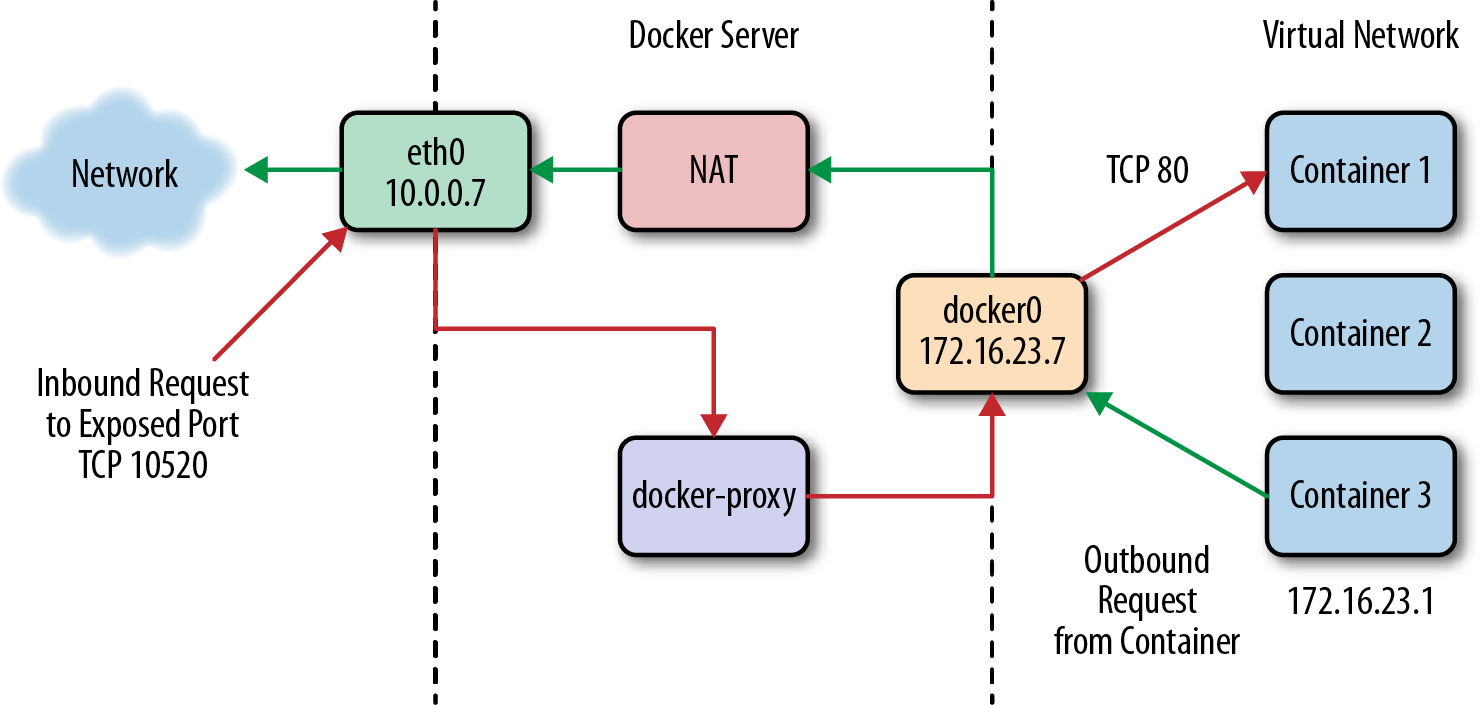
\includegraphics[width=.6\textwidth]{img/swarm-network}
\caption{Docker ma sieć \cite{docker_compose_reference}.}  \label{rys:network}% Źródło rysunku i etykieta przez którą odwołujemy się do rysunku.
\end{figure}

Jak widać na rys. \ref{rys:network} Docker ma wewnętrzną sieć. \lipsum[1]


\subsection{Rysunek z kotem}

Jak widać na rys.\ref{rysunek:kot} Ala ma kota. \lipsum[9-10] 

\begin{figure}[h!]
\centering
\includegraphics[width=.4\textwidth]{img/kotek}
\caption{Ala ma kota (opr.wł).}\label{rysunek:kot}
\end{figure}

\subsection{Tabela}

Co uwzględniono w tabeli \ref{tabela:coktoma}. \lipsum[13-15] 

% Tabela. Nazwa tabeli u góry.
\begin{table}[h!]
\centering\caption{Co kto ma \cite{harel_rzecz_2008} (patrz też dodatek~\ref{Dod1}) \label{tabela:coktoma}}
\begin{tabular}{|l|l|l|}% wyrównanie kolumn tabeli -> l c r - do lewej, środka, do prawej
\hline
Ala & ma & kota \\
\hline
Ola & ma & psa \\
\hline
Ula & ma & małpę\\
\hline
\end{tabular}
\end{table}

\lipsum[19-20] Warto wspomnieć, że w \cite{aizawa_groundwater_2009} rzecz przedstawiona jest zupełnie inaczej. Poniższy wzór:

\begin{equation}
\sum_{i=1}^{\infty}a_i
\label{eq:mojWzor}
\end{equation}

Wzór \ref{eq:mojWzor} wskazuje że dowód podany w \cite{kaleta_experimental_2005} może zostać podważony. \lipsum[9]

\section{Kod źródłowy}

% lub {java} albo {bash} albo {text}
\begin{listing}[h!]
\begin{minted}{c} 
int main()
{
   int a=2*3;
   printf("**Ala ma kota\n**");
   while(!I2C_CheckEvent(I2C1, I2C_EVENT_MASTER_MODE_SELECT)); /* EV5 */
   return 0;
}
\end{minted}
\caption{Przykładowy algorytm w języku C (opr. wł.)} \label{listing:moj}
\end{listing}

W moim kodzie \ref{listing:moj} zrobiłem coś wspaniałego. \lipsum[4]

\begin{table}[h]
	\begin{tabularx}{\textwidth}{|>{\setlength\hsize{1.4\hsize}\setlength\linewidth{\hsize}}X|>{\setlength\hsize{.9\hsize}\setlength\linewidth{\hsize}}X|>{\setlength\hsize{.7\hsize}\setlength\linewidth{\hsize}}X|}
		\hline
		\multicolumn{3}{|c|}{Classification of the criticel point $(0,0)$ of $x'=Ax,|\mathbf{A}|\not=0$.}\\
		\hline
		Types & Type of Critical Point & Stability \\
		\hline
		1. Real unequal eigenvalues of same sign
		\begin{itemize}
			\item $\lambda_1 > \lambda_2 > 0$
			\item $\lambda_1 < \lambda_2 < 0$
		\end{itemize} &
		\vphantom{1. Real unequal eigenvalues of same sign}
		\begin{itemize}
			\item Improper Node/Node
			\item Improper Node/Node
		\end{itemize} &
		\vphantom{1. Real unequal eigenvalues of same sign}
		\begin{itemize}
			\item Unstable
			\item Asym. Stable
		\end{itemize}\\
		\hline
		2. Real unequal eigenvalues of opposite sign
		\begin{itemize}
			\item $\lambda_2 < 0 >\lambda_1$
		\end{itemize} &
		\vphantom{2. Real unequal eigenvalues of opposite sign}
		\begin{itemize}
			\item Saddle Point
		\end{itemize} &
		\vphantom{2. Real unequal eigenvalues of opposite sign}
		\begin{itemize}
			\item Unstable
		\end{itemize}\\
		\hline
		3. Equal eigenvalues \newline Subtype 1: Two Independent vectors
		\begin{itemize}
			\item $\lambda_1 = \lambda_2 > 0$
			\item $\lambda_1 = \lambda_2 < 0$
		\end{itemize} &
		\vphantom{3. Equal eigenvalues} \vphantom{ Subtype 1: Two Independent vectors}
		\begin{itemize}
			\item Proper Node
			\item Proper Node
		\end{itemize} &
		\vphantom{3. Equal eigenvalues} \vphantom{ Subtype 1: Two Independent vectors}
		\begin{itemize}
			\item Unstable
			\item Asym. Stable
		\end{itemize}\\
		\hline
	\end{tabularx}
\end{table}
\thispagestyle{normal}

    % !TeX spellcheck = pl_PL
\chapter*{Zakończenie}\label{ch:ending}
\section{Podsumowanie pracy}\label{sec:summary}
\todo{W pracy udało mi się dużo zrobić. \lipsum[17]}

\section{Możliwości dalszego rozwoju}\label{sec:future-development}
\todo{Mnóstwo innych rzeczy da się poprawić i rozwinąć. \lipsum[23]}
\thispagestyle{normal}


    % W pracy pojawią się tylko prace naprawdę cytowane.
    % \nocite{*}
    \cleardoublepage
    \bibliography{literatura}
    \bibliographystyle{dyplom}

    \newpage
    \phantomsection
    \addcontentsline{toc}{chapter}{\listfigurename}
    \listoffigures

    \newpage
    \phantomsection
    \addcontentsline{toc}{chapter}{\listtablename}
    \listoftables

    \newpage
    \listof{listing}{Spis kodów źródłowych}

    % !TeX spellcheck = pl_PL
% \appendixpage
% \addappheadtotoc

\appendix
\begin{appendices}
    \chapter{JDL}\label{app:jdl}
%    \inputminted{text}{../../merged-jdl.jh}
%    \begin{listing}[h!]
%        \caption{merged-jdl.jh (opr. wł.)} \label{listing:merged-jdl}
%    \end{listing}
\end{appendices}
\thispagestyle{normal}


\end{document}
